% !TEX TS-program = xelatex
% !TEX encoding = UTF-8 Unicode

% META-NET Language Whitepaper, Norwegian Bokmål and Nynorsk

%\documentclass[]{../metanetpaper}

\usepackage{booktabs}
\usepackage{longtable}
\usepackage{tabulary}
\usepackage{tabularx}
\usepackage{rotating}
\usepackage{makecell}
\usepackage{multirow}
\usepackage{colortbl}
\usepackage{polyglossia}
\usepackage{multicol,framed,lipsum}
\setmainlanguage{norsk}
\setotherlanguages{english}

\RequireXeTeX %Force XeTeX check
%\newcommand{\gil}[1]{{\bf !!!#1}}
%\newcommand{\bokmaal}[1]{} % {#1} to activate bokmaal, {} to deactivate
%\newcommand{\nynorsk}[1]{#1} % {#1} to activate nynorsk, {} to deactivate

\begin{document}

\renewcommand*{\figureformat}{\sffamily\thefigure\autodot}

\selectlanguage{norsk}
\maketitle

\hyphenation{clarin CLARIN net-work gjes-dal infor-masjons-sam-funnet nyno-data infor-masjons-sam-funnet You-Tube språk-bar-riera-ne }

\cleardoublepage

% --------------------------------------------------------------------------

\bsection*{Forord --- Preface}

\null
\pagestyle{empty} 

\pagenumbering{Roman} 
\setcounter{page}{3}
\pagestyle{scrheadings}

\begin{Parallel}[c]{78mm}{78mm}

\ParallelLText{\selectlanguage{norsk}
Dette dokumentet er del av ein serie som skal fremje kunnskap om språkteknologiens status og potensiale. Målgruppa er journalistar, politikarar, språkbrukarar, lærarar og andre interesserte. Tilgangen til, og nytta av, språkteknologi i Europa varierer frå språk til språk. Difor vil òg naudsynte tiltak for å støtte forsking og utvikling av språkteknologi vere ulike for kvart språk. Kva for tiltak som er naudsynte, avheng av fleire faktorar, til dømes kompleksiteten i eit gjeve språk og mengda språkbrukarar.

Forskingsnettverket META-NET, eit \emph{Network of Excellence} finansiert av Europakommisjonen, presenterer i denne serien  (jf.~s.~\pageref{whitepaperseries}) analysen sin av eksisterande språkressursar og teknologiar for dei 23 offisielle EU-språka og andre nasjonale og regionale språk i Europa -- mellom dei norsk. Resultata av denne analysen tyder på at det er betydelege hol i forsking og utvikling for alle språka. Denne detaljerte ekspertanalysen av den noverande situasjonen i denne serien vil vonleg bidra til å maksimere effekten av ny forsking.

Per november 2011 består META-NET av 54 forskingsinstitusjonar i 33 land (jf.~s.~\pageref{metanetmembers}) som samarbeider med kommersielle aktørar (IT-føretak, utviklarar og brukarar), offentlege etatar, ikkje-statlege organisasjonar, representantar for språksamfunn og universitet. I samarbeid med desse samfunnsrepresentantane er målet å skape ein felles teknologivisjon og å utvikle ein strategisk forskingsagenda for eit fleirspråkleg Europa innan år 2020.}

\ParallelRText{\selectlanguage{english}
This white paper is part of a series that promotes knowledge about language technology and its potential. It addresses journalists, politicians, language communities, educators and others. 
The availability and use of language technology in Europe varies between languages. Consequently, the actions that are required to further support research and development of language technologies also differs. The required actions depend on many factors, such as the complexity of a given language and the size of its community.

META-NET, a Network of Excellence funded by the European Commission, has conducted an  analysis of current language resources and technologies in this white paper series (p.~\pageref{whitepaperseries}). The analysis focused on the 23 official European languages as well as other important national and regional languages in Europe. The results of this analysis suggest that there are tremendous deficits in technology support and significant research gaps for each language. The given detailed expert analysis and assessment of the current situation will help maximise the impact of additional research.

As of November 2011, META-NET consists of 54 research centres from 33
European countries (p.~\pageref{metanetmembers}). META-NET is working
with stakeholders from economy (Software companies, technology
providers and users), government agencies, research organisations, non-governmental organisations, language communities and European universities. Together with these communities, META-NET is creating a common technology vision and strategic research agenda for multilingual Europe 2020.}
\ParallelPar
\end{Parallel}

\makefundingnotice

% --------------------------------------------------------------------------

\cleardoublepage
\selectlanguage{norsk}

\bsection*{Innhald --- Contents}

\renewcommand\contentsname{}
\tableofcontents

\selectlanguage{norsk}

\addtocontents{toc}{\protect\thispagestyle{empty}\protect}
\addtocontents{toc}{{\Large\textsf{\centerline{NORSK I DEN DIGITALE TIDSALDEREN}}\par}}

% --------------------------------------------------------------------------

\cleardoublepage

\setcounter{page}{1}
\pagenumbering{arabic} 
\pagestyle{scrheadings}

\ssection[Samandrag]{Samandrag}

\begin{multicols}{2}

% New executive summary for Norwegian in Norwegian nynorsk
Informasjonsteknologi påverkar kvardagen vår. Vi brukar datamaskiner når vi skriv, redigerer, reknar ut, søkjer etter informasjon, og i aukande grad også når vi les, høyrer på musikk, kikkar på bilete og ser på film. Vi har med oss små datamaskiner i lomma og brukar desse til å ringe, skrive e-post, innhente informasjon og til å underhalde oss sjølve kvar vi enn er. Men på kva måte verkar denne utstrakte digitaliseringa av informasjon, kunnskap og dagleg kommunikasjon inn på språket vårt? Vil språket vårt endre seg eller til og med forsvinne? Kva er sjansane for at norsk språk vil bestå?        

Mange av dei 6000 språka som finst i verda i dag vil ikkje overleve i det globaliserte digitale informasjonssamfunnet. Ein reknar med at minst 2000 språk kjem til å forsvinne dei kommande tiåra.  Andre vil framleis spele ei rolle i privatsfæren og lokalsamfunnet, men ikkje i det breiare offentlege liv som næringsliv og akademia. Statusen til eit språk avheng ikkje berre av talet på brukarar eller kor mange bøker, filmar og TV-stasjonar som nyttar språket, men også av i kor stor grad språket gjer seg gjeldande i den digitale verkelegheita og blir brukt i programvareapplikasjonar. 

I denne samanhengen slit norsk framleis med veksesmerter. I byrjinga av det tjueførste hundreåret eksisterte norsk språkteknologi berre i svært liten skala. Det fanst eit relativt godt system for omsetjing frå bokmål og nynorsk, der var stavekontroll, og det fanst også eit lite dialogsystem som svarer på spørsmål, medan folk flest lo av den dårlege kvaliteten til dei første talegjenkjenningsprogramma. Eit ambisiøst industrielt initiativ til utvikling av språkteknologi på Voss mislykkast. Innan høgare utdanning fanst det program for språkteknologi og datalingvistikk, og det eksisterte forsking på desse felta, men det mangla språkressursar og språkverktøy.            

Biletet endra seg då Forskingsrådet tok initiativ til eit språkteknologiprogram i 2002, med sikte på å utvikle ny kunnskap og nødvendige verktøy. Programmet resulterte i fleire prosjekt som skapte ny kompetanse og eit betre grunnlag for norsk språkteknologi. Dei største prosjekta i dette språkteknologiprogrammet leverte eit tekst-til-tale-system og ein demonstrator for omsetjing av høg kvalitet frå norsk til engelsk.

Etter Stortingsmeldinga frå 2008 \cite{stm35:2008}, og vedtaket av
denne meldinga i Stortinget, vart ei fritt tilgjengeleg samling av
norske språkteknologiske ressursar, \emph{Språkbanken}, etablert i
2010. Språkbanken er no i gong med å byggje opp og distribuere norske
språkdata, ei oppgåve som lenge har vore etterspurd innan forsking og
utvikling. Dersom dette arbeidet blir halde ved like, vil det utgjere
ei uvurderleg investering i framtida til det norske språket.

Trass ei betydeleg utvikling innan norsk språkteknologi det siste tiåret viser denne rapporten at det enno berre er for basisverktøy og -ressursar at situasjonen er nokolunde tilfredsstillande. Når det gjeld meir avanserte applikasjonar, finst det framleis svært få verktøy og ressursar for norsk, og vi har framleis langt igjen før norsk språk er sikra ei framtid som fullverdig aktør i det moderne -- og framtidige -- europeiske språksamfunnet.   

Informasjons- og kommunikasjonsteknologien førebur seg no til neste teknologirevolusjon. I kjølvatnet av personlege datamaskiner, nettverk, stadig mindre og lettare komponentar, multimedia, mobile einingar og databehandling i digitale skyer, vil den neste generasjonen teknologi bestå av programvare som ikkje berre forstår talte og skrivne bokstavar og lydar, men også heile ord og setningar, og som støttar brukaren betre enn dagens teknologi, fordi han snakkar, kjenner og forstår språket deira. Forløparar i denne utviklinga er IBM si superdatamaskin Watson, som sigra over USA-meisteren i kunnskapsspelet “Jeopardy”, og Apple sin mobilassistent Siri for iPhone, som responderer på språkkommandoar og kan svare på spørsmål på engelsk, tysk, fransk og japansk. Eit norsk taleattkjenningssystem for iPhone er tilgjengeleg, men det er framleis mykje mindre påliteleg enn det tilsvarande engelske systemet. 

Språkbrukarar kommuniserer allereie ved hjelp av teknologien som er utvikla for deira språk. Etter kvart vil teknologiske innretningar, som respons på enkle talekommandoar, vere i stand til å hente dei viktigaste nyhenda og informasjonen frå den globale digitale kunnskapsbasen. Språkbasert teknologi vil kunne omsetje automatisk eller fungere som støtte for tolkar, lage samandrag av samtaler og dokument og vere eit hjelpemiddel i læringssituasjonar. Språkteknologi vil til dømes kunne hjelpe innvandrarar med å lære norsk, og dermed også med integrering i det norske samfunnet.        
 
Informasjons- og kommunikasjonsteknologi vil gjere industrielle
robotar og tenesterobotar (som i dag er under utvikling i
forskingslaboratoria) i stand til å forstå kva brukaren ønskjer at dei
skal gjere og til å rapportere om oppgåvene dei har utført. Eit slikt
prestasjonsnivå strekkjer seg langt ut over enkle bokstavlister og
leksika, stavekontrollar og uttalereglar. Skal språkteknologi kunne
tolke spørsmål og levere utfyllande og relevante svar, må han bevege
seg frå basale tilnærmingar til eit meir altomfattande perspektiv, der
språkmodelleringa tek omsyn til syntaks så vel som semantikk.  
\columnbreak

Ikkje alle europeiske språk er like godt førebudde til ei slik framtid. Denne rapporten presenterer ei evaluering av graden av språkteknologistøtte for 30 europeiske språk, basert på fire kjerneområde: maskinomsetjing, taleprosessering, tekstanalyse og, til sist, basisressursar som er naudsynte for å kunne byggje språkteknologiske applikasjonar. Språka vart delte inn i fem klynger etter nivå, og ikkje overraskande hamna norsk i botnklynga, og i enkelte tilfelle i klynga over, for alle typar verktøy og ressursar. Norsk ligg langt etter større språk som til dømes tysk og fransk. Men ikkje ein gong desse språka klarer å nå opp til kvaliteten og dekningsgraden til samanliknbare ressursar og verktøy for engelsk, som er det klart leiande språket på nesten alle felt innan språkteknologi.

I St.meld.~nr.~48 \cite{stm48:2002} konstaterer ein at språkteknologifeltet kan verte ``ein av dei fremste arenaene der kampen om norsk språk og kultur vil utspela seg i tida framover'' (kap.~12.9, s.~196). Kva må vi så gjere for å sikre norsk språk ei framtid i informasjonssamfunnet? I 2002 anslo ei ekspertgruppe skipa av myndigheitene at det vil krevje ei investering på 20 millionar kroner \emph{kvart år} dei første fem åra \cite{SR:2002:eng}. Sjølv om Språkbanken no er etablert og verksam, er det eit faktum at dei årlege investeringane så langt har utgjort berre ein brøkdel av estimert behov. Det skulle difor ikkje komme som noka overrasking at norsk språkteknologi framleis heng att i tidleg barndom. Kommersielt er fem millionar språkbrukarar for få til aleine å forsvare ei kostbar utvikling av nye produkt. Norsk IT-industri, og spesielt store og mellomstore bedrifter, kan ikkje sjølve ta kostnadene ved å byggje opp store språkressursar og verktøy for norsk. Framleis offentleg støtte er nødvendig for å sikre at eksisterande verktøy og opparbeidd kunnskap og erfaring hos forskarar og bedrifter skal bli utnytta til fulle. 

Norsk språk er ikkje umiddelbart trua av den engelske dominansen innan språkteknologi. Dette kan likevel endre seg drastisk når den nye generasjonen teknologiar tek til å meistre menneskeleg språk mykje betre, og meir effektivt, enn det dagens teknologi klarer. Gjennom utvikling innan maskinomsetjing vil språkteknologien på sikt medverke til å bryte ned språkbarrierar, men dette vil berre gjelde dei språka som er med på overgangen til eit digitalisert samfunn. Tilstrekkeleg og god nok språketeknologi kan sikre at språk med relativt små brukargrupper overlever. Som ein konsekvens er ei investering i språkteknologi ein essensiell del av språkpolitikken også i framtida.                                

META-NET sin visjon er å leggje til rette for språkteknologi av høg kvalitet for alle språk. Teknologien vil såleis støtte politisk og økonomisk fellesskap gjennom kulturelt mangfald. Den vil vidare bryte ned eksisterande barrierar og byggje bruer mellom europeiske språk. Dette inneber at alle interessentar -- i politikk, forsking, næringsliv og samfunn -- må foreine krefter for framtida. 

Denne språkrapporten utgjer ein viktig del av META-NET sin strategiske handlingsplan. Oppdatert informasjon, som til dømes den siste versjonen av META-NET sitt visjonsskriv \cite{Meta1} eller plan for forskingsstrategi (Strategic Research Agenda, SRA), er begge å finne på META-NET si nettside: http://www.meta-net.eu.
\end{multicols}

\clearpage

\ssection[Språka våre står i fare]{Språka våre står i fare: Ei utfordring for språkteknologien 
}

\begin{multicols}{2}

Vi er vitne til ein digital revolusjon som påverkar kommunikasjonen og samfunnet dramatisk. Den seinaste utviklinga i digital informasjons- og kommunikasjonsteknologi blir nokre gonger samanlikna med Gutenbergs oppfinning av trykkpressa. Kva kan denne analogien fortelje oss om framtida for det europeiske informasjonssamfunnet generelt og for stillinga til språka spesielt? 

\boxtext{Vi er vitne til ein digital revolusjon som kan samanliknast med Gutenbergs oppfinning av trykkpressa.}

I kjølvatnet av Gutenbergs oppfinning skjedde fleire store gjennombrot i kommunikasjon og kunnskapsutveksling, som til dømes Luthers omsetjing av Bibelen til eige morsmål. Sidan Gutenbergs tid har ein utvikla fleire teknikkar for betre handsaming av språkbehandling og kunnskapsutveksling: 

\begin{itemize}
\item standardisering av rettskriving og grammatikk for dei vanlegaste språka har gjeve ei hurtigare spreiing av nye vitskaplege og intellektuelle idear;
\item utviklinga av offisielle språk har gjort det lettare for innbyggjarane å kommunisere innanfor visse (som oftast politiske) grenser; 
\item undervising og omsetjing mellom språk har bidrege til utveksling på tvers av språk; 
\item  etablering av redaksjonelle og bibliografiske retningsliner har sikra kvaliteten og tilgangen på trykt materiale; 
\item etablering av ulike medium som aviser, radio, fjernsyn, bøker og andre medium har dekt ei rekkje kommunikasjonsbehov. 
\end{itemize}

Dei siste tjue åra har informasjonsteknologi bidrege til å automatisere og forenkle mange av desse prosessane: 

\begin{itemize}
\item publiserings- og teksthandsamingsprogram har erstatta skrivemaskin og dokumentproduksjon; 
\item Microsoft PowerPoint har erstatta overheadtransparentar; 
\item e-post gjer det mogleg å sende og ta mot dokument raskare enn med ei faksmaskin; 
\item Skype tilbyr billege telefonsamtaler via Internett og legg til rette for videokonferansar; 
\item ulike format for lagring av lydar og video gjer det enkelt å utveksle multimedie-innhald; 
\item søkemotorar gjer det enkelt å søkje i nettsider; 
\item nettbaserte tenester som Google Translate produserer raske, omtrentlege omsetjingar; 
\item sosiale medium som Facebook, Twitter og Google+ forenklar hurtig kommunikasjon, samarbeid og informasjonsdeling. 
\end{itemize}

Sjølv om slike verktøy og program er nyttige, er dei enno ikkje i stand til fullt ut å fylle rolla som ein berebjelke for innbyggjarane i eit fleirspråkleg europeisk samfunn, med fri flyt av informasjon og varer. 

\subsection[Språkgrenser hindrar utviklinga av eit europeisk informasjonssamfunn]{Språkgrenser hindrar utviklinga av eit europeisk informasjonssamfunn }

Vi kan ikkje føreseie nøyaktig korleis informasjonssamfunnet vil sjå ut i framtida. Men det er svært sannsynleg at den viktigaste revolusjonen i moderne kommunikasjonsteknologi vil liggje i nye måtar å samle folk som snakkar ulike språk. Dette legg press på den einskilde, som må lære nye språk, og på programutviklarar, som må lage nye applikasjonar som kan sikre gjensidig forståing og tilgjenge til deleleg kunnskap. I ein økonomi og eit informasjonssamfunn som blir stadig meir globalisert, vil nye medium føre til enklare interaksjon på tvers av språk, språkbrukarar og ulike typar innhald. Sosiale medium som Wikipedia, Facebook, Twitter, YouTube, og nyleg Google+ har vorte stadig meir utbreidde, men dette er berre toppen av isfjellet.

\boxtext{Ein stadig meir globalisert økonomi og informasjonssamfunn konfronterer oss med fleire språk, ulike språkbrukarar og ulike typar innhald.}

Ifølgje ein fersk rapport frå Europakommisjonen kjøper 57\% av Internettbrukarane i Europa varar og tenester på språk som ikkje er deira eige morsmål (engelsk er det vanlegaste framandspråket, følgd av fransk, tysk og spansk). 55\% av brukarane kan lese innhald på eit framandspråk, medan berre 35\% bruker eit anna språk til å skrive e-post eller poste kommentarar på nettet \cite{EC1}. For nokre år sidan var kanskje engelsk Internettet sitt \textit{lingua franca}, men no er situasjonen dramatisk forandra. Mengda av nettbasert innhald på andre europeiske språk (og dessutan asiatiske og språk frå Midtausten) har eksplodert. 

Denne digitale `klasseskilnaden' mellom språka har overraskande nok ikkje fått mykje offentleg merksemd, trass i at det gjennomsyrar heile samfunnet. Men det aktualiserer eit viktig spørsmål: Kva for europeiske språk vil overleve i eit nettverksbasert informasjons- og kunnskapssamfunn, og kva for språk er dømde til å forsvinne?

\subsection{Språka våre står i fare}

Medan trykkjeteknologien bidrog til å auke informasjonsspreiinga i Europa, førde han òg til språkdød. Regionale og minoritetsspråk vart sjeldan trykte, slik at språk som kornisk og dalmatisk vart avgrensa til munnleg overføring, noko som i sin tur avgrensa bruksområda. Vil Internett har same verknad på språka våre?

\boxtext{Det språklege mangfaldet i Europa er ein av dei viktigaste delane av kulturarven vår.}

Dei om lag 80 språka i Europa utgjer ein av dei viktigaste delane av kulturarven vår, og ein sentral del av den europeiske samfunnsmodellen \cite{EC2}. Medan språk som engelsk og spansk sannsynlegvis vil overleve på den nye digitale marknaden, risikerer mange europeiske språk å bli irrelevante i eit nettverksbasert samfunn. Dette ville kunne svekkje Europas posisjon på verdsbasis og svekkje målet om likeverdig deltaking for alle europeiske borgarar, uavhengig av språk. Ifølgje ein UNESCO-rapport om fleirspråklegheit er språk eit viktig middel for å nyte godt av grunnleggjande rettar, som politisk ytringsfridom, utdanning og samfunnsdeltaking  \cite{Unesco1}. 

\subsection{Språkteknologi kan leggje til rette for språkbruk}

Tidlegare vart det først og fremst investert i språkopplæring og omsetjing. Utrekningar viser at den europeiske marknaden for omsetjing, tolking, programvarelokalisering og nettstadsglobalisering utgjorde 8,4 milliardar euro i 2008, og dette talet blir forventa å vekse med 10\% årleg \cite{EC3}. Men denne investeringa dekkjer berre ein liten del av det noverande og framtidige behovet for kommunikasjon mellom språk. Eit viktig tiltak for å sikre breidda og mangfaldet av språkbruk i morgondagens Europa er å bruke riktig teknologi, akkurat som vi bruker teknologi til å løyse utfordringar innan transport, energi og universell utforming. 

Digital språkteknologi (retta mot alle former for tekst og munnleg tale) kan hjelpe menneske til å samarbeide, drive handel, dele kunnskap og delta i sosiale og politiske debattar på tvers av språkbarrierar og datakunnskapar. Språkteknologi er ofte innebygd i komplekse system som hjelper oss med å: 

\begin{itemize}
\item finne informasjon med ein Internett-søkemotor; 
\item sjekke staving og grammatikk i eit teksthandsamingsprogram; 
\item vise produkttilrådingane i nettbutikkar; 
\item høyre taleinstruksjonar frå eit bilnavigasjonssystem; 
\item omsetje nettsider via nettbaserte tenester. 
\end{itemize}

Språkteknologi består av ei rekkje kjerneapplikasjonar som legg til rette for ulike prosessar innanfor eit større applikasjonsrammeverk. Føremålet med META-NETs språkrapportar er å undersøkje i kva grad og kor godt desse kjerneteknologiane er utvikla for dei europeiske språka. 

\boxtext{Vi treng robust og rimeleg språkteknologi for alle dei europeiske språka.}

For å oppretthalde ein leiande posisjon i global innovasjon treng Europa ein språkteknologi som er tilpassa alle europeiske språk og som er robust, rimeleg og tett integrert i relevant programvare. Utan språkteknologi vil vi ikkje kunne skape ei effektiv, interaktiv, multimedial og fleirspråkleg brukaroppleving i den nære framtida.

\subsection{Språkteknologi gjev moglegheiter}

I ei verd basert på trykkjeteknologi var det viktige teknologiske gjennombrotet rask kopiering av ei tekstside ved hjelp av ei trykkpresse. Det omstendelege arbeidet med å slå opp, lese, omsetje og oppsummere kunnskap måtte framleis utførast av menneske. Ikkje før Edison kunne ein lagre tale, og då berre som analoge kopiar. 

Digital språkteknologi kan no automatisere sjølve omsetjingsprosessen, innhaldsproduksjon og kunnskapshandsaming for alle europeiske språk. Språkteknologi kan òg bidra til intuitive talestyrte grensesnitt for hushaldningsmaskiner, bilar, datamaskiner og robotar. Vi er enno på eit tidleg stadium av utviklinga av å bruke kommersielle og industrielle applikasjonar, men FoU har skapt mange nye høve. Til dømes er maskinomsetjing alt vorten rimeleg nøyaktig innanfor visse område, og eksperimentelle applikasjonar mogleggjer fleirspråkleg informasjons- og kunnskapsstyring og dessutan innhaldsproduksjon for mange europeiske språk. 

Som med dei fleste teknologiane vart den første bruken innan bl.a. talebaserte brukargrensesnitt og dialogsystem utvikla for svært spesialiserte domene, og dei hadde ofte ei nokså avgrensa yting. Men det ligg store marknadspotensial innanfor utdanningssektoren og underhaldningsindustrien ved å integrere språkteknologi i spel, kulturminnestader, skule og anna opplæring, bibliotek, osb. Mobile informasjonstenester, datastøtta språklæring, eLæringsmiljø, eigenvurderingsverktøy og plagiatkontrollprogram er berre nokre av bruksområda der språkteknologi kan spele ei viktig rolle. Populariteten til sosiale medium som Twitter og Facebook illustrerer behovet for avanserte språkteknologiar som kan overvake innlegg, oppsummere diskusjonar, analysere meiningstrendar, oppdage kjenslereaksjonar, identifisere brot på lover og reglar eller spore misbruk.

\boxtext{Språkteknologi kan bidra til å bryte\\ ned språkbarrierane som det\\ språklege mangfaldet skaper.}

Språkteknologi representerer eit enormt potensial for EU. Han kan
bidra til å handsame fleirspråklegheit i Europa – det faktumet at
ulike språk lever i naturleg sameksistens i europeiske føretak,
organisasjonar og skular. Men innbyggjarane treng å kommunisere på
tvers av desse språkgrensene og på kryss og tvers av den felles
europeiske marknaden. Språkteknologi kan bidra til å overvinne denne
siste barrieren samstundes som han støttar fri og open bruk av det
einskilde språket. Ser ein lenger framover, vil ein nyskapande og
fleirspråkleg europeisk språkteknologi gje ein målestokk for dei
globale partnarane våre når dei utviklar sine eigne fleirspråklege
samfunn. Språkteknologi er ei form for `hjelpemiddel'-teknologi som hjelper oss å bryte ned språklege barrierar og gjere språksamfunn meir tilgjengelege for kvarandre. 
Eit anna viktig og aktivt forskingsfelt er nytta av språkteknologi i redningsoperasjonar i katastrofeområde, der teknologiyting kan bli eit spørsmål om liv og død: Framtida sine intelligente robotar med tverrspråklege funksjonar kan redde liv. 
 
\subsection{Utfordringar for språkteknologi}

Sjølv om språkteknologien har gjort betydelege framsteg dei siste åra, skjer den noverande teknologiske utviklinga og produktinnovasjonen for sakte. Vanlege verktøy som stave- og grammatikkontroll i tekstbehandling er vanlegvis einspråklege og berre tilgjengelege for ei handfull språk. Nettbaserte maskinomsetjingstenester er nyttige for å få eit rask oversyn over innhaldet i dokumentet, men gjev store problem når svært nøyaktige og fullstendige omsetjingar trengst. På grunn av kompleksiteten i menneskeleg språk er det å modellere naturleg språkbruk i programvare for deretter å teste det ut i den verkelege verda ein tidkrevjande og kostbar operasjon som krev ei stabil finansiering. Dei europeiske landa må difor vere aktive i møte med dei teknologiske utfordringane eit fleirspråkleg samfunn står overfor gjennom aktivt å utvikle nye metodar for å skunde på utviklinga. Dette kan vere både utrekningsorienterte framsteg og teknikkar som `crowdsourcing'.

\boxtext{Den teknologiske utviklinga går for langsamt.}

\subsection{Språktileigning hos menneske og maskiner}

For å illustrere korleis datamaskiner handsamar naturleg språk, og kvifor det er vanskeleg å programmere dei til å prosessere ulike språk, skal vi kort sjå på korleis menneske tileignar seg første- og andrespråk, og deretter sjå korleis språkteknologiske system fungerer.

Menneske tileignar seg språkkunnskap på to ulike måtar. Babyar lærer eit språk ved å lytte til samspel mellom foreldre, sysken og andre familiemedlemmer. Frå toårsalderen produserer born dei første orda sine og korte setningar. Dette er berre mogleg fordi menneske har ein genetisk disposisjon til å imitere og rasjonalisere på grunnlag av det dei høyrer.

Å lære eit andrespråk på eit seinare stadium krev meir innsats, hovudsakleg fordi barnet ikkje er omgjeve av ein språkfellesskap, slik det er tilfelle for morsmålet. På skulen tileignar ein seg vanlegvis framandspråk gjennom å innarbeide grammatiske strukturar, ordtilfang og staving. Dette skjer ved hjelp av puggeøvingar som skildrar språklege kunnskapar gjennom abstrakte reglar, tabellar og døme.

\boxtext{Menneske tileignar seg språkkunnskap på to ulike måtar: Læring frå døme og læring frå underliggjande språkreglar.}

Dei to hovudtypane av språkteknologiske system `tileignar' seg språklege kunnskapar på ein liknande måte. Statistiske (eller `datadrivne') tilnærmingar innhentar språkkunnskap frå store samlingar av konkrete eksempeltekster. For å trene stavekontrollsystem er det tilstrekkeleg å bruke tekst frå eit enkelt språk, men skal ein trene opp eit maskinomsetjingssystem, treng ein eit sett av parallelle tekster for to (eller fleire) språk. På denne måten kan maskina `lære' mønster for korleis ord, korte setningar og fullstendige setningar blir omsette.

Ei statistisk tilnærming kan krevje millionar av setningar, og kvaliteten aukar jo meir tekst som blir analysert. Dette er ein av grunnane til at søkemotorleverandørar vil samle inn så mykje tekst som mogleg. Tekstbehandlingsprogramma sine stavekontrollar, så vel som tenester som Google Search og Google Translate, er alle baserte på statistiske metodar. Den store fordelen med statistiske metodar er at maskina lærer raskt gjennom ein kontinuerleg serie av treningsrundar, men kvaliteten er varierande.

Den andre tilnærminga til språkteknologi, og særleg til maskinomsetjing, er å byggje regelbaserte system. Språkforskarar, datalingvistar og dataekspertar må først kode grammatiske analysar (omsetjingsreglar) og setje saman ordlister (leksikon). Dette er svært tid- og arbeidskrevjande. Nokre av dei viktigaste regelbaserte maskinomsetjingssystema har vore under kontinuerleg utvikling i meir enn tjue år. Den store fordelen med regelbaserte system er at ekspertane har ein betre kontroll over maskina si språkhandsaming. Dimed kan ein systematisk rette opp feil i programvara og gje brukaren detaljerte tilbakemeldingar. Dette er spesielt nyttig når systema skal brukast til språklæring. Men på grunn av dei høge kostnadene har regelbasert språkteknologi så langt berre vorte utvikla for store språk.

\boxtext{Dei to hovudtypane av språkteknologiske system tileignar seg språk på ein liknande måte.}

Sidan styrkane og veikskapane ved statistiske og regelbaserte system ofte utfyller kvarandre, fokuserer forskinga no på hybridtilnærmingsmåtar som kombinerer dei. Så langt har likevel nytta av desse metodane vore mindre vellukka i industrielle applikasjonar enn i forskingslaboratoria. 

I dette kapitlet har vi sett at mange vanlege dataprogram er avhengige av språkteknologi. Dette gjeld særleg for Europa, i kraft av å vere eit felles økonomi- og informasjonsområde. Sjølv om kvaliteten på språkteknologi har vorte mykje betre dei siste åra, er det enno eit stort forbetringspotensial. Under vil vi skildre rolla 
norsk språk har i det europeiske informasjonssamfunnet og vurdere tilstanden for norsk språkteknologi. 
\end{multicols}

\clearpage

\ssection[Norsk i det europeiske informasjonssamfunnet]{Norsk i det europeiske informasjonssamfunnet}

\begin{multicols}{2}

\subsection{Generelle fakta}

Norsk er felles tale- og skriftspråk i Noreg, og er morsmålet til det store fleirtalet av den norske folkesetnaden (meir enn 90 \%, om lag 4.320.000 språkbrukarar). 
Norsk blir brukt i politikk og offentleg forvalting, på alle nivå i utdanningssystemet og i dagleg kommunikasjon.

\boxtext{Norsk er morsmålet til meir enn 90\%\\ av den norske folkesetnaden.}

Minoritetsspråka (slik dei blir definerte i Den europeiske pakta om regionale språk eller mindretalsspråk) i Noreg er samisk, kvensk, romanes og norsk romani. Kvar av desse gruppene omfattar frå nokre hundre til fleire tusen språkbrukarar \cite{stm35:2008}. 
Norsk teiknspråk blir brukt av om lag 15.000 språkbrukarar \cite{Erl:2007}. 
I tillegg finst det ulike innvandrarspråk. 
Innvandrarar og personar fødde i Noreg med innvandrarforeldre utgjer 600.900 personar eller 12,2\% av folkesetnaden i Noreg. Dei fleste av innvandrarane er frå Polen, Sverige, Tyskland og Irak, i følgje Statistisk sentralbyrå.

Norsk er eit nordgermansk språk som er nært nærskyldt med dansk og svensk, og desse tre språka er gjensidig forståelege. 
Norsk har eit stort mangfald av dialektar. 
Sjølv om såkalla `standard austnorsk' fungerer som ein \textit{de facto} standard for normalisert tale, er ei slik standardisering i langt mindre grad verksam i Noreg enn i dei fleste andre europeiske landa.
Norsk har to offisielle målformer, bokmål og nynorsk. Formelt har dei lik status, men i praksis er bokmål den desidert mest brukte, og blir brukt av om lag 87\% av innbyggjarane \cite{stm35:2008}. 
For å sikre stillinga til nynorsk regulerer \textit{Mållova} skriftleg språkbruk i offentleg sektor, og alle elevar lærer både bokmål og nynorsk på skulen, sjølv om der finst politiske rørsler som vil avskaffe dette kravet.

\subsection{Særtrekk ved norsk språk}

Norsk har ei rekkje særtrekk som bidreg til språkleg rikdom, men som samstundes skaper utfordringar for automatisk prosessering av naturleg språk.

\subsubsection{Utfordringar i norsk talespråk}
Munnleg norsk omfattar eit breitt utval av dialektar, som tradisjonelt har ei mykje meir framtredande rolle enn i dei fleste andre europeiske landa \cite{stm35:2008}.
Sidan ei munnleg standardnorm vanlegvis ikkje blir brukt i norsk, bruker språkbrukarane stort sett dialekten sin i munnleg kommunikasjon, også i media, om enn nokre gonger i moderert form. 
Dialektvariasjon er ei utfordring for datamaskiner når ein freistar å konvertere tale til tekst eller tekst til tale.

\boxtext{Noreg sitt dialektmangfald er ei utfordring\\ når ei datamaskin skal konvertere tale\\[.3mm] til tekst eller tekst til tale.}

Som i andre germanske språk kan ein på norsk danne nye ord ganske fritt ved å setje saman eksisterande ord. Til dømes kan orda \textit{oske}, \textit{krise} og \textit{pakke} setjast saman til \textit{oskekrisepakke}.
Nokre slike samansette uttrykk blir berre brukte av og til, medan andre utgjer terminologi i spesialiserte domene, og atter andre blir leksikaliserte (dvs. blir ein del av det vanlege ordtilfanget vårt) og inngår i ordbøker. 

Dessutan nyttar dei fleste norske dialektar tonefall kontrastivt gjennom to distinkte ordintonasjonar, ofte kalla tonem 1 og 2. Desse tonema, kombinert med eit manglande éin-til-éin-tilhøve mellom lydar og bokstavar i norsk, er særleg utfordrande for taleteknologi. Mellom anna har norsk eit breitt spekter av homografiske former (som blir likt skrivne) som blir realiserte med ulike tonem, til dømes  \textit{sulten} (tonem 1, eng.~`hunger') versus \textit{sulten} (tonem 2, eng.~`hungry'). Det er då avgjerande at eit talesyntesesystem kan oppgje rett tone til ein førekomst av eit leksem, i dette tilfellet ved å oppgje korrekt ordklasse, såkalla syntaktisk disambiguering. 

Ved konvertering frå tekst til tale er syntaktisk disambiguering naudsynt for å skilje mellom homografar som er ulike både når det gjeld tone og ordklasse, slik som para \textit{landa} {[}lanA{]} (tonem 1, eng.~`the countries') versus \textit{landa} {[}lanA{]} (tonem 2, eng.~`landed'). 
Faktisk har dei fleste inkjekjønnssubstantiv korresponderande homografiske verb. 

\subsubsection{Utfordringar i skriftleg norsk}

Når det gjeld skriftleg norsk, er der stor variasjon mellom dei to offisielle norske målformene både med omsyn til rettskriving og ordformasjon, og òg i nokre delar av ordtilfanget og grammatikken. 

I praksis er kravet om tospråklegheit i forvaltninga og utdanningssektoren nokre gonger vanskeleg å møte, sidan skilnadene kan opplevast som vanskelege å lære. Det blir gjort ein stor innsats for å oppretthalde denne tospråklegheita, og behovet for korrekturlesing og nøyaktig omsetjing mellom dei to formene er difor klart. Sjølv innanfor den enkelte målforma er stor variasjon tillaten i form og bøying av ord. Ordet \textit{slukke} kan til dømes òg skrivast som \textit{slokke} på bokmål (\textit{sløkke} eller \textit{sløkkje} på nynorsk), medan fortidsformene på bokmål kan vere \textit{slukket}, \textit{slukka}, \textit{slokket} eller \textit{slokka}. 

\boxtext{Endringar i rettskriving, ordtilfang og ordformasjon gjer at eksisterande språkressursar kan trenge ei oppdatering.}

Sjølv om ikkje alle moglege kombinasjonar av ord og endingar blir brukte i praksis, er kombinasjonsalternativa likevel formidable, og fører nokre gonger til tusenvis av moglege måtar å skrive same setning. 

For å komplisere saka endå meir har det norske skriftsystemet ikkje vore stabilt, fordi ei rekkje rettskrivingsreformer har vorte vedtekne opp gjennom åra, noko som tyder at eksisterande språkressursar kan ha bruk for ei oppdatering. 

Som nemnt i avsnittet om særtrekk ved norsk talespråk, er samansette ord på norsk ei utfordring for all språkteknologi fordi det krev gode analyseverktøy for slike uttrykk.
Ei av fleire utfordringar i omsetjing er bruk av norske refleksiv som i desse døma:

\smallskip
\emph{Per visste ikkje at Kari hadde freista å reparere bilen \emph{sin}.}

\smallskip
Ei korrekt omsetjing føreset ein djup grammatisk analyse av denne setninga. 

\subsection{Nyare utviklingstrekk}

I løpet av det siste tiåret har Språkrådet fatta ei rekkje vedtak som skal forenkle rettskriving i dei to målformene og gjere dei meir sameinte med den faktiske bruken. Ein har gått bort frå det tidlegare politiske målet om å slå dei to målformene saman, og variasjonen har i staden vorte redusert, sjølv om det enno er ein betydeleg grad av fridom. 

Utanlandske filmar og fjernsynsprogram er vanlegvis ikkje dubba til norsk (i motsetnad til i mange andre land, som Tyskland og Spania), noko som gjer at generasjonar av nordmenn har vore sterkt eksponerte for engelsk, særleg i oppveksten. 

Denne eksponeringa har truleg auka gjennom bruken av Internett. 
Difor har mange nordmenn gode ferdigheiter i engelsk. 
Nærveret av engelsk blir gjenspegla i lånord frå engelsk, men ei undersøking av nye ord i norske aviser i løpet av dei siste ti åra viser at berre rundt 5\% av nyorda kjem frå engelsk \cite{And:2011}.

\boxtext{Med eit domenetap for engelsk innanfor visse domene kan norsk bli delvis ubrukeleg som kommunikasjonsspråk.}

Likevel uttrykkjer språkpolitikarar ei bekymring \cite{nih:2005} for at norsk taper terreng innanfor visse domene, til dømes i IKT, næringsliv, økonomiske og administrative domene. 
Eit såkalla domenetap tyder at eit anna språk (engelsk, i tilfellet vårt) blir hovudspråket innanfor eit bestemt område, noko som tyder at nye norske termar ikkje lenger blir produserte i dette domenet. Dermed kan norsk bli delvis ubrukeleg som kommunikasjonsspråk, både mellom ekspertar på feltet og mellom ekspertar og ålmenta. 

Ironisk nok kan fråværet av tilfredsstillande norske termar bidra til at språkbrukarane utviklar ei generell haldning om at det er lettare å uttrykkje noko på engelsk. 

Sidan det generelt er vanskelegare å uttrykkje seg riktig og effektivt på eit framandspråk, er det viktig å auke medvitet om domenetap, fordi vi risikerer å ekskludere dei som ikkje kan engelsk frå å ta del i informasjonssamfunnet. 
Omsetjingar og forklaringar bør gjerast tilgjengelege der dette er naudsynt.

\subsection{Språkpolitikk i Noreg}

Media speler ei betydeleg rolle for bevaringa av språk, og i norske medium er statusen til det norske språket udiskutabel. Det er 13 radiokanalar og 19 TV-kanalar som sender over heile Noreg (regionale og lokale radiokanalar ikkje inkluderte), og alle sender primært på norsk, bortsett frå nokre program på samisk og på teiknspråk. 
Alle framandspråklege program er teksta på norsk, bortsett frå nokre barneprogram som vanlegvis er dubba og program på andre skandinaviske språk som ein reknar at blir forstått. 
Ved direktesendingar på andre språk, også på engelsk, omset eller oppsummerer som regel norsktalande kommentatorar høgdepunkta.

Norsk er ikkje etter lova definert som nasjonalspråk i Noreg, og det har vorte sagt ironisk at det finst lover for å verne minoritetsspråk og standardnynorsk, men ingen språkpolitikk for å verne norsk \cite{nih:2005}. 
Tre viktige lover styrer språkpolitikken. Den mest kjente er \textit{Mållova} av 1980, i tillegg har vi \textit{Samisk språklov} (1987) og \textit{Lov om stadnamn} (1990) \cite{stm35:2008}.

Kulturdepartementet har det overordna ansvaret for norsk språkpolitikk, medan Språkrådet er autorisert til å utvikle og setje i verk den gjevne politikken. Språkrådet i Noreg har eit meir omfattande ansvar enn tilsvarande instansar i Sverige og Danmark. 
Mellom anna har det ansvar for tilsyn og standardisering av språket, for styrking av norsk i samfunnet, for dei to målformene, og for å ta seg av norsk teiknspråk og minoritetsspråk. 
Språkrådet har spelt ei viktig rolle for å få behovet for norsk språkteknologi på den politiske dagsordenen. 
Gjennom rapportar til regjeringa, strategidokument og mediedekning har dei fremja synet om at språkteknologi er viktig for Noreg, både økonomisk og kulturelt.

\boxtext{Språkbanken, oppretta i 2010, skal vere ein infrastruktur for bevaring og deling av språkressursar og utviklingsverktøy for både forsking og industri}

Språkrådet bidrog også til å overtyde politikarane om at \textit{Språkteknologisk ressurssamling for norsk – Språkbanken} burde etablerast som eit språkpolitisk verkemiddel, og dette synet vart fremja i fleire rapportar som finst på \url{http://www.sprakradet.no/nb-NO/Tema/IKT--sprak/Norsk-sprakbank/}.
Språkbanken er meint som ``ei teneste til den delen av næringslivet som arbeider med utvikling av språkbasert IKT, til forskarar innan språkvitskap og språkteknologi, og til offentlege verksemder som utviklar elektroniske løysingar for offentlege tenester.'' %\footnote{http://www.nb.no/spraakbanken/}. 
Meir konkret skal Språkbanken vere ein infrastruktur for bevaring og deling av språkressursar og utviklingsverktøy for både forsking og industri. 
I etterkant av stortingsmeldinga \textit{Mål og meining} \cite{stm35:2008} fekk Nasjonalbiblioteket i oppdrag å etablere Språkbanken og å starte innsamling og utvikling av språkressursar som skulle innlemast. 
Sidan juni 2011 er fleire språkressursar lagt ut, og er no fritt tilgjengeleg for nedlasting, gjennom Språkbanken, og nye ressursar er under utvikling.
Oppdatert informasjon finst på \url{http://www.nb.no/spraakbanken/}.

Stortingsmeldinga \textit{Mål og meining} understreka òg at terminologiske ressursar i Noreg har betydelege manglar med omsyn til dekningsgrad og at der difor er eit behov for oppdatering. Eksisterande terminologiressursar varierer sterkt med omsyn til format, innhald, struktur og metadata. 
Sidan bevaring av norsk terminologi er eit viktig språkpolitisk spørsmål, gav Språkrådet i Noreg, med økonomisk støtte frå Kulturdepartementet, selskapet Standard Noreg i oppdrag å utvikle ein fritt tilgjengeleg termbase med terminologi på fleire språk \cite{drosdal2010}. 
Denne termbasen vart gjord offentleg tilgjengeleg for nettsøk i 2011, men er så langt ikkje vorten gjord tilgjengeleg for nedlasting og bruk i vidare FoU. 
 
\subsection{Språk og utdanning}

Nyare forsking tyder på at ein ikkje bør undervurdere kor viktig språk er i utdanningssamanheng. 
Frå eit språkteknologisk synspunkt er behovet for gode skriftlege hjelpemiddel difor klart. 

Den første PISA-undersøkinga (2000) viste at norske elevar skåra marginalt over OECD-gjennomsnittet med omsyn til leseferdigheiter. 
Debatten i etterkant auka det offentlege medvitet om språklæring, og fleire nasjonale tiltak vart difor sette i verk for å stimulere norske elevar sine leseferdigheiter. 

I den siste PISA-testen i 2009  \cite{pisa2009eng} gjorde norske elevar det betydeleg betre med omsyn til leseferdigheiter (sjølv om gjennomsnittet i OECD òg har falle sidan 2000, noko som svekkjer verknaden av den tilsynelatande forbetringa hos norske elevar). 
Som i dei tidlegare PISA-testane var resultatet i 2009 særleg lågt for elevar med migrasjonsbakgrunn. 

\boxtext{Der er eit klart behov for gode språkteknologiske skrivestøtteverktøy innan utdanningssektoren.}

Når det gjeld leseferdigheiter hos vaksne, viser resultat frå undersøkinga ``Adult Literacy and Life Skill'' (ALL) at leseferdigheita hos 300.000 vaksne nordmenn, eller ein av ti, er så låg at dei får problem i det moderne samfunnet  \cite{gab:2005}. 
I undersøkinga blir individa sine leseevner rangerte på ein skala frå 1 til 5 for ulike område. Ifølgje OECDs definisjon vil lesarar på nivå 1 og 2 innanfor minst eitt av områda få problem i eit moderne informasjonssamfunn. I Noreg gjeld dette om lag 1 million lesarar. 

Behovet for å lære både bokmål og nynorsk er eit kontroversielt tema i Noreg. I skulen avgjer kommunen hovudmålet i grunnskulane frå og med første klassa, medan sidemålsundervisinga vanlegvis blir introdusert i sjuande klassa. I dag har om lag 87\% av alle norske elevar nynorsk som sidemål \cite{SR:2010}. %(p. 42). 
I hovudsak har dei med nynorsk som hovudmål få problem med å lære å meistre bokmål sidan dei er eksponerte for bokmål gjennom media og litteratur frå barnsbein av. Fleirtalet av elevane, som altså har bokmål som hovudmål, opplever derimot ofte problem med å meistre nynorsk sidan dei har fått mindre opplæring og vore mindre eksponerte for det. 

Statusen til norsk som skulefag i grunnskulen gjenspeglar til ei viss grad behovet for å prioritere leseferdigheiter. Ei undersøking publisert av Utdanningsdirektoratet i 2009 viser at norskfaget utgjer om lag 26\% av undervisningstida for elevar mellom 6-12 år. 
På dette området ligg det norske skulesystemet nær Frankrike, Hellas og Nederland, der nesten ein tredjedel av undervisningstida for 9-til-11-åringar er i morsmålsopplæring.

Eit anna aspekt ved rolla til språket i opplæringa er at norskopplæring har vorte ein del av utlendingspolitikken i Noreg. 
I 2003 vart den såkalla \textit{Introduksjonslova} vedteken. I følgje denne lova har innvandrarar rett og plikt til 300 timar undervising i norsk språk, historie, kultur og lovgjeving. 
I følgje \textit{Utlendingslova} av 2008 er oppfylling av denne plikta ein av føresetnadene for å kunne få permanent opphald i Noreg. 

Eit aktuelt tiltak for å gje elevar naudsynte språkferdigheiter for aktiv deltaking i samfunnet er å auke mengda av norskundervising i skulen. 
Språkteknologi kan vere eit viktig bidrag gjennom såkalla dataassistert språklæring (\textit{computer-assisted language learning}; CALL), system som lèt elevane oppleve språk på ein attraktiv måte, til dømes ved å knyte vokabular i elektroniske tekster til lett forståelege definisjonar eller til lydar- eller videofiler som kan gje tilleggsinformasjon om til dømes uttale. 

\subsection{Inkluderingsaspekt} 

Det er eit uttalt politisk mål i Noreg å sikre alle innbyggjarar like vilkår for deltaking. 
Fleire lover gjeld spørsmålet om inkludering, til dømes i \textit{Diskriminerings- og tilgjengelegheitslova} og \textit{Lov om opplæring}, som spesifiserer at utdanning skal tilpassast behovet til den einskilde. Særlig viktig er \textit{Diskriminerings- og tilgjengelegheitslova}, som spesifiserer at nye IKT-løysingar retta mot ålmenta, til dømes sosiale nettverk eller offentlege nettsider, skal tilfredsstille lovkrava om tilgjenge innan 1. juli 2011. 
Innan 2025 skal alle IT-løysingar tilfredsstille lovkrava. 

\boxtext{Innan 2025 skal alle IKT-løysingar retta mot ålmenta, til dømes sosiale nettverk eller offentlege nettsider, tilfredsstille lovkrava om tilgjenge.} 

Tekstbaserte kommunikasjonsmedium (SMS, e-post, Facebook, blogging, Twitter) har i løpet av svært kort tid endra måten vi kommuniserer på. 
Mykje fagleg og personleg kommunikasjon, og til og med viktige offentlege debattar, føregår på Internett. Slike digitale nettverk krev at tekster av høg kvalitet blir produserte raskt. 

For dei fleste er nett- og tekstbasert kommunikasjon ein rikdom, men ikkje alle er komfortabel med denne kommunikasjonsmåten. 
For det første har anslagsvis 5\% av innbyggjarane alvorleg dysleksi, medan så mange som 20\% av dei mellom 16 og 20 år har generelle lese- og skrivevanskar, ifølgje Dysleksiforbundet. 
For det andre er mange språkbrukarar med norsk som andrespråk framleis i ein læringsprosess. 
Omtrent to av tre innvandrarar har svake leseevner \cite{gabrielsen2007}.
For det tredje skriv grupper av rørslehemma, svaksynte eller blinde brukarar ofte feil fordi dei mistolkar talerespons eller er ikkje registrerer feil som akkurat er gjort. 
Alle desse gruppene kan oppleve større problem med tekstbruk under tidspress. 
Personar med motoriske vanskar kan òg oppleve problem med tekstbruk og treng ofte spesielt tilpassa løysingar.

Med andre ord er det ein reell fare for at desse gruppene vil bli hindra frå å dra full nytte av slike tekstbaserte kommunikasjonsmedium, med mindre dei får tilgjenge til brukarvennlege verktøy som kan støtte kommunikasjonsprosessen. 
Til sjuande og sist er denne utfordringa potensielt eit demokratisk problem. 
Brukarvennlege språkteknologiske verktøy er her eit av dei viktigaste grepa for å oppfylle lova om universell utforming og å syte for at alle blir inkluderte.

\subsection{Internasjonale aspekt}

Engelsk er utan tvil det dominerande språket i norske vitskaplege publikasjonar. Ein studie frå 2004 viste at om lag åtte av ti vitskaplege artiklar skrivne av norske forskarar vart utgjevne på engelsk; meir enn ein tredjedel av desse vart publiserte utanfor Noreg \cite{schwach2004}.

Vi ser den same engelske dominansen i næringslivet \cite{SR:2010,Hel:2010}. 
Ein stadig meir internasjonal arbeidsstokk skaper fleirspråklege arbeidsplassar der engelsk blir arbeidsspråket. 
Noreg har ein eksportbasert økonomi, og er tungt involvert i internasjonal humanitær, diplomatisk og militær aktivitet; sistnemnde i regi av SN eller NATO. 
Gode kunnskapar i engelsk og andre framandspråk er difor viktig for nordmenn på mange område, frå næringsliv og høgare utdanning til det militære, politikk og diplomati. 
Engelsk er det mest brukte framandspråket, og sjølv om nordmenn har ord på seg for å vere dugelege i engelsk, manglar likevel mange språkbrukarar dugleiken som trengst for avansert bruk i jobbsamanheng. 
Ei rekkje av dei spurde i departementa meiner at bruk av engelsk går utover Noregs innverknad til dømes i forhandlingar på europeisk nivå, medan bruken av engelsk i næringslivet har ført til veikte forretningsmogelegheiter og til og med tap av kontraktar.

\boxtext{Fungerande system for maskinomsetjing vil vere avgjerande for å gje nordmenn fridomen til å bruke morsmålet sitt i framtida. }

Språkteknologi kan møte denne utfordringa frå eit anna perspektiv ved å tilby tenester som maskinomsetjing eller tverrspråkleg informasjonsinnhenting, og dermed bidra til å redusere dei personlege og økonomiske ulempene som dei som ikkje har engelsk som morsmål ofte møter. 
Faktisk vil maskinomsetjing vere avgjerande for å gje nordmenn fridomen til å halde fram å bruke morsmålet sitt i framtida. 
I situasjonar der nordmenn treng å kommunisere på engelsk, står ein som regel overfor valet mellom å skrive dokument éin gong på engelsk, eller dobbelt opp på engelsk og norsk. 
Med eit fungerande norsk-til-engelsk maskinomsetjingssystem kan norsk oppretthaldast som arbeidsspråk i Noreg.

\subsection{Norsk på Internett}

I 2010 hadde om lag 93\% av norske innbyggjarar internettilgang ifølge MedieNorge. 
Omtrent 68\% var på nettet kvar dag; blant unge er talet endå høgare. 
Ein studie frå 2010 viste at meir enn 2,5 millionar nordmenn, om lag halvparten av innbyggjarane, har ein Facebookprofil, noko som plasserer nordmenn blant dei mest dedikerte brukarane av dette sosiale mediet. 
Estimat viser at det finst om lag 34 millionar nettsider på norsk. 

\boxtext{Den aukande bruken av Internett speler ei viktig rolle for språkteknologi.} 

Den enorme mengda digitale språkdata er ein viktig ressurs for å analysere nytta av naturleg språk, spesielt for innsamling av statistisk informasjon om språkmønster. Internett omfattar òg eit breitt utval av bruksområde for språkteknologi. 

I Noreg er ein i ferd med å utvikle to forskingsdrivne tekstkorpus basert på tekst frå Internett. 
Det største tilgjengelege norske korpuset per i dag er Norsk aviskorpus, eit monitorkorpus av norske avistekster publiserte på nett. 
Korpuset er utvikla i samarbeid mellom NHH i Bergen og Uni Research, Bergen. Korpuset er no på over 900 millionar ord og blir utvida i gjennomsnitt med 1 millionar ord i veka, dvs. ei mengd ord tilsvarande om lag 10 romanar. 
Det andre internettkorpuset, NoWaC, er utvikla ved Tekstlaboratoriet ved Universitetet i Oslo, og inneheld om lag 700 millionar ord lasta ned frå hovuddomenet .no. 

Når det gjeld parallell eller omsett tekst på Internett, er tilgjenget avgrensa for norsk samanlikna med andre europeiske språk. 
Omsette tekster til og frå norsk er vanskelege å finne (med unntak av tekster med relevans for EØS er EU-tekster generelt ikkje omsette til norsk), og slike ressursar er naudsynte for maskinomsetjing og programvare for omsetjingsminne. 
Sett i ljos av det forventa behovet har forholdsvis lite språkteknologi vorte utvikla og nytta for omsetjing av nettstader. 
Den mest brukte nettapplikasjonen er nettsøk, som inneber automatisk prosessering av språk på fleire nivå (dette vil bli gått gjennom i meir detalj seinare). Nettsøk føreset avansert språkteknologi som er ulikt for kvart språk. 
På grunn av dei to målformene i norsk, og dessutan betydelege variasjonar innanfor dei, må ein ofte gå gjennom ei omfattande mengd variantar av søkeord eller setningar som skal passe saman. 
Det neste kapitlet gjev ei innføring i språkteknologi og dei viktigaste bruksområda, saman med ei evaluering av dagens språkteknologi for norsk.

\end{multicols}

\clearpage

\ssection[Språkteknologisk støtte for norsk språk]{Språkteknologisk støtte for norsk språk}

\begin{multicols}{2}

Språkteknologiske verktøy og ressursar er programvare utvikla for å handsame menneskeleg språk, og blir difor ofte kalla `menneskeleg språkteknologi'. 
Menneskeleg språk finst i munnleg og skriftleg form. Medan tale er den eldste og evolusjonsmessig mest opphavlege forma for språkleg kommunikasjon, blir kompleks informasjon og det meste av menneskeleg kunnskap lagra og overført i skriftlege tekster. Teknologi for tale og tekst prosesserer eller produserer språk i høvesvis munnleg og skriftleg form, men begge typar teknologi brukar ordbøker og grammatiske og semantiske reglar. Dette tyder at språkteknologi knyter språk til ulike former for kunnskap, uavhengig av mediet (tale eller tekst) kunnskapen er uttrykt i. Figur~\ref{fig:ltincontext_no} illustrerer det språkteknologiske landskapet.

\begin{figure*}[htb]
  \colorrule{grey3}{\textwidth}{1.5pt}
  \center
  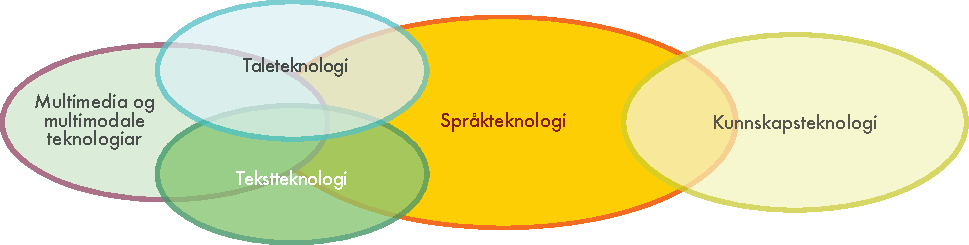
\includegraphics[width=\textwidth]{../_media/norwegian-nynorsk/language_technologies}
  \caption{Språkteknologi}
  \label{fig:ltincontext_no}
  \colorrule{grey3}{\textwidth}{1.5pt}
\end{figure*}

Når vi kommuniserer, kombinerer vi språk med andre kommunikasjonsmåtar
og informasjonsmedium – til dømes kan det å snakke omfatte både gestar
og andletsuttrykk. Digitale tekster kan knyte seg opp mot både bilete
og lydar. Filmar kan innehalde språk i både munnleg og skriftleg
form. Med andre ord er tale- og tekstteknologi overlappande, og dei
samhandlar med andre teknologiske verktøy som bidreg til handsaming av
multimodal kommunikasjon og multimediedokument.

I det følgjande vil vi diskutere dei viktigaste bruksområda for språkteknologi, dvs. korrekturlesing, nettsøk, taleteknologi og maskinomsetjing. 

Dette omfattar program og grunnleggjande teknologiar som:

\begin{itemize}
\item korrekturlesing
\item skrivestøtte
\item dataassistert språklæring
\item informasjonsinnhenting  
\item informasjonsekstrahering
\item tekstsamandrag
\item svar på spørsmål/dialogsystem
\item taleattkjenning 
\item talesyntese 
\end{itemize}

Språkteknologi er eit etablert forskingsfelt, og det finst eit omfattande utval av introduksjonslitteratur.

For vidare lesing tilrår vi lærebøkene \cite{jurafsky-martin01, manning-schuetze1}, oversiktsverka \cite{lt-survey1} og nettsida LT World (\url{http://www.lt-world.org}).

Før vi går vidare til ein diskusjon av desse bruksområda, skal vi kort skildre oppbygginga av eit typisk språkteknologisk system. 

\subsection[Applikasjonsarkitekturar]{Applikasjons- arkitekturar}

Dataprogram for språkhandsaming består typisk av fleire komponentar som gjenspeglar ulike aspekt ved språket. Slike applikasjonar er som oftast svært komplekse, og figur~\ref{fig:textprocessingarch_no} viser ein svært forenkla arkitektur for eit vanleg teksthandsamingsprogram. Dei tre første modulane handsamar strukturen og tydinga til den analyserte teksten:

\begin{enumerate}
\item Preprosessering: Reinsar data, analyserer eller fjernar formatering, identifiserer inndataspråk, osb. 
\item Grammatisk analyse: Finn verbet, identifiserer objekta til verbet, modifikatorar og andre setningskomponentar, identifiserer setningsstruktur. 
\item Semantisk analyse: Utfører disambiguering (dvs. bereknar tydinga av eit ord i ein gjeven kontekst); løyser opp anaforar (dvs. finn kva for pronomen som refererer til kva for substantiv i setninga); representerer setningstydinga på ein maskinleseleg måte.
\end{enumerate}

Etter tekstanalysen kan modular innretta mot spesifikke oppgåver takast i bruk, til dømes automatisk samandrag og databasesøk. 

I resten av denne kapitlet skal vi først gje ei skildring av dei viktigaste bruksområda for språkteknologi. Deretter følgjer eit kort oversyn over situasjonen for språkteknologisk forsking og utdanning i dag, saman med ei skildring av tidlegare og noverande forskingsprogram. Til slutt skal vi presentere eit ekspertestimat for dei viktigaste språkteknologiske verktøya og ressursane for norsk, vurdert etter ulike kriterium som tilgjenge, mogenskap og kvalitet. Den generelle situasjonen for språkteknologi for norsk språk er oppsummert i ein eigen tabell (figur~\ref{fig:lrlttable_no}), som gjev eit oppdatert oversyn over språkteknologi for norsk. Den språkteknologiske støtta for norsk språk er òg samanlikna med dei andre språka som er analyserte i denne kvitbokserien. 

\begin{figure*}[htb]
  \colorrule{grey3}{\textwidth}{1.5pt}
  \center
  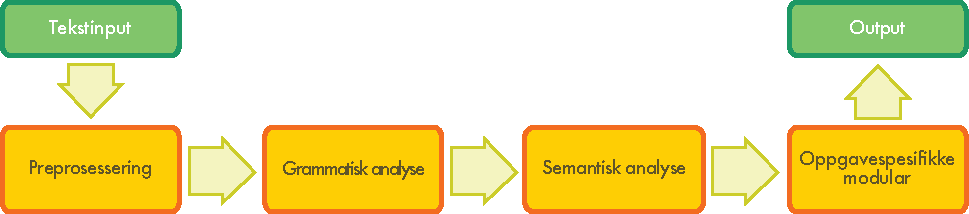
\includegraphics[width=\textwidth]{../_media/norwegian-nynorsk/text_processing_app_architecture}
  \caption{Ein typisk applikasjonsarkitektur for tekstprosessering}
  \label{fig:textprocessingarch_no}
  \colorrule{grey3}{\textwidth}{1.5pt}
\end{figure*}

\subsection{Dei viktigaste bruksområda}

I dette avsnittet fokuserer vi på dei viktigaste språkteknologiske verktøya og ressursane, og gjev eit oversyn over språkteknologisk verksemd i Noreg.  %GIL Verktøy og ressursar som er understreka i teksten, kan også finnast i tabellen på slutten av dette kapitlet.

\subsubsection{Korrekturlesing}

Alle som har brukt eit teksthandsamingsprogram som Microsoft Word veit at det har ein stavekontroll som uthevar stavefeil og føreslår rettingar. Dei første stavekontrollane samanlikna ei liste av utvalde ord mot ei ordbok med korrekte ord. I dag er slike program langt meir sofistikerte. Ved å bruke språkspesifikke algoritmar for \textbf{grammatisk analyse} kan dei oppdage morfologiske feil (t.d. fleirtalsformer) og dessutan syntaktiske feil, til dømes manglande verb eller gal verbbøying (t.d \textit{ho *skrive eit brev}). Men dei fleste stavekontrollar vil ikkje finne nokon feil i denne engelske teksten, fordi alle orda er korrekt stava, sjølv om enkelte av ordvala er feil \cite{zar1}:
 
\begin{quote}
  I have a spelling checker,\\
  It came with my PC.\\
  It plane lee marks four my revue\\
  Miss steaks aye can knot sea.
\end{quote}

For å avdekke slike feil trengst ei analyse av konteksten, til dømes for å avgjere om eit norsk ord skal stavast med enkel eller dobbel konsonant i norsk, som i \textit{vil} vs. \textit{vill}.
Denne typen analyse må anten baserast på språkspesifikke \textbf{grammatikkar} som ekspertar gjennom mykje arbeid har koda i programvara, eller på ein statistisk språkmodell. 
I ein statistisk modell reknar ein ut sannsynet for at eit bestemt ord finst i ein viss posisjon i teksten. Til dømes er \textit{eg vil ha} ein mykje meir sannsynleg ordsekvens enn \textit{eg vill ha}. Ein statistisk språkmodell kan genererast automatisk ved hjelp av ei stor mengd av (riktige) språkdata, eit \textbf{tekstkorpus}. 

Desse to tilnærmingane har i hovudsak vorte utvikla med utgangspunkt i materiale frå engelsk. Likevel kan ingen av dei enkelt overførast til norsk, sidan norsk har annleis ordstilling, samansette ord og eit meir omfattande bøyingsmønster for visse ordklasser enn engelsk. Studiar med utgangspunkt i norsk er difor naudsynt. Sidan norsk har to offisielle målformer, der den eine er mindre brukt, er behovet for gode korrekturverktøy for kvar av målformene stort. 

\begin{figure*}[htb]
  \colorrule{grey3}{\textwidth}{1.5pt}
  \center
  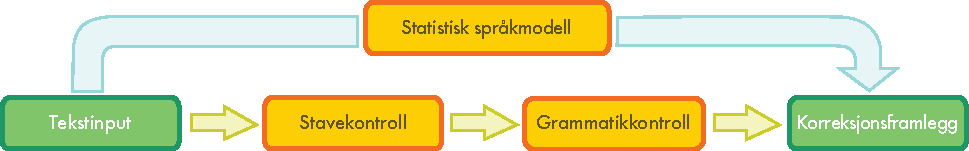
\includegraphics[width=\textwidth]{../_media/norwegian-nynorsk/language_checking}
  \caption{Korrekturlesing (over: statistisk; under: regelbasert)}
  \label{fig:langcheckingaarch_no}
  \colorrule{grey3}{\textwidth}{1.5pt}
\end{figure*}

Korrekturlesingsverktøy er ikkje avgrensa til teksthandsamingsprogram, det er òg brukt i “skrivestøttesystem”, dvs. programvaresystem som blir brukte for å skrive manualar og andre typar teknisk dokumentasjon som må oppfylle spesielle standardar til dømes innan IT- og helsesektoren og innan ingeniørverksemd. I frykt for kundeklager og skadekrav som følgje av uklare instruksjonar, fokuserer næringslivet i aukande grad på teknisk dokumentasjonskvalitet, samstundes som dei rettar seg mot ein internasjonal marknad (via omsetjings- eller lokaliseringstenester). Framsteg innan prosessering av naturleg språk har ført til utvikling av programvare for skrivestøtte. Slik programvare hjelper forfattarar av teknisk dokumentasjon til å bruke ordtilfang og setningsstrukturar som er i samsvar med industrireglar og (bedriftsinterne) terminologiske restriksjonar. 

\boxtext{Korrekturlesingsverktøy blir ikkje berre brukt til teksthandsaming, det blir også brukt i skrivestøttesystem.}

Gode korrekturlesingsverktøy kan vere ein viktig reiskap for personar med skrivevanskar, anten det er dyslektikarar eller andrespråkselevar, sidan ein kontekstsensitiv analyse gjer det mogleg å føreslå færre og meir relevante stavemåtar; det motsette, mange val, krev nettopp eit høgt nivå av leseferdigheit og språkleg medvit.

Nokre få norske selskap og språktenesteleverandørar utviklar produkt på dette området. 
I forskingssektoren blir det utvikla grunnleggjande språkteknologiske ressursar som kan vere av nytte for grammatikk- og stavekontroll (leksikon, ordlister, tekstkorpus, analyseverktøy for samansette ord); desse er i hovudsak utvikla ved Universitetet i Oslo, Universitetet i Bergen og Uni Research i Bergen. 

Det mest brukte korrekturverktøyet for norsk finst i Microsoft Office-pakka, og er laga av det finske firmaet Lingsoft, medan delar av grammatikkontrollen for bokmål vart utvikla av forskarar ved Universitetet i Oslo. Stavekontroll for bokmål og nynorsk med open kjelde-teknologi, som \textit{Hunspell}, er også tilgjengeleg. 

Ein annan norsk kommersiell aktør er Tansa, som spesialiserer seg på korrekturverktøy tilpassa dei spesifikke behova og ordtilfanget større føretak har. 
Dei dekkjer fleire språk i tillegg til norsk bokmål og nynorsk (til dømes engelsk, tysk, spansk og fransk), og kundane spenner frå NRK til Financial Times. 
Nynodata AS tilbyr eit omsetjingsverktøy frå bokmål til nynorsk som samstundes hjelper brukaren å følgje ein konsekvent formbruk. 

Tre selskap rettar seg spesifikt mot skriftlege hjelpemiddel for dyslektikarar. To av dei, Lingit og Include, inneheld ein stavekontrollmodul i tillegg til andre lese- og skriveverktøy (ordprediksjon, tekst-til-tale-komponentar), medan MikroVerkstedet tilbyr fullføring av ord og ordprediksjon. 

Ved første augnekast synest dermed situasjonen for korrekturverktøy på norsk å vere god. 
Men samstundes er fleire av initiativa nokså sårbare. 
Til dømes er norsk korrekturlesing basert på open kjeldekode (\textit{aspell, Hunspell}) driven av tre einskildpersonar som gjer dette på fritida. 
Med andre ord er ein av dei viktigaste norske konkurrentane til Microsofts programvare avhengig av eit personleg initiativ frå ei handfull idealistiske einskildpersonar, snarare enn ein systematisk innsats for å utvikle modular med open kjeldekode. 
Vidare er det ei viktig utfordring for dei fleste norske korrekturlesingsverktøya å \textit{forbetre} eksisterande ressursar ved å utvikle meir avanserte språkteknologiske verktøy. Det manglar òg språkspesifikke verktøy for automatisk omsetjing og omsetjingsstøtte. Verktøy med omsetjingsminne som Trados finst, men dei har inga språkspesifikk tilpassing til norsk utover ein grunnleggjande stavekontroll. 

Utover korrekturlesnad og skrivestøtte er korrekturverktøy òg viktig innanfor dataassistert språklæring. Korrekturverktøy kan òg automatisk korrigere nettsøk, som i Google sine \textit{Meinte du…}  -- forslag til korrekte nettsøk.

\subsubsection{Nettsøk}

\begin{figure*}[htb]
  \colorrule{grey3}{\textwidth}{1.5pt}
  \center
  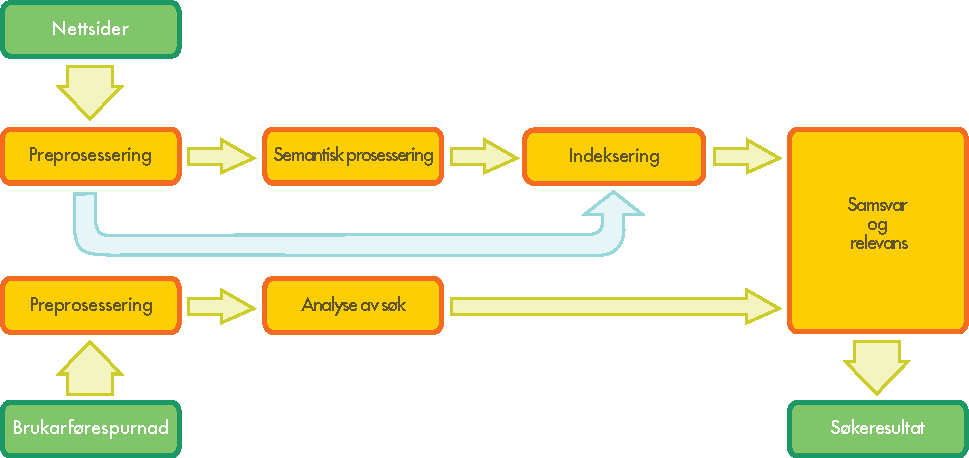
\includegraphics[width=\textwidth]{../_media/norwegian-nynorsk/web_search_architecture}
  \caption{Nettsøk}
  \label{fig:websearcharch_no}
  \colorrule{grey3}{\textwidth}{1.5pt}
 \end{figure*}

Digitale søk er sannsynlegvis den mest brukte språkteknologiske applikasjonen, men han er òg i stor grad underutvikla. Søkemotoren Google, som vart oppretta i 1998, utfører no om lag 80\% av alle nettsøk \cite{spi1}. 
Googles søkegrensesnitt og resultatvising har ikkje endra seg vesentleg sidan den første versjonen. Men i den noverande versjonen tilbyr Google stavekorrigering for feilstava ord, og har innarbeidt grunnleggjande semantiske søkemoglegheiter som kan betre nøyaktigheita gjennom analysar av tydinga til ordet i ein gjeven søkekontekst \cite{pc1}. Google sin suksess viser at med ei stor mengd tilgjengelege data kan ein statistisk orientert metode gje tilfredsstillande resultat. 

For meir sofistikerte informasjonssøk er det likevel avgjerande å integrere djupare lingvistiske analysar for teksttolking. Eksperiment med \textbf{leksikalske ressursar}, som maskinleselege tesaurusar eller ontologiske språkressursar (til dømes WordNet for engelsk, eit norsk ordnett er venta innan utgangen av 2012), har gjeve betre resultat når det gjeld å finne nettsider som inneheld synonym til den opphavlege søketermen, som
\textit{atomkraft}, \textit{kjerneenergi} og \textit{nukleærenergi}, og til og med termar som er endå lausare tilknytte.  

Den neste generasjonen søkemotorar må bruke ein mykje meir sofistikert språkteknologi, særleg for søk som består av eit spørsmål eller ein annan type setning, og ikkje berre ei liste av nøkkelord. For å svare på søket \textit{Gje meg ei liste over alle selskap som har vorte tekne over av eit anna selskap dei siste fem} må systemet gjere ein syntaktisk og \textbf{semantisk analyse} av setninga og lage eit hurtig oversyn over relevante dokument. Eit tilfredsstillande svar føreset ein syntaktisk analyse av den grammatiske strukturen til setninga for å slå fast at brukaren spør etter selskap som har vorte kjøpte opp, ikkje selskap som har kjøpt opp andre. Når det gjeld uttrykket \textit{dei siste fem åra}, må systemet avgjere kva for år det dreier seg om. Søket må så samanliknast mot ei stor mengd ustrukturerte data for å finne relevante treff. Dette blir kalla informasjonshenting (engelsk \textit{Information Retrieval}), og omfattar søk og rangering av relevante dokument. For å lage ei liste over selskapa treng systemet òg å forstå at ein viss ordstreng i eit dokument er namnet på eit selskap, ein prosess som blir kalla namneattkjenning. 

Ei endå større utfordring er å freiste å finne treff på eit søk i dokument på eit anna språk. Ved informasjonssøk på tvers av språk må søkeordet omsetjast automatisk til alle potensielle kjeldespråk, og resultata må deretter omsetjast tilbake til språka til brukaren. 

\boxtext{Den neste generasjonen søkemotorar må bruke ein mykje meir sofistikert språkteknologi.}

Sidan data i aukande grad blir oppbevart i andre format enn tekst,
trengst ei teneste for multimedial informasjonsinnhenting som lèt oss
søkje i bilete, lydfiler og videomateriale. Når det gjeld lyd- og
videofiler, må ein taleattkjenningsmodul konvertere taleinnhaldet til
tekst (eller fonetiske representasjonar) som så kan gje treff mot eit
brukarsøk. 

I Noreg utvikla Opera Software den første norske nettlesaren og Internettprogramvaren. Opera byrja i 1994 som eit forskingsprosjekt i Telenor. 
Etter eit år vart det skilt ut som eit uavhengig utviklingsselskap, Opera Software ASA. Nokre norske selskap utviklar eller appliserer søkeløysingar (CognIT, Comperio, TextUrgy, Abtrox og Infofinder). 
FAST utvikla ein søkemotor som vart kjøpt opp av Microsoft, og som no blir forhandla av Comperio. 
Utviklingsfokuset til desse selskapa er hovudsakleg retta mot å tilby tilleggsprogram og avanserte søkemotorar som utnyttar domenerelevant informasjon. 
IT-industrien i Noreg har altså allereie eit ganske godt grunnlag når det gjeld nettsøk og informasjonsinnhenting; det største behovet som føretaka rapporterer om, gjeld kvalitetssikra språkteknologiske komponentar.

\subsubsection{Taleteknologi}

Dei grunnleggjande taleteknologiane er taleattkjenning og talesyntese, som kan brukast til å utvikle til dømes taleinteraksjonsteknologi og dialogsystem. Taleteknologi blir brukt for å lage grensesnitt som lèt brukarane samhandle gjennom talespråk framfor å bruke ein grafisk skjerm, tastatur og mus. I dag blir talegrensesnitt brukt til heilt og delvis automatiserte telefontenester som selskap tilbyr kundane sine, tilsette eller partnarar. Talegrensesnitt blir brukt i stor grad til mellom anna banktenester, distribusjonskjeder, kollektivtransport og i telesektoren. Taleteknologi blir òg brukt til grensesnitt for navigasjonssystem i bilar og til bruk av talespråk som eit alternativ til grafiske grensesnitt eller trykkfølsame skjermar i smarttelefonar. 

\begin{figure*}[htb]
 \colorrule{grey3}{\textwidth}{1.5pt}
 \center
 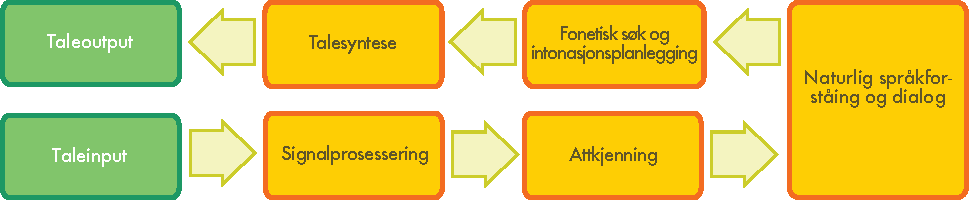
\includegraphics[width=\textwidth]{../_media/norwegian-nynorsk/simple_speech-based_dialogue_architecture}
 \caption{Talebasert dialogsystem}
 \label{fig:dialoguearch_no}
 \colorrule{grey3}{\textwidth}{1.5pt}
\end{figure*}

Taleteknologi omfattar fire typar verktøy: 

\begin{enumerate}
\item Automatisk \textbf{taleattkjenning} (tale-til-tekst) avgjer orda
  som faktisk blir sagde i ein gjeven lydsekvens ytra av ein
  språkbrukar.
\columnbreak

\item Naturleg språkforståing analyserer den syntaktiske strukturen i ytringa og tolkar ytringa ut frå systemet som blir brukt.
\item Dialogstyring avgjer kva for handling som skal utførast, gjeve ein bestemt brukarinput og ein viss systemfunksjonalitet.
\item \textbf{Talesyntese} (tekst-til-tale) omskaper svaret frå systemet til lydar som er forståelege for brukaren.
\end{enumerate}

Ei viktig utfordring for automatiske taleattkjenningssystem er å kjenne att orda som blir ytra. Utvalet av moglege ytringar må då enten avgrensast til eit knippe nøkkelord, eller at ein manuelt lagar språkmodellar som dekkjer eit stort omfang av naturlege språkytringar. Ved hjelp av maskinlæringsteknikkar kan ein òg automatisk generere språkmodellar frå \textbf{talekorpus}, dvs. store samlingar av tale i lydfiler og teksttranskripsjonar. Å avgrense ytringane inneber vanlegvis at brukarane blir pålagde å bruke grensesnittet på ein avgrensa måte, noko som kan svekkje aksepten til brukaren av verktøyet; på den andre sida vil det auke kostnadene monaleg å skape, fininnstille og vedlikehalde rike språkmodellar. Talegrensesnitt som bruker språkmodellar og lèt brukaren uttrykkje seg meir fleksibelt i byrjinga – ved hjelp av ein førespurnad som: \textit{Kva kan eg gjere for deg?} – er generelt automatisert og gjev ofte ei betre oppleving for brukarane.

\boxtext{Taleteknologi blir brukt til å lage grensesnitt som lèt brukarane samhandle gjennom talespråk heller enn å bruke ein grafisk skjerm, tastatur og mus.}

Føretak bruker ofte førehandsinnspelt tale, innspelt av profesjonelle for å generere materialet som skal brukast i talegrensesnitt. For statiske ytringar, der formuleringane ikkje avheng av ein viss situasjon eller personlege brukardata, kan dette gje ei god brukaroppleving. Men meir dynamisk ytringsinnhald kan pregast av unaturleg intonasjonsmønster fordi dei rett og slett blir produserte ved å lime ulike lydfiler saman. Dagens talesyntese har vorte stadig betre til å produsere dynamiske ytringar som høyrest naturlege ut, sjølv om dei framleis har eit forbetringspotensial. 

Det siste tiåret har det skjedd ei betydeleg standardisering av talegrensesnitt når det gjeld dei ulike teknologiske komponentane. Det har òg vore ei sterk marknadskonsolidering innan taleteknologi. I G20-landa (dei 19 landa i verda med best økonomi og dessutan EU) har berre fem globale aktørar dominert marknaden, med Nuance (USA) og Loquendo (Italia) som dei viktigaste i Europa. I 2011 kunngjorde Nuance oppkjøpet av Loquendo, og dette innebar eit nytt steg i retning av ei sterkare konsolidering av marknaden. 

For norsk talesyntese finst tretten norske stemmer; dei fleste har vorte utvikla av aktørane vi har nemnt ovanfor. 
Tre stemmer har vorte utvikla av det norske føretaket Lingit, som rettar seg mot brukarar med lese- og skrivevanskar. 
Ei anna stemme vart utvikla ved Norsk lyd- og blindeskriftbibliotek i samarbeid med søsterbiblioteket i Sverige. 
Der er òg ei aktiv forskargruppe ved NTNU i Trondheim. 

\boxtext{Språkressursar for talesyntese finst på engelsk, men berre i liten grad for norsk.}

Kvaliteten på talesyntese er sterkt avhengig av tilgjengelege ressursar (spesielt tekstkorpus tagga med informasjon om ordklasse, tokenisatorar og uttaleleksika) og språkspesifikk forsking på til dømes prosodiske trekk i det aktuelle språket. 
Det finst mange slike ressursar på engelsk, men berre i liten grad for norsk. Likevel er behovet ekstra stort for norsk på grunn av det store mangfaldet i moglege stavemåtar og dialektar, i tillegg til utfordringar knytte til tonelag og ein manglande éin-til-éin-relasjon mellom lydar og bokstavar. 

Når det gjeld teknologi og kunnskap for dialogstyring, er den norske marknaden dominert av mindre, norske føretak. 
MediaLT har utvikla ein generell taleattkjennar som blir til brukt til dialogstyring for blinde og svaksynte. 
Innan tale-til-tekst har Max Manus integrert og tilrettelagt Phillips’ SpeechMagic for norske sjukehus. 
Systemet er relativt vellukka, men har eit relativt avgrensa bruksområde med eit lukka vokabular. 
Nyleg vart Dragon Dictation, ein stemmeattkjenningsapplikasjon for mobiltelefonar, lansert for norsk. 
Denne applikasjonen er det første \textit{generelle} dikteringssystemet for norsk, men den norske versjonen av Dragon Dictation tolkar betydeleg meir feil enn den engelske versjonen. 
For taleinteraksjon finst det enno ikkje ein fungerande marknad for lingvistiske kjerneteknologiar for syntaktisk og semantisk analyse. 

Når ein ser framover, kan ein vente ei stor utvikling på grunn av større bruk av smarttelefonar som ei ny plattform for å handsame kunderelasjonar, i tillegg til eksisterande kommunikasjonsmedia som fasttelefonar, Internett og e-post. 
Dette vil sannsynlegvis òg påverke nytta av taleteknologi og dialogsystem. På sikt vil der sannsynlegvis bli færre telefonbaserte talegrensesnitt, og talespråksapplikasjonar vil spele ei langt meir sentral rolle som ein brukarvennleg interaksjonsmåte med smarttelefonar. 
Denne utviklinga vil sannsynlegvis primært drivast fram gjennom stegvise forbetringar av taleattkjenningssystem som ikkje er fokuserte på ein gjeven brukar, via dikteringssystem som alt blir tilbodne som sentraliserte tenester for smarttelefonbrukarar. 

\subsubsection{Maskinomsetjing}

\begin{figure*}[htb]
 \colorrule{grey3}{\textwidth}{1.5pt}
  \center
  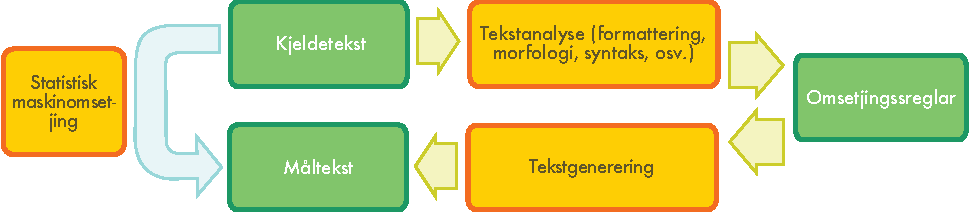
\includegraphics[width=\textwidth]{../_media/norwegian-nynorsk/machine_translation}
  \caption{Maskinomsetjing (venstre: statistisk; høgre: regelbasert)}
  \label{fig:mtarch_no}
  \colorrule{grey3}{\textwidth}{1.5pt}
\end{figure*}

Tanken om å bruke datamaskiner til å omsetje naturleg språk vart introdusert i 1946, og utløyste ein omfattande forskingsinnsats på 50-talet, som så vart gjenoppliva på 80-talet. Likevel har \textbf{maskinomsetjing} (MO) framleis ikkje levd opp til dei tidlege forhåpningane om å kunne tilby generell, automatisert omsetjing.

Den mest grunnleggjande tilnærminga til maskinomsetjing er automatisk å erstatte ord i eit språk med ord i eit anna språk. Dette kan fungere bra for domene der ordtilfanget er avgrensa og standardisert, som til dømes vêrmeldingar. Men for å lage gode omsetjingar av tekster frå meir generelle domene må ein omsetje større tekstbitar (ordgrupper, setningar, eller til og med heile avsnitt), og kvar tekstbit må vere i samsvar med tilsvarande del i kjeldeteksta. Maskinomsetjing er først og fremst vanskeleg fordi menneskeleg språk er fleirtydig. 

\boxtext{Maskinomsetjing er først og fremst vanskeleg fordi menneskeleg språk er fleirtydig.}

Fleirtydig språk gjev utfordringar på fleire nivå, mellom anna  kan ein ha bruk for å løyse det fleirtydige både på ordnivå og på setningsnivå. 
I ei enkel ord-for-ord-omsetjing til engelsk kan setninga \textit{Plutseleg rauk slangen} difor gje resultatet \textit{Suddenly smoked the snake.}
Verbforma \textit{rauk} (preteritum av \textit{ryke}) er fleirtydig mellom det vi på engelsk ville omsetje som høvesvis \textit{snap} og \textit{smoke}.
Orda \textit{slange} er på si side fleirtydig mellom `vasslange' (engelsk \textit{hose}) og `reptilslange' (engelsk \textit{snake}). Legg òg merke til at ei enkel ord-for-ord-omsetjing ikkje ville gjeve rett rekkjefølgje av orda på engelsk.

I tillegg til leksikalsk fleirtydigheit og skilnader i ordstilling kjem utfordringar med syntaktiske fleirtydigheiter. På norsk kan ein til dømes topikalisere objektet i ei setning, medan opninga for å gjere dette på engelsk er mykje meir avgrensa. Den norske setninga \textit{Epla åt mannen} har to ulike tolkingar: anten blir \textit{epla} analysert som subjektet til setninga (mannen vart eten av epla), eller som eit topikalisert objekt (epla vart etne av mannen). Sidan denne fleirtydigheita ikkje finst på engelsk, må eit maskinomsetjingssystem først finne den korrekte syntaktiske tolkinga for å kome fram til ei korrekt omsetjing.

Ei anna utfordring for maskinomsetjing for norsk er samansette ord. Eit effektivt omsetjingssystem må kunne identifisere samansette ord som ikkje står i ordboka, analysere dei, og om naudsynt lage nye samansette ord i målspråket.

For omsetjingar mellom språk som er nært i slekt kan ei enkel ord-for-ord-omsetjing la seg gjere. Men maskinomsetjingssystem kan òg byggjast ved å bruke lingvistiske reglar. Regelbaserte (eller kunnskapsdrivne) system analyserer kjeldeteksten, og lagar ein mellomståande symbolsk representasjon. På grunnlag av den symbolske representasjonen kan ein så generere tekst til målspråket. Kvaliteten på slike metodar avheng i stor grad av tilgangen til omfattande ordbøker med morfologisk, syntaktisk og semantisk informasjon, i tillegg til store sett med grammatiske reglar utvikla av språkforskarar. Dette er ein veldig omfattande, og difor dyr, prosess.

På slutten av 80-talet, då datamaskinkapasiteten auka, auka òg interessa for statistiske modellar for maskinomsetjing. Statistiske modellar for maskinomsetjing er basert på analysar av tospråklege tekstkorpus, som \textbf{parallellkorpuset} Europarl, som består av møtereferat frå Europaparlamentet på 11 europeiske språk 
(norsk er ikkje inkludert).
Viss ein har tilgang til tilstrekkelege mengder data, kan statistisk maskinomsetjing fungere godt nok til å finne den omtrentlege tydinga til ei tekst på eit anna språk, gjennom å prosessere parallelle versjonar av tekst og dermed finne sannsynlege ordmønster. Datadriven maskinomsetjing har sine fordelar, fordi ho krev mindre menneskeleg innsats, og kan fange opp særmerkte trekk ved språket (til dømes idiomatiske uttrykk) som kan oversjåast av kunnskapsdrivne system. Men i motsetnad til kunnskapsdrivne system gjev statistisk (eller datadrive) maskinomsetjing ofte ugrammatiske resultat.  

Ofte er det altså slik at fordelane og ulempene ved kunnskapsdriven og datadriven maskinomsetjing utfyller kvarandre. Difor fokuserer nyare forsking ofte på hybridtilnærmingar som kombinerer begge metodane. Ei slik tilnærming bruker både kunnskapsdrivne og datadrivne system saman med ein selekteringsmodul som avgjer det beste resultatet for kvar setning. For setningar lengre enn om lag tolv ord blir likevel resultata som regel mindre gode. Her kan ei betre løysing vere å kombinere dei beste delane frå kvar setning frå fleire ulike kjelder. Dette kan vere ei ganske kompleks oppgåve, sidan det ikkje alltid er klart kva for delar som passar saman. Desse må identifiserast og parallellstillast.   

\boxtext{Sjølv om det er eit klart behov for maskinomsetjing for norsk, er utviklinga av slik programvare for norsk enno ikkje omfattande.}

Når det gjeld omsetjing mellom dei to norske målformene, er behovet for effektive omsetjingsverktøy stort. To selskap har utvikla system for dette, Nynodata og Apertium. Nynodata er eit lite føretak som tilbyr verktøy for omsetjing, korrektur og tekstsøk for bokmål og nynorsk. Apertium er eit open-kjelde-initiativ som òg tilbyr automatisert omsetjing mellom dei to målformene, implementert av ein student ved Universitetet i Bergen.

Når det gjeld omsetjing mellom norsk og ulike framandspråk, har Google Translate ein norsk modul for omsetjing mellom engelsk og norsk; via engelsk er det mogleg å omsetje mellom norsk og kvart eit språkpar som inneheld engelsk. GramTrans er ei maskinomsetjingsplattform som er utvikla av det danske GrammarSoft ApS og det norske føretaket Kaldera Språkteknologi AS. Denne omsetjingsmotoren tilbyr ei teneste for gratis, nettbasert omsetjing for dei skandinaviske språka og mellom norsk og engelsk. Programmet er basert på ein robust grammatikkanalyse, ein transferkomponent som handsamar overgangen frå eitt språk til eit anna med omsyn til leksikon og grammatikk, og til slutt ein komponent som genererer omsett tekst på målspråket. Selskapet Clue Norge spesialiserer seg på elektroniske ordbøker for næringslivet, og utvikla for om lag ti år sidan systemet Textran for maskinomsetjing frå engelsk til norsk. Systemet eksisterer enno, men har ikkje vorte vidareutvikla fordi jamt pålitelege maskinomsetjingar av høg kvalitet er særs vanskeleg å oppnå, medan brukargruppene ikkje ynskte å betale for eit system som gjorde feil.

Sjølv om det føregår ein betydeleg forskingsinnsats på dette området, både nasjonalt og internasjonalt, har datadrivne og hybride system så langt vore mindre vellukka i applikasjonar for næringslivet enn i forskingslaboratoriet. I Noreg finst den viktigaste forskingsekspertisen ved Universitetet i Oslo og Universitetet i Bergen.

\boxtext{Språktenesteindustrien i Noreg har tilsynelatande eit underforbruk av språkteknologiske ressursar.}

Å bruke maskinomsetjing kan auke produktiviteten betydeleg, så lenge systemet er tilpassa brukarspesifikk terminologi og er godt integrert i arbeidsflyten på ein arbeidsplass. Generelt verkar det likevel som at språktenesteindustrien i Noreg har eit underforbruk av språkteknologiske ressursar. 
Sektoren kan delast i to grupper: på den eine sida har ein frilansomsetjarar og omsetjingsbyrå som rettar seg mot einskildpersonar, næringslivet og offentleg sektor; på den andre sida har ein omsetjarar som er knytte til Oversetterforeningen og Norsk faglitterær forfatter- og oversetterforening.

I den siste gruppa verker det som språkteknologi berre er i avgrensa bruk. Den førstnemnde gruppa bruker ofte Trados, som er det klart mest brukte omsetjingsverktøyet for profesjonelle omsetjarar. Trados har likevel ingen eigen modul for norsk, men støttar seg i staden på Hunspell, ei open-kjelde-løysing med stavekontroll og eit morfologisk analyseverktøy som opphavleg vart utvikla for ungarsk. Sjølv om det er ei funksjonell og open løysing, treng ho ytterlegare utvikling for å fungere som ein optimal ressurs for språktenestesektoren i Noreg. Særleg stort er behovet for å forbetre analysen av samansette ord på norsk. I tillegg bruker profesjonelle omsetjarar termbasar (DU, IATE), og til ein viss grad er der eit samarbeid med universitetssektoren i utviklinga av termbasar. Det tilsynelatande underforbruket av språkteknologiske ressursar i språktenesteindustrien heng delvis saman med mangelen på gode ressursar for norsk, men òg manglande kontakt mellom språktenesteleverandørar og forskarmiljøa. Difor kan kunnskap om det fulle potensialet for språkteknologi bli for avgrensa, og det kan vere vanskeleg for kommersielle aktørar å vurdere kvaliteten på eksisterande ressursar.

Kvaliteten på maskinomsetjingssystem har framleis eit stort forbetringspotensial. Blant utfordringane er å tilpasse språkressursar til eit gjeve emne eller brukarområde, og å integrere teknologien i ein arbeidsflyt som allereie inneheld termbasar og omsetjingsminne. I tillegg er dei fleste systema som er i bruk retta mot engelsk, og støttar berre sjeldan omsetjing til og frå norsk. Dette gjev forstyrringar i prosessen med å få tekst omsett, og tvingar maskinomsetjingsbrukarar til å lære seg ulike kodingsverktøy for ulike system.

\begin{figure*}[tb]
  \centering
  \setlength{\tabcolsep}{0.17em}
  \small
  \begin{tabular}{>{\columncolor{corange1}}cccccccccccccccccccccccc}
    & \multicolumn{22}{>{\columncolor{corange1}}c}{Målspråk -- \textcolor{grey1}{Target language}}\\\addlinespace[{-.009cm}]
    \rowcolor{corange1}  & EN & BG & DE & CS & DA & EL & ES & ET & FI & FR & HU & IT & LT & LV & MT & NL & PL & PT & RO & SK & SL & SV\\
    EN & -- & \textcolor{blue}{40.5} & \textcolor{blue}{46.8} & \textcolor{green2}{52.6} & \textcolor{green2}{50.0} & \textcolor{blue}{41.0} & \textcolor{green2}{55.2} & \textcolor{purple}{34.8} & \textcolor{purple}{38.6} & \textcolor{green2}{50.1} & \textcolor{purple}{37.2} & \textcolor{green2}{50.4} & \textcolor{purple}{39.6} & \textcolor{blue}{43.4} & \textcolor{purple}{39.8} & \textcolor{green2}{52.3} & \textcolor{blue}{49.2} & \textcolor{green2}{55.0} & \textcolor{blue}{49.0} & \textcolor{blue}{44.7} & \textcolor{green2}{50.7} & \textcolor{green2}{52.0}\\
    BG & \textcolor{green}{61.3} & -- & \textcolor{purple}{38.7} & \textcolor{purple}{39.4} & \textcolor{purple}{39.6} & \textcolor{purple}{34.5} & \textcolor{blue}{46.9} & \textcolor{red3}{25.5} & \textcolor{red3}{26.7} & \textcolor{blue}{42.4} & \textcolor{red3}{22.0} & \textcolor{blue}{43.5} & \textcolor{red3}{29.3} & \textcolor{red3}{29.1} & \textcolor{red3}{25.9} & \textcolor{blue}{44.9} & \textcolor{purple}{35.1} & \textcolor{blue}{45.9} & \textcolor{purple}{36.8} & \textcolor{purple}{34.1} & \textcolor{purple}{34.1} & \textcolor{purple}{39.9}\\
    DE & \textcolor{green2}{53.6} & \textcolor{red3}{26.3} & -- & \textcolor{purple}{35.4} & \textcolor{blue}{43.1} & \textcolor{purple}{32.8} & \textcolor{blue}{47.1} & \textcolor{red3}{26.7} & \textcolor{red3}{29.5} & \textcolor{purple}{39.4} & \textcolor{red3}{27.6} & \textcolor{blue}{42.7} & \textcolor{red3}{27.6} & \textcolor{purple}{30.3} & \textcolor{red2}{19.8} & \textcolor{green2}{50.2} & \textcolor{purple}{30.2} & \textcolor{blue}{44.1} & \textcolor{purple}{30.7} & \textcolor{red3}{29.4} & \textcolor{purple}{31.4} & \textcolor{blue}{41.2}\\
    CS & \textcolor{green2}{58.4} & \textcolor{purple}{32.0} & \textcolor{blue}{42.6} & -- & \textcolor{blue}{43.6} & \textcolor{purple}{34.6} & \textcolor{blue}{48.9} & \textcolor{purple}{30.7} & \textcolor{purple}{30.5} & \textcolor{blue}{41.6} & \textcolor{red3}{27.4} & \textcolor{blue}{44.3} & \textcolor{purple}{34.5} & \textcolor{purple}{35.8} & \textcolor{red3}{26.3} & \textcolor{blue}{46.5} & \textcolor{purple}{39.2} & \textcolor{blue}{45.7} & \textcolor{purple}{36.5} & \textcolor{blue}{43.6} & \textcolor{blue}{41.3} & \textcolor{blue}{42.9}\\
    DA & \textcolor{green2}{57.6} & \textcolor{red3}{28.7} & \textcolor{blue}{44.1} & \textcolor{purple}{35.7} & -- & \textcolor{purple}{34.3} & \textcolor{blue}{47.5} & \textcolor{red3}{27.8} & \textcolor{purple}{31.6} & \textcolor{blue}{41.3} & \textcolor{red3}{24.2} & \textcolor{blue}{43.8} & \textcolor{red3}{29.7} & \textcolor{purple}{32.9} & \textcolor{red3}{21.1} & \textcolor{blue}{48.5} & \textcolor{purple}{34.3} & \textcolor{blue}{45.4} & \textcolor{purple}{33.9} & \textcolor{purple}{33.0} & \textcolor{purple}{36.2} & \textcolor{blue}{47.2}\\
    EL & \textcolor{green2}{59.5} & \textcolor{purple}{32.4} & \textcolor{blue}{43.1} & \textcolor{purple}{37.7} & \textcolor{blue}{44.5} & -- & \textcolor{green2}{54.0} & \textcolor{red3}{26.5} & \textcolor{red3}{29.0} & \textcolor{blue}{48.3} & \textcolor{red3}{23.7} & \textcolor{blue}{49.6} & \textcolor{red3}{29.0} & \textcolor{purple}{32.6} & \textcolor{red3}{23.8} & \textcolor{blue}{48.9} & \textcolor{purple}{34.2} & \textcolor{green2}{52.5} & \textcolor{purple}{37.2} & \textcolor{purple}{33.1} & \textcolor{purple}{36.3} & \textcolor{blue}{43.3}\\
    ES & \textcolor{green}{60.0} & \textcolor{purple}{31.1} & \textcolor{blue}{42.7} & \textcolor{purple}{37.5} & \textcolor{blue}{44.4} & \textcolor{purple}{39.4} & -- & \textcolor{red3}{25.4} & \textcolor{red3}{28.5} & \textcolor{green2}{51.3} & \textcolor{red3}{24.0} & \textcolor{green2}{51.7} & \textcolor{red3}{26.8} & \textcolor{purple}{30.5} & \textcolor{red3}{24.6} & \textcolor{blue}{48.8} & \textcolor{purple}{33.9} & \textcolor{green2}{57.3} & \textcolor{purple}{38.1} & \textcolor{purple}{31.7} & \textcolor{purple}{33.9} & \textcolor{blue}{43.7}\\
    ET & \textcolor{green2}{52.0} & \textcolor{red3}{24.6} & \textcolor{purple}{37.3} & \textcolor{purple}{35.2} & \textcolor{purple}{37.8} & \textcolor{red3}{28.2} & \textcolor{blue}{40.4} & -- & \textcolor{purple}{37.7} & \textcolor{purple}{33.4} & \textcolor{purple}{30.9} & \textcolor{purple}{37.0} & \textcolor{purple}{35.0} & \textcolor{purple}{36.9} & \textcolor{red3}{20.5} & \textcolor{blue}{41.3} & \textcolor{purple}{32.0} & \textcolor{purple}{37.8} & \textcolor{red3}{28.0} & \textcolor{purple}{30.6} & \textcolor{purple}{32.9} & \textcolor{purple}{37.3}\\
    FI & \textcolor{blue}{49.3} & \textcolor{red3}{23.2} & \textcolor{purple}{36.0} & \textcolor{purple}{32.0} & \textcolor{purple}{37.9} & \textcolor{red3}{27.2} & \textcolor{purple}{39.7} & \textcolor{purple}{34.9} & -- & \textcolor{red3}{29.5} & \textcolor{red3}{27.2} & \textcolor{purple}{36.6} & \textcolor{purple}{30.5} & \textcolor{purple}{32.5} & \textcolor{red2}{19.4} & \textcolor{blue}{40.6} & \textcolor{red3}{28.8} & \textcolor{purple}{37.5} & \textcolor{red3}{26.5} & \textcolor{red3}{27.3} & \textcolor{red3}{28.2} & \textcolor{purple}{37.6}\\
    FR & \textcolor{green}{64.0} & \textcolor{purple}{34.5} & \textcolor{blue}{45.1} & \textcolor{purple}{39.5} & \textcolor{blue}{47.4} & \textcolor{blue}{42.8} & \textcolor{green}{60.9} & \textcolor{red3}{26.7} & \textcolor{purple}{30.0} & -- & \textcolor{red3}{25.5} & \textcolor{green2}{56.1} & \textcolor{red3}{28.3} & \textcolor{purple}{31.9} & \textcolor{red3}{25.3} & \textcolor{green2}{51.6} & \textcolor{purple}{35.7} & \textcolor{green}{61.0} & \textcolor{blue}{43.8} & \textcolor{purple}{33.1} & \textcolor{purple}{35.6} & \textcolor{blue}{45.8}\\
    HU & \textcolor{blue}{48.0} & \textcolor{red3}{24.7} & \textcolor{purple}{34.3} & \textcolor{purple}{30.0} & \textcolor{purple}{33.0} & \textcolor{red3}{25.5} & \textcolor{purple}{34.1} & \textcolor{red3}{29.6} & \textcolor{red3}{29.4} & \textcolor{purple}{30.7} & -- & \textcolor{purple}{33.5} & \textcolor{red3}{29.6} & \textcolor{purple}{31.9} & \textcolor{red2}{18.1} & \textcolor{purple}{36.1} & \textcolor{red3}{29.8} & \textcolor{purple}{34.2} & \textcolor{red3}{25.7} & \textcolor{red3}{25.6} & \textcolor{red3}{28.2} & \textcolor{purple}{30.5}\\
    IT & \textcolor{green}{61.0} & \textcolor{purple}{32.1} & \textcolor{blue}{44.3} & \textcolor{purple}{38.9} & \textcolor{blue}{45.8} & \textcolor{blue}{40.6} & \textcolor{red3}{26.9} & \textcolor{red3}{25.0} & \textcolor{red3}{29.7} & \textcolor{green2}{52.7} & \textcolor{red3}{24.2} & -- & \textcolor{red3}{29.4} & \textcolor{purple}{32.6} & \textcolor{red3}{24.6} & \textcolor{green2}{50.5} & \textcolor{purple}{35.2} & \textcolor{green2}{56.5} & \textcolor{purple}{39.3} & \textcolor{purple}{32.5} & \textcolor{purple}{34.7} & \textcolor{blue}{44.3}\\
    LT & \textcolor{green2}{51.8} & \textcolor{red3}{27.6} & \textcolor{purple}{33.9} & \textcolor{purple}{37.0} & \textcolor{purple}{36.8} & \textcolor{red3}{26.5} & \textcolor{red3}{21.1} & \textcolor{purple}{34.2} & \textcolor{purple}{32.0} & \textcolor{purple}{34.4} & \textcolor{red3}{28.5} & \textcolor{purple}{36.8} & -- & \textcolor{blue}{40.1} & \textcolor{red3}{22.2} & \textcolor{purple}{38.1} & \textcolor{purple}{31.6} & \textcolor{purple}{31.6} & \textcolor{red3}{29.3} & \textcolor{purple}{31.8} & \textcolor{purple}{35.3} & \textcolor{purple}{35.3}\\
    LV & \textcolor{green2}{54.0} & \textcolor{red3}{29.1} & \textcolor{purple}{35.0} & \textcolor{purple}{37.8} & \textcolor{purple}{38.5} & \textcolor{red3}{29.7} & \textcolor{red2}{8.0} & \textcolor{purple}{34.2} & \textcolor{purple}{32.4} & \textcolor{purple}{35.6} & \textcolor{red3}{29.3} & \textcolor{purple}{38.9} & \textcolor{purple}{38.4} & -- & \textcolor{red3}{23.3} & \textcolor{blue}{41.5} & \textcolor{purple}{34.4} & \textcolor{purple}{39.6} & \textcolor{purple}{31.0} & \textcolor{purple}{33.3} & \textcolor{purple}{37.1} & \textcolor{purple}{38.0}\\
    MT & \textcolor{green}{72.1} & \textcolor{purple}{32.2} & \textcolor{purple}{37.2} & \textcolor{purple}{37.9} & \textcolor{purple}{38.9} & \textcolor{purple}{33.7} & \textcolor{blue}{48.7} & \textcolor{red3}{26.9} & \textcolor{red3}{25.8} & \textcolor{blue}{42.4} & \textcolor{red3}{22.4} & \textcolor{blue}{43.7} & \textcolor{purple}{30.2} & \textcolor{purple}{33.2} & -- & \textcolor{blue}{44.0} & \textcolor{purple}{37.1} & \textcolor{blue}{45.9} & \textcolor{purple}{38.9} & \textcolor{purple}{35.8} & \textcolor{blue}{40.0} & \textcolor{blue}{41.6}\\
    NL & \textcolor{green2}{56.9} & \textcolor{red3}{29.3} & \textcolor{blue}{46.9} & \textcolor{purple}{37.0} & \textcolor{blue}{45.4} & \textcolor{purple}{35.3} & \textcolor{blue}{49.7} & \textcolor{red3}{27.5} & \textcolor{red3}{29.8} & \textcolor{blue}{43.4} & \textcolor{red3}{25.3} & \textcolor{blue}{44.5} & \textcolor{red3}{28.6} & \textcolor{purple}{31.7} & \textcolor{red3}{22.0} & -- & \textcolor{purple}{32.0} & \textcolor{blue}{47.7} & \textcolor{purple}{33.0} & \textcolor{purple}{30.1} & \textcolor{purple}{34.6} & \textcolor{blue}{43.6}\\
    PL & \textcolor{green}{60.8} & \textcolor{purple}{31.5} & \textcolor{blue}{40.2} & \textcolor{blue}{44.2} & \textcolor{blue}{42.1} & \textcolor{purple}{34.2} & \textcolor{blue}{46.2} & \textcolor{red3}{29.2} & \textcolor{red3}{29.0} & \textcolor{blue}{40.0} & \textcolor{red3}{24.5} & \textcolor{blue}{43.2} & \textcolor{purple}{33.2} & \textcolor{purple}{35.6} & \textcolor{red3}{27.9} & \textcolor{blue}{44.8} & -- & \textcolor{blue}{44.1} & \textcolor{purple}{38.2} & \textcolor{purple}{38.2} & \textcolor{purple}{39.8} & \textcolor{blue}{42.1}\\
    PT & \textcolor{green}{60.7} & \textcolor{purple}{31.4} & \textcolor{blue}{42.9} & \textcolor{purple}{38.4} & \textcolor{blue}{42.8} & \textcolor{blue}{40.2} & \textcolor{green}{60.7} & \textcolor{red3}{26.4} & \textcolor{red3}{29.2} & \textcolor{green2}{53.2} & \textcolor{red3}{23.8} & \textcolor{green2}{52.8} & \textcolor{red3}{28.0} & \textcolor{purple}{31.5} & \textcolor{red3}{24.8} & \textcolor{blue}{49.3} & \textcolor{purple}{34.5} & -- & \textcolor{purple}{39.4} & \textcolor{purple}{32.1} & \textcolor{purple}{34.4} & \textcolor{blue}{43.9}\\
    RO & \textcolor{green}{60.8} & \textcolor{purple}{33.1} & \textcolor{purple}{38.5} & \textcolor{purple}{37.8} & \textcolor{blue}{40.3} & \textcolor{purple}{35.6} & \textcolor{green2}{50.4} & \textcolor{red3}{24.6} & \textcolor{red3}{26.2} & \textcolor{blue}{46.5} & \textcolor{red3}{25.0} & \textcolor{blue}{44.8} & \textcolor{red3}{28.4} & \textcolor{red3}{29.9} & \textcolor{red3}{28.7} & \textcolor{blue}{43.0} & \textcolor{purple}{35.8} & \textcolor{blue}{48.5} & -- & \textcolor{purple}{31.5} & \textcolor{purple}{35.1} & \textcolor{purple}{39.4}\\
    SK & \textcolor{green}{60.8} & \textcolor{purple}{32.6} & \textcolor{purple}{39.4} & \textcolor{blue}{48.1} & \textcolor{blue}{41.0} & \textcolor{purple}{33.3} & \textcolor{blue}{46.2} & \textcolor{red3}{29.8} & \textcolor{red3}{28.4} & \textcolor{purple}{39.4} & \textcolor{red3}{27.4} & \textcolor{blue}{41.8} & \textcolor{purple}{33.8} & \textcolor{purple}{36.7} & \textcolor{red3}{28.5} & \textcolor{blue}{44.4} & \textcolor{purple}{39.0} & \textcolor{blue}{43.3} & \textcolor{purple}{35.3} & -- & \textcolor{blue}{42.6} & \textcolor{blue}{41.8}\\
    SL & \textcolor{green}{61.0} & \textcolor{purple}{33.1} & \textcolor{purple}{37.9} & \textcolor{blue}{43.5} & \textcolor{blue}{42.6} & \textcolor{purple}{34.0} & \textcolor{blue}{47.0} & \textcolor{purple}{31.1} & \textcolor{red3}{28.8} & \textcolor{purple}{38.2} & \textcolor{red3}{25.7} & \textcolor{blue}{42.3} & \textcolor{purple}{34.6} & \textcolor{purple}{37.3} & \textcolor{purple}{30.0} & \textcolor{blue}{45.9} & \textcolor{purple}{38.2} & \textcolor{blue}{44.1} & \textcolor{purple}{35.8} & \textcolor{purple}{38.9} & -- & \textcolor{blue}{42.7}\\
    SV & \textcolor{green2}{58.5} & \textcolor{red3}{26.9} & \textcolor{blue}{41.0} & \textcolor{purple}{35.6} & \textcolor{blue}{46.6} & \textcolor{purple}{33.3} & \textcolor{blue}{46.6} & \textcolor{red3}{27.4} & \textcolor{purple}{30.9} & \textcolor{purple}{38.9} & \textcolor{red3}{22.7} & \textcolor{blue}{42.0} & \textcolor{red3}{28.2} & \textcolor{purple}{31.0} & \textcolor{red3}{23.7} & \textcolor{blue}{45.6} & \textcolor{purple}{32.2} & \textcolor{blue}{44.2} & \textcolor{purple}{32.7} & \textcolor{purple}{31.3} & \textcolor{purple}{33.5} & --\\
    \end{tabular}
  \caption{Maskinomsetjing mellom 22 EU-språk -- \textcolor{grey1}{Machine translation between 22 EU-languages \cite{euro1}}}
  \label{fig:euromatrix_de}
\end{figure*}


Gjennom evalueringskampanjar samanliknar forskarar kvaliteten på ulike maskinomsetjingssystem og tilnærmingar og ikkje minst kva som er status for systema for ulike språkpar.
%start Norwegian
Prosjektet EuroMatrix+ gjennomførde ein studie av kvaliteten på maskinomsetjingssystem for 22 offisielle EU-språk. Norsk var ikkje inkludert i dette prosjektet.
Figur~\ref{fig:euromatrix_de} (s.~\pageref{fig:euromatrix_de}), som vart laga gjennom prosjektet EuroMatrix+, viser ei parvis samanlikning av resultata for 22 av dei 23 EU-språka (irsk var ikkje med i samanlikninga). Resultata er rangert med bruk av BLEU-poenggjeving, som gjev høgare poeng for betre omsetjingar \cite{bleu1}. Ein menneskeleg omsetjar ville vanlegvis oppnå rundt 80 poeng. Dei resultata (i grønt og blått) fann ein med språk som nyt godt av omfattande forskingsinnsats innanfor koordinerte forskingsprogram og som har mange parallellkorpus (t.d. engelsk, fransk, nederlandsk, spansk og tysk). Språka med lavare poengsum er viste i raudt. Desse språka manglar anten heilt ein velutvikla forskingsinnsats eller så skil dei seg strukturelt veldig frå andre språk (t.d. ungarsk, maltisk, finsk).  
%end Norwegian

\subsection{Andre bruksområde}

Oppbygginga av språkteknologiske verktøy omfattar ei rekkje underoppgåver som ikkje alltid er synlege på overflata, der kommunikasjonen med brukaren skjer. Slike underliggjande program har likevel viktige funksjonar i systemet. Kvar av oppgåvene utgjer viktige forskingsfelt, som har utvikla seg til enkeltdisiplinar innanfor datalingvistikk. 

Såkalla dialogsystem som svarer på spørsmål (engelsk \textit{Question Answering}) er til dømes eit aktivt forskingsområde, der ein har utvikla korpus koda med setningsstruktur, og der vitskaplege evalueringskonkurransar har vore initierte. Feltet omfattar meir enn berre søk på nøkkelord (der søkemotoren svarar med ei samling potensielt relevante dokument); det lèt brukarar stille konkrete spørsmål som systemet så gjev eitt einaste svar på. Til dømes:
\begin{itemize}
\item[] \textit{Spørsmål: Kor gammal var Neil Armstrong då han gjekk på månen?}
\item[] \textit{Svar: 38.}
\end{itemize}

Medan slike dialogsystem openbert er relaterte til nettsøk, blir det i dag nytta som eit overordna omgrep for forskingsspørsmål som kva for typar spørsmål som finst, korleis ein skal handsame dei, korleis ein kan analysere og samanlikne sett av dokument som potensielt inneheld svaret (gjev dokumenta til dømes motstridande svar?), og korleis relevant informasjon kan ekstraherast frå eit dokument med minimal grad av feil, og utan å sjå bort frå kontekst. Dette er i sin tur knytt til informasjonsekstrahering (engelsk \textit{Information Extraction}), eit område som vart svært populært og innflytelsesrikt då datalingvistikken vart meir statistisk orientert tidleg på 90-talet. Informasjonsekstrahering har som mål å finne bestemte bitar av informasjon i visse sett av dokument, til dømes å identifisere dei viktigaste aktørane i avisartiklar som handlar om å ta over føretak. Eit anna scenario som kan studerast, er terrorhandlingar. Problemstillinga er då å sortere informasjon i teksten i samsvar med ein førehandsdefinert mal som spesifiserer kriterium som gjerningsmann, mål, tid, stad og utfall av hendinga. Informasjonsekstrahering består grunnleggjande sett i å fylle ut ein mal med domenespesifikk og relevant informasjon, noko som gjer informasjonsekstrahering til nok eit døme på ein underliggjande teknologi som på den eine sida utgjer eit sjølvstendig forskingsfelt, og som på den andre sida skal kunne integrerast i større brukarapplikasjonar for praktisk nytte.

\boxtext{Forsking på dei fleste typar tekstteknologi er langt mindre utvikla for norsk enn for engelsk.}

Samandrag og \textbf{tekstgenerering} er tilgrensande område som kan brukast som sjølvstendige applikasjonar eller som underliggjande støtteteknologi. Samandrag har som mål å gje att dei viktigaste punkta i ei lengre tekst, og finst mellom anna  i Microsoft Word. Oftast blir det brukt ei statistisk tilnærming for å identifisere dei `viktige' orda i ei tekst (dvs. ord som opptrer hyppig i den aktuelle teksta, men meir sjeldan i allmennspråket) og for å finne dei setningane som har høgast førekomst av desse `viktige' orda. Dei aktuelle setningane blir så trekte ut og sette saman for å lage eit samandrag. I ein slik modell, som er svært utbreidd i kommersiell nytte, er samandrag rett og slett ei form for ekstrahering av setningar, og teksta blir redusert til eit subsett av setningane sine. Eit anna alternativ er å generere heilt nye setningar som ikkje allereie finst i kjeldeteksten, og ein del forsking blir gjort på dette feltet.

Å generere nye setningar som oppsummerer originaltekst krev ei djupare forståing av teksta, og denne tilnærminga er difor så langt betydeleg mindre robust. Generelt blir ein tekstgenerator sjeldan brukt som ein sjølvstendig applikasjon, men blir i staden integrert i eit større programvaremiljø, som til dømes eit informasjonssystem om kliniske data som samlar, lagrar og prosesserer pasientopplysningar. Rapportgenerering er berre eitt av mange potensielle bruksområde for samandrag.
I USA har det sidan 90-talet vore fleire opne konkurransar i å svare på spørsmål automatisk eller dialogsystem, informasjonsekstrahering og samandrag, som først og fremst har vore arrangert av dei offentlege støtta organisasjonane DARPA og NIST. Gjennom desse konkurransane har teknologien vorte klart forbetra, men hovudfokus har altså vore på engelsk. 
Det finst nesten ikkje annoterte korpus eller andre spesialressursar for å utføre slike oppgåver på norsk. 
Når tekstoppsummeringssystem utelukkande bruker statistiske metodar, er dei i høg grad språkuavhengige, og det finst mange tilgjengelege forskingsprototypar. 
For tekstgenerering har komponentar som kan brukast om att stort sett vore avgrensa til modular for produksjon av overflatestrukturen, og det meste av tilgjengeleg programvare er for engelsk. 

\subsection{Utdanningsprogram}

Språkteknologi er eit interdisiplinært fagfelt som samlar ekspertise frå bl.a. språkforsking, informatikk, matematikk, filosofi, psykolingvistikk og nevrovitskap.
Difor har ikkje språkteknologi fått etablert ein klart definert, sjølvstendig plass i det norske universitetssystemet. 

\boxtext{Språkteknologi har ikkje ein klart definert, sjølvstendig plass i det norske universitetssystemet.}

I Noreg finst den språkvitskaplege ekspertisen i mindre forskargrupper ved ulike institusjonar som samarbeider på prosjektbasis (Universiteta i Oslo, Bergen og Tromsø, NTNU, NHH og forskingsinstitusjonane Uni Research og Sintef). Ingen av universiteta har eigne institutt eller senter for datalingvistikk. Undervising i datalingvistikk føregår anten ved institutt for informatikk (Universitetet i Oslo og NTNU) eller lingvistikk (Universiteta i Bergen og Tromsø). Forsking og undervising i taleprosessering føregår berre ved NTNU.

Sjølv om det er vanskeleg å kvantifisere ein slik påstand, er det nok rimeleg å hevde at datalingvistikk og språkteknologi, så vel som høva for å studere dette i Noreg, ikkje er særleg godt kjend i Noreg. Eit viktig mål for KUNSTI-programmet var å styrkje grunnforsking og kompetansen innanfor dei språkteknologiske fagfelta. KUNSTI bidrog til fleire masteroppgåver og doktoravhandlingar innanfor ei rekkje forskingsprosjekt. Forskingsprogrammet spelte dermed ei viktig rolle for å skaffe norsk språkteknologi nye forskarar og auka kompetanse. Universitetet i Bergen koordinerer CLARA, eit nettverk for forskarutdanning innan SRT ved ni europeiske institusjonar.

\subsection{Nasjonale prosjekt og initiativ}

Sidan norsk språkteknologisk industri er relativt liten i internasjonal samanheng, har norske forskingsinstitusjonar spelt ei sentral rolle i utviklinga av norske ressursar og verktøy for språkteknologi, noko som òg har kome private føretak til nytte. 
Dei fleste norske selskap som treng språkteknologi vil gjerne nyttiggjere seg ressursar, kunnskap og ekspertise frå akademia, fordi deira eigen ekspertise vanlegvis ikkje ligg innanfor språkteknologi. 

Noregs forskingsråd har så langt støtta eitt betydeleg språkteknologisk forskingsprogram, nemleg KUNSTI (Kunnskapsutvikling for norsk språkteknologi). 
Dette programmet var delvis inspirert av større prosjekt i andre land (til dømes det tyske prosjektet Verbmobil), og hadde som mål å auke kompetansen om språkteknologi gjennom grunnforsking. KUNSTI skulle gjere skriftleg og munnleg norsk (og til ein viss grad samisk) tilgjengeleg for databehandling gjennom forsking og utvikling. Tjue forskingsprosjekt av ulike storleikar vart gjennomførde i løpet av programperioden; dei to største var innan maskinomsetjing og taleteknologi.

\boxtext{Språkbanken er ei av dei viktegaste språkpolitiske satsingane vi har hatt i Noreg i nyare tid.}

Å byggje opp eit mangfald av språkteknologiske applikasjonar føreset tilgjenge på grunnleggjande ressursar, som ordlister, tekstkorpus og talekorpus. Slike ressursar er like dyre og tidkrevjande å utvikle for små språk som for store; sidan norsk har to offisielle målformer blir kostnadene endå høgare. 
Difor er ikkje norsk så interessant frå ein kommersiell ståstad. Difor var det eit viktig språkpolitisk tiltak at Språkbanken vart oppretta i 2010, etter tjue år med felles innsats frå Språkrådet, Noregs forskingsråd, næringslivet og norske forskingsinstitusjonar. Språkbanken ved Nasjonalbiblioteket skal fungere som ein infrastruktur for å gjere norsk språkteknologi tilgjengeleg både for forsking og kommersiell utvikling, noko som vonleg vil senke terskelen for å utvikle nye språkteknologiske produkt for norsk. 

Så langt har private selskap typisk bygd ulike ressursar og verktøy til intern bruk, medan dei fleste omfattande (og tilgjengelege) ressursar og verktøy (til dømes leksikon, taggarar og namneattkjennarar) er utvikla ved forskingsinstitusjonane. På eit seinare tidspunkt har desse ressursane i nokre tilfelle vorte kjøpte av private føretak. Faktisk inneheld tabellen over verktøy og ressursar i slutten av denne rapporten hovudsakleg ressursar som er utvikla gjennom forsking. Til dømes har Universitetet i Oslo utvikla talekorpuset Nota-Oslo (Norsk Talespråkskorpus, Oslo-delen) og Nordisk dialektkorpus, Norsk ordbank er utvikla og er ått av Universitetet i Oslo og Norsk språkråd, Oslo-Bergen-taggaren er laga av Universitetet i Oslo og Uni Research i Bergen, Norsk aviskorpus er utvikla av Uni Research og NHH, og trebanken INESS blir for tida bygd opp ved Universitetet i Bergen.

Utvikling av grunnleggjande tekst- og taledata var ikkje ein del av Kunstis arbeidsprogram, sidan dette skulle vere ei oppgåve for Språkbanken. Mangelen på grunnleggjande språkressursar stod dermed fram som ein hemsko for KUNSTI. No som Språkbanken er etablert, og med nye forskarar og oppdatert kompetanse på plass, meiner mange at tida er moden for ei ny satsing på språkteknologisk forsking som kan få eit meir applikasjonsorientert fokus enn KUNSTI-satsinga. Etter KUNSTI har større språkteknologiske forskingsprosjekt (til dømes INESS, Nota-Oslo, Norsk aviskorpus, WeSearch-Språkteknologi for internett og SIRKUS) vorte finansierte anten gjennom infrastrukturprogramma (AVIT) eller forskingsrådets generelle IKT-program, som VERDIKT. 
%Som eit ledd i arbeidet med å byggje opp ein norsk infrastruktur for språkressursar inngjekk Språkbanken i 2011 ein avtale med Kaldera språkteknologi AS om å byggje eit ordnett for bokmål og nynorsk. 
Trass i desse investeringane er likevel støtta til språkteknologiske prosjekt i Noreg relativt låg samanlikna med det som blir brukt til dømes i USA på omsetjing og fleirspråkleg informasjonstilgang \cite{laz1}.

%Som ei oppsummering har dette delkapitlet vist at tidlegare forskingsprogram har ført til ei utvikling av ei rekkje språkteknologiske verktøy og ressursar for norsk språk. 
I neste delkapittel oppsummerer vi situasjonen for språkteknologisk støtte for norsk språk. 

\subsection{Situasjonen for språkteknologisk støtte for norsk språk}

%Numbers have been inserted, but it would be good to go over them
\begin{figure*}[htb]
\centering
%\begin{tabular}{>{\columncolor{orange1}}p{.33\linewidth}ccccccc} % ORIGINAL
\begin{tabular}{>{\columncolor{orange1}}p{.33\linewidth}@{\hspace{6mm}}c@{\hspace{6mm}}c@{\hspace{6mm}}c@{\hspace{6mm}}c@{\hspace{6mm}}c@{\hspace{6mm}}c@{\hspace{6mm}}c}
\rowcolor{orange1}
 \cellcolor{white}&\begin{sideways}\makecell[l]{Kvantitet}\end{sideways}
&\begin{sideways}\makecell[l]{\makecell[l]{Tilgjengelegheit} }\end{sideways} &\begin{sideways}\makecell[l]{Kvalitet}\end{sideways}
&\begin{sideways}\makecell[l]{Dekningsgrad}\end{sideways} &\begin{sideways}\makecell[l]{Modenheit}\end{sideways} &\begin{sideways}\makecell[l]{Berekraft}\end{sideways} &\begin{sideways}\makecell[l]{Tilpassingsdyktigheit~~~}\end{sideways} \\ \addlinespace
\multicolumn{8}{>{\columncolor{orange2}}l}{Språkteknologi (verktøy, teknologiar og applikasjonar)} \\ \addlinespace
Taleattkjenning &4&2&2&1&2&3&3 \\ \addlinespace
Talesyntese &3&2&3&2&3&3&3\\ \addlinespace
Grammatisk analyse &4&4,5&4&4&4,5&4,5&5\\ \addlinespace
Semantisk analyse &2&2&3,3&3&3,7&3,3&3,7\\ \addlinespace
Tekstgenerering &1&4&4&3&5&4&5\\ \addlinespace
Maskinomsetjing &4&4&2&2&3&5&3\\ \addlinespace
\multicolumn{8}{>{\columncolor{orange2}}l}{Språkressursar (ressurs-, data- og kunnskapsbasar)} \\ \addlinespace
Tekstkorpus &4,5&3,5&3,5&3&4&4,5&4\\ \addlinespace
Talekorpus &5&4&3&5&4&5&5\\ \addlinespace
Parallellkorpus &5&3&2&2&4&3&3\\ \addlinespace
Leksikalske ressursar &2,5&2&2&2&2&2&2,5\\ \addlinespace
Grammatikkar &2&4&5&3&4&5&3\\
\end{tabular}
\caption{Status for SRT for norsk}
\label{fig:lrlttable_no}
\end{figure*}

Figur~\ref{fig:lrlttable_no} oppsummerer situasjonen for språkteknologisk støtte for norsk språk gjennom talvurderingar av eksisterande verktøy og ressursar. Vurderingane er gjorde av leiande norske ekspertar på feltet, som har sett talverdiar for sju ulike kriterium (t.d. tilgjenge), på ein skala frå 0 (svært låg) til 6 (svært høg). 
Dei viktigaste resultata for norsk kan oppsummerast slik: 

\begin{itemize}
\item Situasjonen for norsk er relativt god når det gjeld dei mest grunnleggjande språkteknologiske verktøya og ressursane, som taggarar, morfologisk analyse, referansekorpus og talekorpus.
Det finst òg mange talesynteseprodukt for norsk som er generelt
brukande og som har ein akseptabel kvalitet, sjølv om dei fleste av
dei er utvikla av kommersielle aktørar, og dermed har avgrensa
tilgjenge. Der finst fleire leksikalske ressursar som dekkjer
allmennspråket, men der er betydelege manglar når det gjeld
terminologi for spesialiserte domene.

\smallskip
\item Det finst òg ressursar og verktøy med avgrensa funksjonalitet
  innan felt som taleattkjenning, maskinomsetjing og
  teksttolking. Nokre av desse områda blir likevel dekte hovudsakleg
  av kommersielle aktørar, og har dermed avgrensa tilgjenge.

\smallskip
\item For enkelte typar verktøy og ressursar finst nesten ingen ressursar, medan andre ressursar er utvikla for kommersielle føremål og er ikkje allment tilgjengelege. 
Dette gjeld til dømes verktøy og ressursar for meir avansert
språkteknologi for norsk, som avansert diskursprosessering,
tekstgenerering og ontologiar som representerer verdskunnskap.

\smallskip
\item Mange verktøy og ressursar manglar standardisering, det vil seie at sjølv om dei eksisterer, er dei ikkje nødvendigvis i standardformat som sikrar at dei er, og blir verande, brukande og enkle å tilpasse nye bruksområde.
Sjølv om tabellen viser at grunnleggjande verktøy og ressursar finst for norsk, er dei i nokre tilfelle fragmenterte, og nytteverdien er avgrensa av restriksjonar på bruk, inkompatibilitet med andre system og manglande dokumentasjon. 
\end{itemize}

\medskip 
Kort oppsummert har vi i dag tilgjengelege ressursar og verktøy med avgrensa funksjonalitet på ei rekkje felt for norsk språkteknologi.
Det er heilt tydeleg naudsynt med ei ytterlegare satsing for å rette opp dei noverande manglane med omsyn til djupare semantisk prosessering av språk og for å produsere fleire ressursar, som parallelle korpus for maskinomsetjing.

\subsection{Samanlikning på tvers av språk}

Situasjonen for språkteknologi varierer mykje frå språk til språk. For å samanlikne situasjonen for ulike språk presenterer vi i dette delkapitlet ei vurdering basert på to utvalde applikasjonsområde (maskinomsetjing og taleprosessering), ein underliggjande teknologi (tekstanalyse), og grunnleggjande ressursar som trengst for å byggje språkteknologiske applikasjonar. Språka vart delte inn på ein skala med fem kategoriar:

\begin{enumerate}
\item Framifrå støtte
\item God støtte
\item Middels god støtte 
\item Fragmentarisk støtte
\item Låg eller inga støtte
\end{enumerate}

Den språkteknologiske støtta vart målt ut frå følgjande kriterium:

\textbf{Taleprosessering:} Kvaliteten til eksisterande taleattkjenning, kvaliteten til eksisterande talesyntese, dekning av ulike domene, mengda og omfanget av eksisterande talekorpus, mengda og spreiinga av tilgjengelege talebaserte applikasjonar.

\textbf{Maskinomsetjing:} Kvaliteten til eksisterande omsetjingsteknologiar, mengda språkpar, dekninga for språklege konstruksjonar og domene, og kvaliteten til, og omfanget av, tilgjengelege system.

\textbf{Tekstanalyse:} Kvaliteten til, og dekningsgraden av, eksisterande teknologiar for tekstanalyse (morfologisk, syntaktisk, semantisk), dekninga av språklege konstruksjonar og domene, mengda og omfanget av eksisterande (annoterte) korpus, kvaliteten og dekningsgraden for eksisterande leksikalske ressursar (t.d. ordnett) og grammatikkar.

\textbf{Ressursar:} Kvaliteten og omfanget av eksisterande tekstkorpus, talekorpus og parallelle korpus, kvaliteten og dekningsgraden for eksisterande leksikalske ressursar og grammatikkar.

\boxtext{Undersøkinga vår viser tydeleg at språkteknologiske ressursar og verktøy for norsk enno ikkje har same kvalitet og dekningsgrad som ressursar og verktøy ein kan samanlikne med for engelsk.}

Figurane~\ref{fig:speech_cluster_no} til~\ref{fig:resources_cluster_no} viser tydeleg at språkteknologiske ressursar og verktøy for norsk enno ikkje har same kvalitet og dekningsgrad som ressursar og verktøy ein kan samanlikne med for engelsk. 

Men sjølv for dette språket som ligg på toppen, er det enno manglar når det gjeld høgkvalitetsapplikasjonar. 
Den norske situasjonen er godt i samsvar med nabolanda, sjølv om tala ikkje viser skilnadene som finst mellom bokmål og nynorsk.

Fleire norsktalande stemmer for talesyntese er tilgjengelege i ulike sluttbrukarapplikasjonar, men dei vanlege operativsystema tilbyr ikkje norsk talesyntese som kan brukast av utviklarar. 

For taleattkjenning er det lita støtte for norsk, og det finst ingen generelle taleattkjennarar, med eit mogleg unntak av Dragon Dictation, ein ny mobilapplikasjon som ikkje var tilgjengeleg i tide til å bli vurdert i denne rapporten.
Det finst eitt spesialisert dikteringsverktøy for helsevesenet med varierande kvalitet.

For maskinomsetjing mellom norsk bokmål og nynorsk finst det eitt tovegs, fritt tilgjengeleg program og eitt einvegs, kommersielt program. 
For maskinomsetjing mellom norsk og andre språk finst det eitt gratis, fritt tilgjengeleg program og eitt kommersielt program. Begge har varierande kvalitet og yting.

Komponentar for tekstanalyse dekkjer det norske språket til ein viss grad, og inngår i fleire applikasjonar som typisk gjennomfører ein nokså overflatisk språkanalyse, t.d. generelle stavekontrollar eller skrivestøtte for dyslektikarar.

Med omsyn til ressursar har vi allereie peikt på manglar.
For å byggje meir avanserte program, til dømes maskinomsetjing, er det eit tydeleg behov for ressursar og verktøy som dekkjer eit breiare utval av språklege fenomen og som utfører ein djupare semantisk analyse. Betre kvalitet og dekningsgrad vil kunne takle eit breitt spekter av avanserte bruksområde, mellom anna  generell maskinomsetjing av høg kvalitet.

\subsection{Oppsummering}

\emph{Denne kvitbokserien er meint som eit viktig første tiltak for å vurdere situasjonen for språkteknologi for 30 europeiske språk, og å gje ei overordna samanlikning på tvers av språka. Gjennom denne analysen av manglar og behov er det europeiske språkteknologimiljøet og andre interesserte no i stand til å utvikle eit forskings- og utviklingsprogram i stor skala, der målet er å byggje eit verkeleg fleirspråkleg Europa basert på moderne språkteknologi.}

Vi har sett at det er store skilnader frå språk til språk. Medan det finst programvare og ressursar av høg kvalitet for enkelte språk og bruksområde, er det betydelege manglar for andre (vanlegvis `mindre') språk og bruksområde. Mange språk manglar grunnleggjande verktøy for tekstanalyse og grunnlagsressursane som trengst for å utvikle dei. Andre språk har grunnleggjande verktøy og ressursar, men er enno ikkje i stand til å investere i utviklinga av semantisk prosessering og analyse. Vi treng difor ein storstilt innsats om vi skal nå målet om å kunne tilby teknologistøtte av høg kvalitet til alle dei europeiske språka, t.d. maskinomsetjing av god kvalitet.

Når det gjeld norsk, har vi sett at det ikkje er enkelt å overføre teknologi som er utvikla og optimalisert for det engelske språket. 
Det kostar like mykje å utvikle språkressursar for eit lite språk som for eit større språk. Det er difor viktig med ei stabil og føreseieleg offentleg støtte til FoU for norsk språkteknologi, ikkje minst sidan norsk har to målformer. 
Vi har enno ikkje nådd det investeringsnivået som trengst. Den delen av språkteknologibransjen i Noreg som driv med teknologioverføring og kommersialisering er i dag ganske fragmentert. Aktørane er stort sett spesialiserte, små og mellomstore føretak som ikkje er robuste nok til å overleve og vekse på den nasjonale og den internasjonale marknaden.

Meir spesifikt kan dei mest presserande behova for norsk språkteknologi oppsummerast slik:
\begin{enumerate}
\item Betre lisensieringsvilkår og standardisering av eksisterande basisressursar og -verktøy for å gjere desse ope tilgjengelege for forsking og utvikling.
\item Utvikling av manglande basisressursar og -verktøy, mellom anna  fleirspråklege ressursar og verktøy med norsk som kjelde- eller målspråk, i standardformat og med opne lisensar.
\item Grunnforsking på avanserte automatiske språklege analysar for norsk og på integrering av statistisk og regelbasert språkteknologi, ikkje minst for å satse på ei tettare integrering av tale- og tekstteknologi.
\item Samordna formidling og utveksling av forskingsresultat for å synleggjere dei betre overfor potensielle brukarar, og for å trekkje nye forskarar og studentar til feltet.
\item Langsiktige og føreseielege finansieringsordningar for å sikre utvikling av språkteknologi, både for dei to norske målformene og for minoritetsspråk.
\end{enumerate}

For eit lite språksamfunn som norsk, med eit lite forskingsmiljø, er samarbeid viktig, ikkje berre på nasjonalt nivå men òg internasjonalt. Sidan 2000 har norske forskarar og avgjerdstakarar delteke aktivt i ulike nordiske samarbeidsplattformer  (til dømes Nordiske forskingsprogram for språkteknologi 2000–2004). Vonleg vil Noregs deltaking i CLARIN og META-NORD stimulere til utvikling, standardisering og deling av språkteknologiske ressursar og verktøy, og dermed bidra til ein vekst i norsk språkteknologi.
Denne deltakinga må følgjast opp av ei betre generell samhandling med program i andre EU-land og med EUs nye rammeprogram for FoU.

%Funna våre viser at den einaste farbare vegen er å gjere ein stor innsats for å skape språkteknologiske ressursar for norsk, som eit middel til å fremje forsking, innovasjon og utvikling. Behovet for store mengder data og den store kompleksiteten i språkteknologiske system tyder at det er avgjerande å utvikle ein infrastruktur og ein samordna forskingsorganisasjon for å bidra til auka utveksling og samarbeid.

%Endeleg manglar vi kontinuitet i finansieringa av FoU. Kortsiktige samordna program har ein tendens til å avløyse periodar med låg eller inga finansiering. I tillegg er det generelt ein mangel på samordning med program i andre land og på Kommisjonsnivået.

META-NET sitt langsiktige mål er å formidle språkteknologi av høg kvalitet til alle språka i Europa for å skape politisk og økonomisk samarbeid på tvers av landegrenser og kulturelt mangfald. Denne teknologien kan bidra til å fjerne barrierar og til å byggje bruer mellom dei europeiske språka. Dette krev at alle interessentar – i politikk, forsking, næringslivet og samfunnet som heilskap – står saman i ein felles innsats for framtida.

\end{multicols}

\clearpage

\begin{figure*}[tb]
  \small
  \centering
  \begin{tabular}
  { % defines color for each column.
  >{\columncolor{corange5}}p{.13\linewidth}@{\hspace{.040\linewidth}}
  >{\columncolor{corange4}}p{.13\linewidth}@{\hspace{.040\linewidth}}
  >{\columncolor{corange3}}p{.13\linewidth}@{\hspace{.040\linewidth}}
  >{\columncolor{corange2}}p{.13\linewidth}@{\hspace{.040\linewidth}}
  >{\columncolor{corange1}}p{.13\linewidth} 
  }
  \multicolumn{1}{>{\columncolor{white}}c@{\hspace{.040\linewidth}}}{\textbf{Framifrå}} & 
  \multicolumn{1}{@{}>{\columncolor{white}}c@{\hspace{.040\linewidth}}}{\textbf{God}} &
  \multicolumn{1}{@{}>{\columncolor{white}}c@{\hspace{.040\linewidth}}}{\textbf{Middels god}} &
  \multicolumn{1}{@{}>{\columncolor{white}}c@{\hspace{.040\linewidth}}}{\textbf{Fragmentarisk}} &
  \multicolumn{1}{@{}>{\columncolor{white}}c}{\textbf{Låg eller inga}} \\ 
  \multicolumn{1}{>{\columncolor{white}}c@{\hspace{.040\linewidth}}}{\textbf{støtte}} & 
  \multicolumn{1}{@{}>{\columncolor{white}}c@{\hspace{.040\linewidth}}}{\textbf{støtte}} &
  \multicolumn{1}{@{}>{\columncolor{white}}c@{\hspace{.040\linewidth}}}{\textbf{støtte}} &
  \multicolumn{1}{@{}>{\columncolor{white}}c@{\hspace{.040\linewidth}}}{\textbf{støtte}} &
  \multicolumn{1}{@{}>{\columncolor{white}}c}{\textbf{støtte}} \\ \addlinespace
  
& \vspace{0.5mm}engelsk
& \vspace{0.5mm}
finsk \newline 
fransk \newline 
italiensk \newline  
nederlandsk \newline 
portugisisk \newline 
spansk \newline
tsjekkisk \newline 
tysk \newline   
& \vspace{0.5mm}baskisk \newline 
bulgarsk \newline 
dansk \newline 
estisk \newline 
galisisk\newline 
gresk \newline  
irsk \newline  
katalansk \newline 
\textbf{norsk} \newline 
polsk \newline 
serbisk \newline 
slovakisk \newline 
slovensk \newline 
svensk \newline
ungarsk  \newline
& \vspace{0.5mm}
islandsk \newline  
kroatisk \newline 
latvisk \newline 
litausk \newline 
maltesisk \newline 
rumensk\\
\end{tabular}
\caption{Taleprosessering: status for språkteknologistøtte for 30 europeiske språk}
\label{fig:speech_cluster_no}
\end{figure*}

\begin{figure*}[tb]
  \small
  \centering
  \begin{tabular}
  { % defines color for each column.
  >{\columncolor{corange5}}p{.13\linewidth}@{\hspace{.040\linewidth}}
  >{\columncolor{corange4}}p{.13\linewidth}@{\hspace{.040\linewidth}}
  >{\columncolor{corange3}}p{.13\linewidth}@{\hspace{.040\linewidth}}
  >{\columncolor{corange2}}p{.13\linewidth}@{\hspace{.040\linewidth}}
  >{\columncolor{corange1}}p{.13\linewidth} 
  }
  \multicolumn{1}{>{\columncolor{white}}c@{\hspace{.040\linewidth}}}{\textbf{Framifrå}} & 
  \multicolumn{1}{@{}>{\columncolor{white}}c@{\hspace{.040\linewidth}}}{\textbf{God}} &
  \multicolumn{1}{@{}>{\columncolor{white}}c@{\hspace{.040\linewidth}}}{\textbf{Middels god}} &
  \multicolumn{1}{@{}>{\columncolor{white}}c@{\hspace{.040\linewidth}}}{\textbf{Fragmentarisk}} &
  \multicolumn{1}{@{}>{\columncolor{white}}c}{\textbf{Låg eller inga}} \\ 
  \multicolumn{1}{>{\columncolor{white}}c@{\hspace{.040\linewidth}}}{\textbf{støtte}} & 
  \multicolumn{1}{@{}>{\columncolor{white}}c@{\hspace{.040\linewidth}}}{\textbf{støtte}} &
  \multicolumn{1}{@{}>{\columncolor{white}}c@{\hspace{.040\linewidth}}}{\textbf{støtte}} &
  \multicolumn{1}{@{}>{\columncolor{white}}c@{\hspace{.040\linewidth}}}{\textbf{støtte}} &
  \multicolumn{1}{@{}>{\columncolor{white}}c}{\textbf{støtte}} \\ \addlinespace
  
& \vspace{0.5mm} engelsk 
& \vspace{0.5mm} 
fransk \newline 
spansk
& \vspace{0.5mm}
italiensk \newline 
katalansk \newline 
nederlandsk \newline 
polsk \newline 
rumensk \newline 
tysk \newline 
ungarsk \newline
& \vspace{0.5mm}baskisk \newline 
bulgarsk \newline 
dansk \newline 
estisk \newline 
finsk \newline 
galisisk \newline 
gresk \newline 
irsk \newline 
islandsk \newline 
kroatisk \newline 
latvisk \newline 
litausk \newline 
maltesisk \newline 
\textbf{norsk} \newline 
portugisisk \newline 
serbisk \newline 
slovakisk \newline 
slovensk \newline 
svensk \newline 
tsjekkisk \newline
\end{tabular}
\caption{Maskinomsetjing: status for språkteknologistøtte for 30 europeiske språk}
\label{fig:mt_cluster_no}
\end{figure*}

\begin{figure*}[tb]
  \small
  \centering
  \begin{tabular}
  { % defines color for each column.
  >{\columncolor{corange5}}p{.13\linewidth}@{\hspace{.040\linewidth}}
  >{\columncolor{corange4}}p{.13\linewidth}@{\hspace{.040\linewidth}}
  >{\columncolor{corange3}}p{.13\linewidth}@{\hspace{.040\linewidth}}
  >{\columncolor{corange2}}p{.13\linewidth}@{\hspace{.040\linewidth}}
  >{\columncolor{corange1}}p{.13\linewidth} 
  }
  \multicolumn{1}{>{\columncolor{white}}c@{\hspace{.040\linewidth}}}{\textbf{Framifrå}} & 
  \multicolumn{1}{@{}>{\columncolor{white}}c@{\hspace{.040\linewidth}}}{\textbf{God}} &
  \multicolumn{1}{@{}>{\columncolor{white}}c@{\hspace{.040\linewidth}}}{\textbf{Middels god}} &
  \multicolumn{1}{@{}>{\columncolor{white}}c@{\hspace{.040\linewidth}}}{\textbf{Fragmentarisk}} &
  \multicolumn{1}{@{}>{\columncolor{white}}c}{\textbf{Låg eller inga}} \\ 
  \multicolumn{1}{>{\columncolor{white}}c@{\hspace{.040\linewidth}}}{\textbf{støtte}} & 
  \multicolumn{1}{@{}>{\columncolor{white}}c@{\hspace{.040\linewidth}}}{\textbf{støtte}} &
  \multicolumn{1}{@{}>{\columncolor{white}}c@{\hspace{.040\linewidth}}}{\textbf{støtte}} &
  \multicolumn{1}{@{}>{\columncolor{white}}c@{\hspace{.040\linewidth}}}{\textbf{støtte}} &
  \multicolumn{1}{@{}>{\columncolor{white}}c}{\textbf{støtte}} \\ \addlinespace

& \vspace{0.5mm}engelsk
& \vspace{0.5mm}
  fransk \newline 
  italiensk \newline 
  nederlandsk \newline 
  spansk
  tysk \newline 
& \vspace{0.5mm}baskisk \newline 
  bulgarsk \newline 
  dansk \newline 
  finsk \newline 
  galisisk \newline 
  gresk \newline 
  katalansk \newline 
  \textbf{norsk} \newline 
  polsk \newline 
  portugisisk \newline 
  rumensk \newline 
  slovakisk \newline 
  slovensk \newline 
  svensk \newline 
  tsjekkisk \newline 
  ungarsk \newline 
& \vspace{0.5mm}
  estisk \newline 
  irsk \newline 
  islandsk \newline 
  kroatisk \newline 
  latvisk \newline 
  litausk \newline 
  maltesisk \newline 
  serbisk \\
  \end{tabular}
\caption{Tekstanalyse: status for språkteknologistøtte for 30 europeiske språk}
\label{fig:text_cluster_no}
\end{figure*}

\begin{figure*}[tb]
  \small
  \centering
  \begin{tabular}
  { % defines color for each column.
  >{\columncolor{corange5}}p{.13\linewidth}@{\hspace{.040\linewidth}}
  >{\columncolor{corange4}}p{.13\linewidth}@{\hspace{.040\linewidth}}
  >{\columncolor{corange3}}p{.13\linewidth}@{\hspace{.040\linewidth}}
  >{\columncolor{corange2}}p{.13\linewidth}@{\hspace{.040\linewidth}}
  >{\columncolor{corange1}}p{.13\linewidth} 
  }
  \multicolumn{1}{>{\columncolor{white}}c@{\hspace{.040\linewidth}}}{\textbf{Framifrå}} & 
  \multicolumn{1}{@{}>{\columncolor{white}}c@{\hspace{.040\linewidth}}}{\textbf{God}} &
  \multicolumn{1}{@{}>{\columncolor{white}}c@{\hspace{.040\linewidth}}}{\textbf{Middels god}} &
  \multicolumn{1}{@{}>{\columncolor{white}}c@{\hspace{.040\linewidth}}}{\textbf{Fragmentarisk}} &
  \multicolumn{1}{@{}>{\columncolor{white}}c}{\textbf{Låg eller inga}} \\ 
  \multicolumn{1}{>{\columncolor{white}}c@{\hspace{.040\linewidth}}}{\textbf{støtte}} & 
  \multicolumn{1}{@{}>{\columncolor{white}}c@{\hspace{.040\linewidth}}}{\textbf{støtte}} &
  \multicolumn{1}{@{}>{\columncolor{white}}c@{\hspace{.040\linewidth}}}{\textbf{støtte}} &
  \multicolumn{1}{@{}>{\columncolor{white}}c@{\hspace{.040\linewidth}}}{\textbf{støtte}} &
  \multicolumn{1}{@{}>{\columncolor{white}}c}{\textbf{støtte}} \\ \addlinespace
    
& \vspace{0.5mm}engelsk
& \vspace{0.5mm} 
    fransk \newline 
    italiensk \newline
    nederlandsk \newline 
    polsk \newline
    spansk \newline
    svensk \newline 
    tsjekkisk \newline 
    tysk \newline 
    ungarsk \newline
& \vspace{0.5mm} baskisk\newline 
    bulgarsk \newline 
    dansk \newline 
    estisk \newline 
    finsk \newline 
    galisisk \newline 
    gresk \newline 
    katalansk \newline 
    kroatisk \newline 
    \textbf{norsk} \newline 
    portugisisk \newline 
    rumensk \newline 
    serbisk \newline 
    slovakisk \newline 
    slovensk \newline
&  \vspace{0.5mm}
    irsk \newline 
    islandsk \newline 
    latvisk \newline 
    litausk \newline 
    maltesisk  \\
  \end{tabular}
  \caption{Tale- og tekstressursar: status for språkteknologistøtte for 30 europeiske språk}  
  \label{fig:resources_cluster_no}
\end{figure*}

\cleardoublepage

% --------------------------------------------------------------------------

\ssection[Om META-NET]{Om META-NET}

\begin{multicols}{2}

META-NET er eit forskingsnettverk (Network of Excellence) som er dels finansiert av EU-kommisjonen \cite{rehm2011}. Nettverket består no av 54 forskingssenter frå 33 europeiske land. META-NET byggjer META, Multilingual Europe Technology Alliance, ei stadig veksande samanslutning av språkteknologiske FoU-miljø, føretak og interesseorganisasjonar i Europa.
META-NET bidreg til å konsolidere og utvikle det teknologiske grunnlaget for eit fleirspråkleg europeisk informasjonssamfunn som:

\begin{itemize}
\item gjer kommunikasjon og samarbeid på tvers av språkgrenser mogleg;
\item gjev alle språkbrukarar lik tilgang til informasjon og kunnskap;
\item tilbyr avansert og rimeleg nettverksbasert informasjonsteknologi til alle innbyggjarane i Europa.
\end{itemize}

META-NET stimulerer og fremjar fleirspråkleg teknologi for alle dei europeiske språka. Desse verktøya bidreg til automatisk maskinomsetjing, innhaldsproduksjon og kunnskapsstyring, som kan brukast i ei rekkje applikasjonar og innan ulike bruksområde. Nettverket ynskjer å forbetre eksisterande tilnærmingar slik at vi kan få til betre kommunikasjon og samarbeid på tvers av språka. Alle europearar har lik rett til informasjon og kunnskap, uavhengig av språk.
META-NET vart oppretta 1. februar 2010, og har som føremål å fremje
språkteknologisk forsking. Nettverket støttar eit Europa som er samla
som ein felles digital marknad og eit felles
informasjonsområde. META-NET driv fleire aktivitetar som skal bidra
til dette målet:
\columnbreak

\textbf{META-VISION} samlar eit dynamisk og tonegjevande fellesskap av ulike aktørar på grunnlag av ein felles visjon og ein felles strategisk forskingsagenda. Hovudfokuset for denne aktiviteten er å byggje eit heilskapleg og samstemt språkteknologisk miljø i Europa, ved å samle representantar frå ei lang rekkje land. Denne kvitbokserien omfattar 29 andre språk. Den felles teknologivisjonen vart utvikla gjennom tre avgrensa visjonsgrupper. \textit{META Technology Council} vart etablert for å diskutere og førebu ein strategisk forskingsagenda, basert på visjonen og i tett samarbeid med det språkteknologiske miljøet.

\textbf{META-SHARE} byggjer ei open, distribuert plattform for utveksling og deling av ressursar. Det er eit nettverk av digitale arkiv som skal innehalde språkdata, verktøy og nettbaserte tenester som er dokumenterte med metadata av høg kvalitet og delte inn i standardiserte kategoriar. Ressursane skal vere lett tilgjengelege og ha eit felles søkjegrensesnitt. Blant dei tilgjengelege ressursane finst både materiale som er gratis og med open kjeldekode, men òg materiale som er kommersielt basert og tilgjengeleg mot ei avgift og med restriksjonar på bruk. 

\textbf{META-RESEARCH} byggjer bruer til tilgrensande teknologiområde. Målet er å dra nytte av utvikling på andre forskingsområde og å utnytte nyskapande forsking som språkteknologien kan få nytte av. Hovudfokuset er å gjere banebrytande forsking innanfor maskinomsetjing; samle inn data; gjere klar datasett og systematisere språkressursar for evalueringsføremål; samle eit oversyn over verktøy og metodar, og dessutan å organisere seminar og opplæring for aktørar i det språkteknologiske miljøet.

\smallskip
\textbf{\centerline{office@meta-net.eu -- http://www.meta-net.eu}}
\end{multicols}

\makeatletter
\@ifundefined{theHsection}{
}
{
  \renewcommand*{\theHsection}{\thepart.\thesection}
}
\makeatother

\setcounter{section}{0}
\setcounter{figure}{0}

\selectlanguage{english}

\addtocontents{toc}{\protect\clearpage\protect}
\addtocontents{toc}{\protect\thispagestyle{empty}\protect}
\addtocontents{toc}{\protect\vspace*{4mm}\protect}
\addtocontents{toc}{\smallskip{\Large\textsf{\centerline{THE NORWEGIAN LANGUAGE IN THE DIGITAL AGE}}\par}}

\cleardoublepage

\ssection[Executive Summary]{Executive Summary}

\begin{multicols}{2}
Information technology changes our everyday lives. We typically use computers for writing, editing, calculating and information searching, and increasingly for reading, listening to music, viewing photos and watching movies. We carry small computers in our pockets and use them to make phone calls, write emails, get information and entertain ourselves, wherever we are. How does this massive digitisation of information, knowledge and everyday communication affect our language? Will our language change or even disappear? What are the Norwegian language’s chances of survival?

Many of the world’s 6,000 languages will not survive in a globalised digital information society. It is estimated that at least 2,000 languages are doomed to extinction in the decades ahead. Others will continue to play a role in families and neighbourhoods, but not in the wider business and academic world. The status of a language depends not only on the number of speakers or books, films and TV stations that use it, but also on the presence of the language in the digital information space and software applications. 

In this context, Norwegian is still having growing pains. At the beginning of the 21st century, Norwegian language technology existed on a very small scale. A quite satisfactory translation existed from Bokmål and Nynorsk, there was spell checking, and there was a small question answering system, but people laughed at the poor performance of the first speech recognition applications. An ambitious language industry initiative at Voss failed. There were higher education programmes on language technology and computational linguistics and there was ongoing research in these areas, but there was a shortage of language resources and tools. 

Things started to change when the Research Council of Norway took the initiative for a language technology research programme in 2002, with the aim of developing knowledge and tools. This programme resulted in a number of projects which created new competence and laid the groundwork for Norwegian language technology. The largest projects in this programme delivered a text-to-speech system and a demonstrator of quality translation from Norwegian to English.

More recently, a government White Paper from 2008 \cite{stm35:2008} and its acceptance in Parliament led to the establishment of the \emph{Language Technology Resource Collection for Norwegian -- Språkbanken} in 2010. This unit has begun to build up and distribute language data that has long been wanting in R\&D. If these efforts are sustained, they will be an invaluable investment in the future of Norwegian.

However, this report reveals that despite considerable achievements in the last decade, the situation is only acceptable with respect to the most basic tools and resources for Norwegian. When it comes to advanced applications, few tools and resources exist for Norwegian. It is clear that we still have a long way to go to ensure the future of Norwegian as a full-fledged player in the modern -- and future -- European information society. 

Information and communication technology are now preparing for the next revolution. After personal computers, networks, miniaturisation, multimedia, mobile devices and cloud-computing, the next generation of technology will feature software that understands not just spoken or written letters and sounds but entire words and sentences, and supports users far better because it speaks, knows and understands their language. Forerunners of such developments are IBM’s supercomputer Watson that was able to defeat the US-champion in the game of “Jeopardy”, and Apple’s mobile assistant Siri for the iPhone that can react to voice commands and answer questions in English, German, French and Japanese. A Norwegian speech dictation system for the iPhone has also become available but it is still less reliable than the English version.

Human users are starting to communicate using the technology in their own language. Devices will be able to automatically find the most important news and information from the world’s digital knowledge store in reaction to easy-to-use voice commands. Language-enabled technology will be able to translate automatically or assist interpreters; summarise conversations and documents and to support users in learning scenarios. For example, it may help immigrants to learn the Norwegian language and integrate more fully into our society.
 
Information and communication technologies will enable industrial and service robots (currently under development in research laboratories) to faithfully understand what their users want them to do and then proudly report on their achievements. This level of performance means going way beyond simple character sets and lexicons, spell checkers and pronunciation rules. The technology must move on from simplistic approaches and start modelling language in an all-encompassing way, taking syntax as well as semantics into account to understand the drift of questions and generate rich and relevant answers.

Not all European languages are equally well prepared for this future. This report presents an evaluation of the status of language technology support for 30 European languages, based on four key areas: machine translation, speech processing, text analysis, as well as basic resources needed for building language technology applications. The languages were grouped into five clusters. Unsurprisingly, Norwegian is in the cluster at the bottom or only one up for all of the tools and resources listed. It lags far behind large languages like German and French, for instance. But even language technology resources and tools for those languages clearly do not yet reach the quality and coverage of comparable resources and tools for the English language, which is in the lead in almost all language technology areas.

In the government White Paper no. 48 \cite{stm48:2002} it is asserted that language technology will be one of the most crucial areas in the battle to preserve our language. What needs to be done, then, in order to ensure the future of the Norwegian language in the information society? In 2002, an expert group established by the government estimated that it would require an investment of 20 million NOK \emph{per year} during the first five years \cite{SR:2002:eng}. Even though Språkbanken is now established, fact remains that the yearly investment so far has been only a small fraction of the estimated required effort. It should therefore come as no surprise that Norwegian language technology is still in its infancy. Five million speakers are too few to sustain costly development of new products. Norwegian IT industries and especially SMEs cannot by themselves take the cost of building up large language resources and tools for Norwegian. Continued public support for Norwegian language technology is necessary in order to guarantee the exploitation of the tools already developed and the knowledge and experience of researchers and companies which has already been accrued.

The Norwegian language is not in imminent danger from the prowess of
English language computing. However, the whole situation could change
dramatically when a new generation of technologies really starts to
master human languages effectively. Through improvements in machine
translation, language technology will help in overcoming language
barriers, but it will only be able to operate between those languages
that have managed to survive in the digital world. If there is
adequate language technology available, then it will be able to ensure
the survival of languages with relatively small populations of
speakers. Consequently, the continued investment in language
technology must form an essential part of its language preservation
policy. 

META-NET’s vision is high-quality language technology for all languages that supports political and economic unity through cultural diversity. This technology will help tear down existing barriers and build bridges between Europe’s languages. This requires all stakeholders -- in politics, research, business, and society -- to unite their efforts for the future.

This white paper series complements the other strategic actions taken by META-NET. Up-to-date information such as the current version of the META-NET vision paper \cite{Meta1} or the Strategic Research Agenda (SRA) can be found on the META-NET web site: http://www.meta-net.eu.
\end{multicols}

\clearpage

\ssection[Languages at Risk: a Challenge for Language Technology]{Languages at Risk: a Challenge for Language Technology}

\begin{multicols}{2}

We are witnesses to a digital revolution that is dramatically impacting communication and society. Recent developments in information and communication technology are sometimes compared to Gutenberg’s invention of the printing press. What can this analogy tell us about the future of the European information society and our languages in particular?

\boxtext{The digital revolution is comparable to Gutenberg’s invention of the printing press.}

After Gutenberg’s invention, real breakthroughs in communication were accomplished by efforts such as Luther’s translation of the Bible into vernacular language. In subsequent centuries, cultural techniques have been developed to better handle language processing and knowledge exchange:

\begin{itemize}
\item the orthographic and grammatical standardisation of major languages enabled the rapid dissemination of new scientific and intellectual ideas;
\item the development of official languages made it possible for citizens to communicate within certain (often political) boundaries;
\item the teaching and translation of languages enabled exchanges across languages;
\item the creation of editorial and bibliographic guidelines assured the quality of printed material;
\item the creation of different media like newspapers, radio, television, books, and other formats satisfied different communication needs. 
\end{itemize}

In the past twenty years, information technology has helped to automate and facilitate many processes:

\begin{itemize}
\item desktop publishing software has replaced typewriting and typesetting;
\item Microsoft PowerPoint has replaced overhead projector transparencies;
\item e-mail allows documents to be sent and received more quickly than using a fax machine;
\item Skype offers cheap Internet phone calls and hosts virtual meetings;
\item audio and video encoding formats make it easy to exchange multimedia content;
\item web search engines provide keyword-based access;
\item online services like Google Translate produce quick, approximate translations;
\item social media platforms such as Facebook, Twitter and Google+ facilitate communication, collaboration, and information sharing.
\end{itemize}

Although these tools and applications are helpful, they are not yet capable of supporting a fully-sustainable, multilingual European society in which information and goods can flow freely.

\subsection[Language Borders Hold back the European Information Society]{Language Borders\newline Hold back the European Information Society}

We cannot predict exactly what the future information society will look like. However, there is a strong likelihood that the revolution in communication technology is bringing together people who speak different languages in new ways. This is putting pressure both on individuals to learn new languages and especially on developers to create new technology applications to ensure mutual understanding and access to shareable knowledge. In the global economic and information space, there is increasing interaction between different languages, speakers and content thanks to new types of media. The current popularity of social media (Wikipedia, Facebook, Twitter, YouTube, and, recently, Google+) shows only the tip of the iceberg.

\boxtext{The global economy and information space confronts us with different languages, speakers and content.}

Today, we can transmit gigabytes of text around the world in a few
seconds before we recognise that it is in a language that we do not
understand. According to a recent report from the European Commission,
57\% of Internet users in Europe purchase goods and services in
non-native languages; English is the most common foreign language
followed by French, German and Spanish. 55\% of users read content in
a foreign language while 35\% use another language to write e-mails or
post comments on the Web \cite{EC1}. A few years ago, English might
have been the lingua franca of the Web -- the vast majority of content
on the Web was in English -- but the situation has now drastically changed. The amount of online content in other European (as well as Asian and Middle Eastern) languages has exploded.

Surprisingly, this ubiquitous digital linguistic divide has not gained much public attention; yet, it raises a very pressing question: Which European languages will thrive in the networked information and knowledge society, and which are doomed to disappear?

\subsection{Our Languages at Risk}

While the printing press helped step up the exchange of information in Europe, it also led to the extinction of many languages. Regional and minority languages were rarely printed and languages such as Cornish and Dalmatian were limited to oral forms of transmission, which in turn restricted their scope of use. Will the Internet have the same impact on our modern languages?

\boxtext{The variety of languages in Europe is one of its richest and most important cultural assets.}

Europe’s approximately 80 languages are one of our richest and most important cultural assets, and a vital part of this unique social model \cite{EC2}. While languages such as English and Spanish are likely to survive in the emerging digital marketplace, many languages could become irrelevant in a networked society. This would weaken Europe’s global standing, and run counter to the goal of ensuring equal participation for every citizen regardless of language. According to a UNESCO report on multilingualism, languages are an essential medium for the enjoyment of fundamental rights, such as political expression, education and participation in society \cite{Unesco1}.

\subsection{Language Technology is a Key Enabling Technology}

In the past, investments in language preservation focussed primarily on language education and translation. According to one estimate, the European market for translation, interpretation, software localisation and website globalisation was €8.4 billion in 2008 and is expected to grow by 10\% per annum \cite{EC3}. Yet this figure covers just a small proportion of current and future needs in communicating between languages. The most compelling solution for ensuring the breadth and depth of language usage in Europe tomorrow is to use appropriate technology, just as we use technology to solve our transport and energy needs among others.

Language technology targeting all forms of written text and spoken discourse can help people to collaborate, conduct business, share knowledge and participate in social and political debate regardless of language barriers and computer skills. It often operates invisibly inside complex software systems to help us already today to:

\begin{itemize}
\item find information with a search engine;
\item check spelling and grammar in a word processor;
\item view product recommendations in an online shop;
\item follow the spoken directions of a navigation system;
\item translate web pages via an online service.
\end{itemize}

Language technology consists of a number of core applications that enable processes within a larger application framework. The purpose of the META-NET language white papers is to focus on how ready these core enabling technologies are for each European language. 

\boxtext{Europe needs robust and affordable language technology for all European languages.}

To maintain our position in the frontline of global innovation, Europe will need language technology, tailored to all European languages, that is robust and affordable and can be tightly integrated within key software environments. Without language technology, we will not be able to achieve a really effective interactive, multimedia and multilingual user experience in the near future.

\subsection{Opportunities for Language Technology}

In the world of print, the technology breakthrough was the rapid duplication of an image of a text using a suitably powered printing press. Human beings had to do the hard work of looking up, assessing, translating, and summarising knowledge. We had to wait until Edison to record spoken language – and again his technology simply made analogue copies.

Language technology can now simplify and automate the processes of translation, content production, and knowledge management for all European languages. It can also empower intuitive speech-based interfaces for household electronics, machinery, vehicles, computers and robots. Real-world commercial and industrial applications are still in the early stages of development, yet R\&D achievements are creating a genuine window of opportunity. For example, machine translation is already reasonably accurate in specific domains, and experimental applications provide multilingual information and knowledge management, as well as content production, in many European languages. 

As with most technologies, the first language applications such as voice-based user interfaces and dialogue systems were developed for specialised domains, and often exhibit limited performance. However, there are huge market opportunities in the education and entertainment industries for integrating language technologies into games, edutainment packages, libraries, simulation environments and training programs. Mobile information services, computer-assisted language learning software, eLearning environments, self-assessment tools and plagiarism detection software are just some of the application areas in which language technology can play an important role. The popularity of social media applications like Twitter and Facebook suggest a need for sophisticated language technologies that can monitor posts, summarise discussions, suggest opinion trends, detect emotional responses, identify copyright infringements or track misuse.


\boxtext{Language technology helps overcome the “disability” of linguistic diversity.}

Language technology represents a tremendous opportunity for the European Union. It can help to address the complex issue of multilingualism in Europe – the fact that different languages coexist naturally in European businesses, organisations and schools. However, citizens need to communicate across the language borders of the European Common Market, and language technology can help overcome this final barrier, while supporting the free and open use of individual languages. Looking even further ahead, innovative European multilingual language technology will provide a benchmark for our global partners when they begin to support their own multilingual communities. Language technology can be seen as a form of “assistive” technology that helps overcome the “disability” of linguistic diversity and makes language communities more accessible to each other. Finally, one active field of research is the use of language technology for rescue operations in disaster areas, where performance can be a matter of life and death: Future intelligent robots with cross-lingual language capabilities have the potential to save lives.

\subsection{Challenges Facing Language Technology}

Although language technology has made considerable progress in the last few years, the current pace of technological progress and product innovation is too slow. Widely-used technologies such as the spelling and grammar correctors in word processors are typically monolingual, and are only available for a handful of languages. Online machine translation services, although useful for quickly generating a reasonable approximation of a document’s contents, are fraught with difficulties when highly accurate and complete translations are required. Due to the complexity of human language, modelling our tongues in software and testing them in the real world is a long, costly business that requires sustained funding commitments. Europe must therefore maintain its pioneering role in facing the technological challenges of a multiple-language community by inventing new methods to accelerate development right across the map. These could include both computational advances and techniques such as crowdsourcing.

\boxtext{Technological progress needs to be accelerated.}

\subsection{Language Acquisition in Humans and Machines}

To illustrate how computers handle language and why it is difficult to program them to process different tongues, let’s look briefly at the way humans acquire first and second languages, and then see how language technology systems work.

Humans acquire language skills in two different ways. Babies acquire a language by listening to the real interactions between their parents, siblings and other family members. From the age of about two, children produce their first words and short phrases. This is only possible because humans have a genetic disposition to imitate and then rationalise what they hear. 

Learning a second language at an older age requires more cognitive effort, largely because the child is not immersed in a language community of native speakers. At school, foreign languages are usually acquired by learning grammatical structure, vocabulary and spelling using drills that describe linguistic knowledge in terms of abstract rules, tables and examples.

\boxtext{Humans acquire language skills in two different ways: learning from examples and learning the underlying language rules.}

Moving now to language technology, the two main types of systems acquire language capabilities in a similar manner. Statistical (or data-driven) approaches obtain linguistic knowledge from vast collections of concrete example texts. While it is sufficient to use text in a single language for training, e.\,g., a spell checker, parallel texts in two (or more) languages have to be available for training a machine translation system. The machine learning algorithm then learns patterns of how words, short phrases and complete sentences are translated. 

This statistical approach usually requires millions of sentences to boost performance quality. This is one reason why search engine providers are eager to collect as much written material as possible. Spelling correction in word processors, and services such as Google Search and Google Translate, all rely on statistical approaches. The great advantage of statistics is that the machine learns quickly in a continuous series of training cycles, even though quality can vary randomly.

The second approach to language technology, and to machine translation in particular, is to build rule-based systems. Experts in the fields of linguistics, computational linguistics and computer science first have to encode grammatical analyses (translation rules) and compile vocabulary lists (lexicons). This is very time consuming and labour intensive. Some of the leading rule-based machine translation systems have been under constant development for more than 20 years. The great advantage of rule-based systems is that the experts have more detailed control over the language processing. This makes it possible to systematically correct mistakes in the software and give detailed feedback to the user, especially when rule-based systems are used for language learning. However, due to the high cost of this work, rule-based language technology has so far only been developed for a few major languages. 

\boxtext{The two main types of language technology systems acquire language in a similar manner.}

As the strengths and weaknesses of statistical and rule-based systems tend to be complementary, current research focusses on hybrid approaches that combine the two methodologies. However, these approaches have so far been less successful in industrial applications than in the research lab. 

As we have seen in this chapter, many applications widely used in today’s information society rely heavily on language technology, particularly in Europe’s economic and information space. Although this technology has made considerable progress in the last few years, there is still huge potential to improve the quality of language technology systems. In the next section, we describe the role of 
%start Norwegian
Norwegian in European information society and assess the current state of language technology for the Norwegian language.
%end Norwegian
\end{multicols}

\clearpage

%start Norwegian
\ssection[The Norwegian Language in the European Information Society]{The Norwegian Language in the European Information Society}

\begin{multicols}{2}

\subsection{General Facts}

Norwegian is the common spoken and written language in Norway and is the native language of the vast majority of the Norwegian population (more than 90\%) and has about 4,320,000 speakers at present.
It is the normal language of government and administration, of the school system at all levels, of business and of general day-to-day interactions in Norway.

\boxtext{Norwegian is the native language of more than 90\% of the Norwegian population.}

Minority languages (in the sense of the European Charter on Regional and Minority Languages) in Norway are Saami, Kven, Romanes and Norwegian Romani.
Each of these groups represents some hundreds to thousands of speakers \cite{stm35:2008}. 
Norwegian Sign Language is used by approximately 15,000 speakers \cite{Erl:2007}. 
In addition, there are immigrant languages.
Immigrants and those born in Norway to immigrant parents constitute 600,900 persons or 12.2\% of Norway’s population, the majority of the immigrants currently being from Poland, Sweden, Germany and Iraq according to Statistics Norway.

Norwegian is a North Germanic language and is closely related to Danish and Swedish, and these three languages are mutually understandable. 
Norwegian has a large variety of dialects. 
Even though so-called ‘standard East Norwegian’ functions as a de facto standard for normalised speech, such standardisation occurs to a far less extent in Norway than in most of the European countries.
Norwegian has two official written standards, Bokmål and Nynorsk. 
Formally, the two written standards are equal in status; in practice Bokmål is by far the most dominant; it is estimated to be used by approximately 87\% of the population \cite{stm35:2008}.
To ensure the continued use of Nynorsk, \textit{Målloven} (the Language Act) regulates the use of the written standards in the public sector, and all pupils learn Bokmål as well as Nynorsk at school, even if there are political movements to abolish this requirement.

\subsection{Particularities of the Norwegian Language}

Norwegian exhibits a number of specific characteristics that contribute to the richness of the language but can also be a challenge for the computational processing of natural language. 

\subsubsection{Challenges in spoken Norwegian}
Spoken Norwegian comprises a wide variety of dialects, which traditionally have a more prominent role than those in other European countries \cite{stm35:2008}.
Since the use of a spoken standard is generally not enforced, speakers use their dialects (sometimes in moderated form) in most oral communication, also in the media.
Dialectal variation represents a challenge for machines when attempting to convert speech into text or text into speech.

\boxtext{Norwegian's wide variety of dialects is a challenge for machines attempting to convert speech into text or text into speech.}

The Norwegian compounding system, shared with other Germanic languages, poses a challenge for speech technology as well as for technologies for the written language (see below). 
It allows speakers to join together words quite freely in order to coin new words. 
For instance, the words \textit{aske} (ash), \textit{krise} (crisis) and \textit{pakke} (package) can be compounded into \textit{askekrisepakke}. 
Some of them are only used occasionally, while some represent terminology in specialised domains, and others become lexicalised and are entered into dictionaries. 

Furthermore, most Norwegian dialects have contrastive use of pitch realised as two distinctive word intonations, often called toneme 1 and 2. 
These tonal accents, combined with the lack of a one-to-one relation between sounds and letters in Norwegian, pose a particular challenge to any speech technology. 
Among other things, Norwegian has a wide range of homographic forms
which are realised with different tonemes, e.\,g., \textit{sulten} (‘the hunger’, toneme 1) versus \textit{sulten} (‘hungry’, toneme 2), and it is crucial that a speech synthesis system is able to attribute the right tone to individual tokens of the lexeme, in this case by syntactic disambiguation. 
Converting from text to speech, syntactic disambiguation is needed to distinguish between homographs that differ both tonemically and segmentally, such as the pair \textit{landa} {[}lanA{]} (toneme 1, eng.~`the countries') versus \textit{landa} {[}lanA{]} (toneme 2, eng.~`landed'). 
In fact, most neuter nouns have such verbal homographic counterparts.

\subsubsection{Challenges in written Norwegian}

As regards the written language, the two official Norwegian written standards differ significantly in spelling and word formation, and in some parts of their vocabulary and grammar. 
In practice, the bilingual requirement in administrative and educational institutions is sometimes hard to meet, as people experience the differences as hard to learn. 
The effort to maintain this form of bilingualism is very high and the need for proofreading and for accurate translation between the two norms is therefore apparent.

\boxtext{Older language resources need to be updated for use in present day contexts.}

Moreover, even within each written standard, considerable variation is allowed in the form and inflection of words. 
The word for `extinguish' can for instance be written as \textit{slukke} or \textit{slokke} in Bokmål (\textit{sløkke} or \textit{sløkkje} in Nynorsk), while the past tenses in Bokmål can be \textit{slukket}, \textit{slukka}, \textit{slokket} or \textit{slokka}. 
Although not all possible combinations of words and endings are always used in practice, the combinatory possibilities are still formidable, sometimes leading to thousands of possible ways to write the same sentence. 
To complicate matters further, the Norwegian writing system has not been stable, because a substantial series of spelling reforms have been adopted throughout the years, which means that older language resources need to be updated for use in present day contexts.

As mentioned in the section on spoken particularities, the Norwegian compounding system is a challenge to any language technology because it requires good compound analysers.
One of the many challenges in machine translation is the use of Norwegian reflexives, as in the following sentence:

\smallskip
\emph{Per visste ikkje at Kari hadde freista å reparere bilen \emph{sin}.}\\
Per didn’t know that Kari had tried to fix her/*his car.

\smallskip
A correct translation requires the need for a Norwegian deep grammatical analysis of this sentence.

\subsection{Recent Developments}

In recent years, the standardisation of the written language has received much attention. 
During the past decade the Language Council of Norway has adopted a series of resolutions that streamline the written norms and bring them more in line with the observed use of written language. 
The earlier policy of attempting to merge the two written norms has been abandoned and instead variation has been reduced, even if considerable freedom is still allowed.
Foreign films and TV-programs are usually not dubbed into Norwegian (in contrast to many other countries such as Germany and Spain), which means that generations of Norwegians have been strongly exposed to English, especially during their adolescence. 
This exposure has probably increased through the growing use of the Internet. 
Therefore, many Norwegians have good skills in English. 
The presence of English is reflected in loanwords from English, although an investigation of new words in Norwegian newspapers over the past ten years indicates that only about 5\% of those come from English \cite{And:2011}.

\boxtext{If Norwegian loses ground in particular domains, Norwegian may become partly dysfunctional as a means of communication.}

Nevertheless, language policy makers have expressed a serious concern \cite{nih:2005} that Norwegian is losing ground in particular domains, for instance in ICT, business, financial and administrative domains. 
A so-called domain loss means that another language (English, in our case) becomes the primary language within a certain domain, which means that Norwegian terms are no longer produced in this domain. 
As a result, Norwegian may become partly dysfunctional as a means of communication between field experts or between experts and the general public. 
Ironically, the absence of satisfactory Norwegian terms may cause language users to develop a general attitude that it is easier to express something in English. 

Since the use of a non-mother tongue naturally impedes the ability to express oneself correctly and efficiently, it is important to raise awareness of a development that runs the risk of excluding parts of the population from taking part in the information society, namely those who are not familiar with English.
Translations or explanations should be made available where necessary.

\subsection{Official Language Protection in Norway}

The media play a significant role in the preservation of a language, and in Norwegian media, the status of the Norwegian language is unquestioned. 
There are 13 radio and 19 television stations broadcasting nation-wide, primarily in Norwegian, except for some productions in Saami and in sign language.
All foreign-language television material is subtitled in Norwegian, except for some shows intended for children, which are usually dubbed, and programs in other Scandinavian languages that are assumed to be understandable. 
When live events are broadcast in other languages, even in English, Norwegian-speaking commentators will usually translate or recap the main highlights. 

Norwegian is not by law defined as the national language of Norway and there are laws to protect minority languages and the written standard Nynorsk, but there is no language policy to protect Norwegian \cite{nih:2005}. 
Three laws have been ratified concerning language, the most widely known being \textit{Målloven} (the Language Act) of 1980; there are also Acts on the regulation of Saami (1987) and of place names (1990) \cite{stm35:2008}.

The Ministry of Culture has the overall responsibility for a Norwegian language policy, while the Language Council of Norway is authorised to develop and implement the given policy. 
The Language Council of Norway has more wide-ranging responsibilities than the corresponding councils in Sweden and Denmark. 
Among other things it is in charge of the supervision of the language and standardisation issues, the strengthening of Norwegian in society, the two written norms, and for attending to the Norwegian sign language and the minority languages. 
The Language Council of Norway has played an important role in getting the need for Norwegian language technology on the political agenda. 
Through reports to the government, strategy documents and media coverage, they have advocated the view that language technology is important for Norway, both economically and culturally.

\boxtext{\textit{Språkbanken}, established in 2010, is an infrastructure to maintain and share language resources and development tools for the industry and for research.}

The Language Council has also been instrumental in convincing policy makers that \textit{The Language Technology Resource Collection for Norwegian--Språkbanken} should be established as an instrument for language cultivation, as argued for in a number of reports, available at \url{http://www.sprakradet.no/nb-NO/Tema/IKT--sprak/Norsk-sprakbank/}.
Språkbanken is intended as “a service to the industry working with the development of language-based ICT, to researchers within linguistics and language technology, and to public enterprises developing electronic solutions for public services”. 
Specifically, it is intended as an infrastructure to maintain and share language resources and development tools for the industry and for research. 
Ensuing a government White Paper \cite{stm35:2008} and its acceptance by the Parliament, the National Library of Norway was commissioned to establish Språkbanken and to begin the collection and development of the language resources to be included in it.
Since June 2011, existing language resources have been released for download from Språkbanken.
New resources are also being developed. 
Updated information can be found at \url{http://www.nb.no/spraakbanken/}.

The aforementioned White Paper also stressed that existing terminological resources in Norway are considerably lacking in coverage and are in need of updating. 
The existing terminology resources are largely heterogeneous with respect to formats, content, structure and metadata. 
Since the preservation of Norwegian terminology is a matter of language cultivation, the Language Council of Norway, using funding from the Ministry of Culture, commissioned the company Standards Norway to develop a freely available term base with terminology in several languages \cite{drosdal2010}.
This term base became publicly available for online word queries in 2011 but has so far not been made downloadable for further R\&D.

\subsection{Language in Education}

Recent studies indicate that the importance of language in education should not be underestimated.
From the point of view of language technology, the need for good writing aids is therefore clear.

\boxtext{The need for good writing aid tools within education is apparent.}

The first PISA study (2000) revealed that Norwegian students performed marginally above the OECD average with respect to reading literacy. 
The ensuing debate increased public awareness of the importance of language learning, and several national measures were therefore taken to stimulate the reading skills of Norwegian pupils. 
In the PISA test of 2009 \cite{pisa2009eng}, Norwegian pupils performed significantly better with respect to reading literacy (although the OECD average has also decreased since 2000, which weakens the impact of the seeming improvement for Norwegian pupils). 
As in the test of the previous years, the 2009 results were particularly low for pupils with a migration background. 

As regards the reading literacy of adults, results from the study ``Adult Literacy and Life Skill'' (ALL) revealed that the reading skills of 300,000, or one out of ten, adult Norwegians is so low that they have problems in modern society \cite{gab:2005}. 
The reading abilities of individuals are ranked on a scale from 1 to 5 within the three domains prose, documentation and numeracy. 
Norway uses a relatively conservative estimate, defining a level 1-reader as a reader who scores at level 1 in prose or documentation. 
The OECD, on the other hand, defines that readers at level 1 and 2 within at least one of the three domains will have problems in a modern information society; for Norway this applies to about 1 million readers.

The need to learn both written standards is a controversial topic in Norway. 
In the school system, the municipality decides which of these is used as the main written norm (\textit{hovedmål}) -- which is taught since the first year at school -- whereas the secondary norm (\textit{sidemål}) is usually introduced in the seventh year of school. 

Presently, about 87\% of all Norwegian pupils have Nynorsk as their secondary written norm \cite{SR:2010}.
By and large, those with Nynorsk as the primary written norm have few problems learning to master Bokmål since they are massively exposed to Bokmål in the media and literature since childhood. 
The majority of pupils with Bokmål as their primary written norm, however, often experience problems in mastering Nynorsk since they have been less trained and less exposed to it. 

The status of Norwegian as a school subject in primary schools reflects to some extent the need to give priority to reading literacy. 
According to figures published in 2009 by the Directorate of Education, Norwegian language teaching makes up about 26\% of the school lessons of 6-to-12-year-old pupils. 
In this respect, the Norwegian school system comes close to France, Greece and the Netherlands, in which almost one third of class time for 9-to-11-year-olds is in native language learning.

Another aspect of language in education concerns the fact that learning the Norwegian language has become a part of the immigration policy in Norway. 
In 2003, it was decreed by law that immigrants have a right and an obligation to attend 300 hours of teaching in Norwegian language and in Norwegian history, culture and law and order. 
Having fulfilled this obligation is one of the prerequisites for obtaining permission to stay permanently in Norway.

Increasing the amount of Norwegian language instruction in schools is one possible step towards providing students with the language skills they require for active participation in society. 

Language technology can make an important contribution in this respect by offering so-called computer-assisted language learning (CALL) systems that allow students to experience language in an attractive way, for example, by linking vocabulary in electronic texts to easy-to-understand definitions or to audio or video files that supply additional information such as pronunciation.

\subsection{Inclusion Aspects} 

It is an expressed political aim in Norway to ensure equal opportunities for participation. 
Several acts address issues of inclusion and schools must adjust education to the needs of each individual. 
Importantly, the \selectlanguage{norsk}\textit{Diskriminerings- og tilgjengelighetsloven} \selectlanguage{english} (The Anti-Discrimination and Universal Design Act) specifies that new ICT-solutions targeted at the general public, such as social networks or public webpages should satisfy legal requirements by July 1, 2011. 
By 2025 all IT-solutions have to satisfy the legal requirements. 

Text-based communication media (SMS, e-mail, Facebook, blogging, Twitter) have changed the way we communicate over a very short time. 
Much professional and personal communication and even important public debates take place on the Internet Digital networks demand high quality texts to be produced quickly. 

\boxtext{By 2025, all ICT-solutions targeted at the\\ general public, such as social networks or\\ public webpages, should satisfy\\ legal availability requirements.}

For most people, on-line text-based communication is an enrichment, but not everybody is comfortable with this mode of communication. 
It is estimated that about 5\% of the population have serious dyslexia while as many as 20\% of those between 16 and 20 years have general reading and writing difficulties, as pointed out by Dysleksiforbundet (the Norwegian Dyslexia Association).
Furthermore, many second language users are still in the learning stage.
About two out of three immigrants have weak reading and understanding skills \cite{gabrielsen2007}.
Also, mobility impaired, low vision or blind users often make writing errors due to the fact that they misinterpret speech feedback or are unaware of a mistake just done. 
All the mentioned groups may, moreover, often experience greater problems when using text under time constraints. 
Finally, people with motor difficulties also experience problems and may need special input devices.

In other words, there is a real danger that these groups will be barred from making full use of this communication platform unless they find user-friendly tools to support their communication process. 
This challenge is ultimately a potential democratic problem. 
To this end, user-friendly language technology tools offer the principal solution to satisfy the law of universal design and to make sure that everyone is included.

\subsection{International Aspects}

English is by far the dominant language of science in Norwegian publications. 
A study from 2004 indicated that approximately eight out of ten scientific articles by researchers in Norway were published in English; more than a third of these published outside of Norway \cite{schwach2004}.

The same English predominance can be seen in the business world \cite{SR:2010,Hel:2010}. 
International staffing creates multilingual teams where English becomes the working language. 
Moreover, Norway has an export-based economy and is heavily involved in international humanitarian, diplomatic and military activities, the latter under the auspices of the United Nations or NATO. 
Therefore, high levels of proficiency in English and other foreign languages are essential tools for Norwegians in many domains, from business and higher education to the military, governance and diplomacy. 
English is the predominantly used foreign language, and that although Norwegians have a reputation for being proficient in English, many speakers nonetheless lack the proficiency needed for advanced occupational usage. 
In the Norwegian ministries a number of respondents claim that the use of English costs Norway influence in, for instance, European negotiations whereas the use of English in business has led to lost opportunities and even lost contracts.

\boxtext{Adequate machine translation systems will be crucial in offering Norwegians the freedom to continue use their language in the future.}

LRT can address this challenge from a different perspective by offering services like Machine Translation or cross-lingual information retrieval to foreign language text and thus help diminish personal and economic disadvantages naturally faced by non-native speakers of English. 
Indeed, Machine Translation will be crucial in offering Norwegians the freedom to continue using their language in the future. 
In situations where Norwegians need to communicate in English, the Norwegians are faced with the choice of writing documents in English, or writing them twice (English and Norwegian). 
With a working Norwegian-to-English machine translation system, Norwegian may be upheld as a working language in Norway.

\subsection{Norwegian on the Internet}

In 2010, about 93\% of the Norwegian population had access to the Internet according to MedieNorge.
About 68\% of them were online every day. 
Among young people, the proportion of users is even higher. 
A study from 2010 revealed that more than 2.5 million Norwegians, roughly half of the population, have a Facebook profile, which makes Norwegians one of the most dedicated users of this social medium. 
An estimated 34 million webpages are registered as being in the Norwegian language.

\boxtext{The growing importance of the Internet is critical for language technology} 

The vast amount of digital language data is a key resource for analysing the usage of natural language, in particular, for collecting statistical information about patterns. 
Furthermore, the Internet offers a wide range of application areas for language technology. 

In Norway, two research-driven text corpora based on text from the Internet are being developed. 
The largest available Norwegian corpus resource to date is Norsk aviskorpus (the Norwegian Newspaper Corpus), a self-expansive corpus of Norwegian web-published newspaper text.
The corpus is developed in collaboration between the NHH Norwegian School of Economics in Bergen and Uni Research, Bergen. 
The corpus currently exceeds 900 million words and adds on average 1 million words weekly, or about the equivalent of ten novels.
The second web corpus, NoWaC, is developed at Tekstlaboratoriet (The Text Laboratory) at the University of Oslo, and contains about 700 million words downloaded from web documents in the .no top-level Internet domain.

As regards parallel or translated text, there is a limited presence on the web for Norwegian compared to other European languages. 
Translated texts to and from Norwegian are hard to come by (with the exception of EEA treaties, EU texts are generally not translated into Norwegian), and these resources are needed for Machine Translation and translation memory software. 
Comparatively little language technology has been developed and applied to the issue of website translation in light of the supposed need.
The most commonly used web application is search, which involves the automatic processing of language on multiple levels as will be shown in more detail later. 
Web search involves sophisticated language technology that differs for each language. 
For instance, due to the two written norms in Norwegian, as well as substantial variation within the norms, a sometimes non-trivial number of variants of keywords or phrases should be matched. 
The next chapter gives an introduction to language technology and its core application areas, together with an evaluation of current language technology support for Norwegian.

\end{multicols}

\clearpage

\ssection[Language Technology Support for Norwegian]{Language Technology Support for Norwegian}
%end Norwegian

\begin{multicols}{2}


Language technology is used to develop software systems designed to handle human language and are therefore often called “human language technology”. Human language comes in spoken and written forms. While speech is the oldest and in terms of human evolution the most natural form of language communication, complex information and most human knowledge is stored and transmitted through the written word. Speech and text technologies process or produce these different forms of language, using dictionaries, rules of grammar, and semantics. This means that language technology (LT) links language to various forms of knowledge, independently of the media (speech or text) in which it is expressed. Figure~\ref{fig:ltincontext_en} illustrates the LT landscape.

\begin{figure*}[htb]
  \colorrule{grey3}{\textwidth}{1.5pt}
  \center
  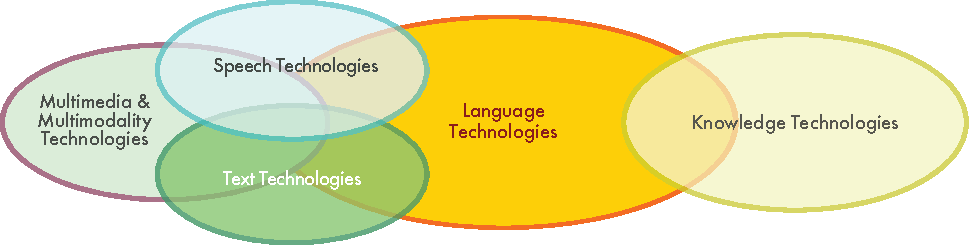
\includegraphics[width=\textwidth]{../_media/english/language_technologies}
  \caption{Language technologies}
  \refstepcounter{refs_en}
\label{fig:ltincontext_en}
  \colorrule{grey3}{\textwidth}{1.5pt}
\end{figure*}

When we communicate, we combine language with other modes of communication and information media – for example speaking can involve gestures and facial expressions. Digital texts link to pictures and sounds. Movies may contain language in spoken and written form. In other words, speech and text technologies overlap and interact with other multimodal communication and multimedia technologies.\\ 
In this section, we will discuss the main application areas of language technology, i.\,e., language checking, web search, speech interaction, and machine translation. These applications and basic technologies include

\begin{itemize}
\item spelling correction
\item authoring support
\item computer-assisted language learning
\item information retrieval 
\item information extraction
\item text summarisation
\item question answering
\item speech recognition 
\item speech synthesis 
\end{itemize}

Language technology is an established area of research with an extensive set of introductory literature.
%start Norwegian
The interested reader is referred to textbooks \cite{jurafsky-martin01, manning-schuetze1}, survey \cite{lt-survey1} and the website LT World (\url{http://www.lt-world.org}).
%end Norwegian

Before discussing the above application areas, we will briefly describe the architecture of a typical LT system.

\subsection{Application Architectures}

Software applications for language processing typically consist of several components that mirror different aspects of language. While such applications tend to be very complex, figure~\ref{fig:textprocessingarch_en} shows a highly simplified architecture of a typical text processing system. The first three modules handle the structure and meaning of the text input:

\begin{enumerate}
\item Pre-processing: cleans the data, analyses or removes formatting, detects the input languages, and so on.
\item Grammatical analysis: finds the verb, its objects, modifiers and other sentence elements; detects the sentence structure.
\item Semantic analysis: performs disambiguation (i.\,e., computes the appropriate meaning of words in a given context); resolves anaphora (i.\,e., which pronouns refer to which nouns in the sentence); represents the meaning of the sentence in a machine-readable way.
\end{enumerate}

After analysing the text, task-specific modules can perform other operations, such as automatic summarisation and database look-ups.

In the remainder of this section, we firstly introduce the core application areas for language technology, and follow this with a brief overview of the state of LT research and education today, and a description of past and present research programmes. Finally, we present an expert estimate of core LT tools and resources for Norwegian in terms of various dimensions such as availability, maturity and quality. The general situation of LT for the Norwegian language is summarised in figure~\ref{fig:lrlttable_en} (p.~\pageref{fig:lrlttable_en}) at the end of this chapter. This table lists all tools and resources that are boldfaced in the text. LT support for Norwegian is also compared to other languages that are part of this series.

\begin{figure*}[htb]
  \colorrule{grey3}{\textwidth}{1.5pt}
  \center
  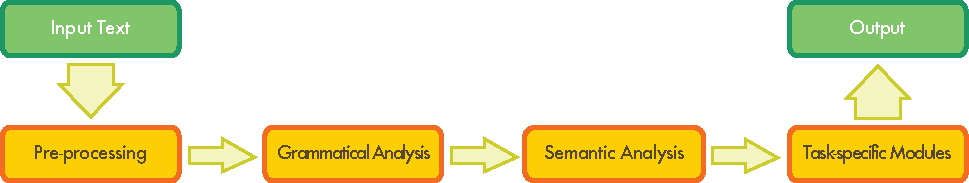
\includegraphics[width=\textwidth]{../_media/english/text_processing_app_architecture}
  \caption{A typical text processing architecture}
  \refstepcounter{refs_en}
\label{fig:textprocessingarch_en}
  \colorrule{grey3}{\textwidth}{1.5pt}
\end{figure*}

\subsection{Core Application Areas}

In this section, we focus on the most important LT tools and resources, and provide an overview of LT activities in 
%start Norwegian
Norway. 
%end Norwegian

\subsubsection{Language Checking}

Anyone who has used a word processor such as Microsoft Word knows that it has a spell checker that highlights spelling mistakes and proposes corrections. The first spelling correction programs compared a list of extracted words against a dictionary of correctly spelled words. Today these programs are far more sophisticated. Using language-dependent algorithms for \textbf{grammatical analysis}, they detect errors related to morphology (e.\,g., plural formation) as well as syntax–related errors, such as a missing verb or a conflict of verb-subject agreement (e.\,g., \textit{she *write a letter}). However, most spell checkers will not find any errors in the following text, because all the words are correctly \textit{spelt} even though some word choices are in fact wrong \cite{zar1}:

\begin{quote}
  I have a spelling checker,\\
  It came with my PC.\\
  It plane lee marks four my revue\\
  Miss steaks aye can knot sea.
\end{quote}

%start Norwegian
Handling these kinds of errors usually requires an analysis of the context, for example to decide if a Norwegian word should be spelled with one or with a double consonant in Norwegian, as in \textit{vil} (will, would like to) vs. \textit{vill} (wild).

This type of analysis either needs to draw on language-specific \textbf{grammars}, laboriously coded into the software by experts, or on a statistical language model. The latter calculates the probability of a particular word as it occurs in a specific position. For example, \textit{eg vil ha} (I would like to have) is a much more probable word sequence than \textit{eg vill ha} (I wild have). A statistical language model can be automatically created by using a large amount of (correct) language data, a \textbf{text corpus}.

Implementations of these two approaches have been developed around data from English. Neither approach can transfer easily to Norwegian with its different word order, compound building and richer inflection for certain word classes than in English, and studies for Norwegian are therefore needed. Furthermore, due to the particularity that Norwegian has two official written norms, one of which is lesser used, the need for good proofing tools for each written norm is significant. 
%end Norwegian

\begin{figure*}[htb]
  \colorrule{grey3}{\textwidth}{1.5pt}
  \center
  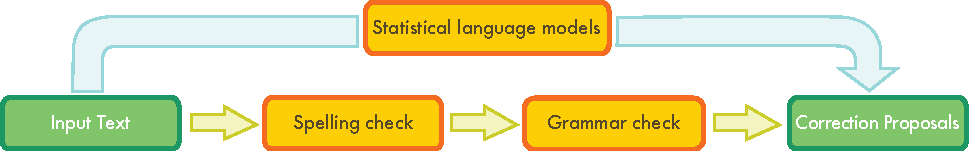
\includegraphics[width=\textwidth]{../_media/english/language_checking}
  \caption{Language checking (top: statistical; bottom: rule-based)}
  \refstepcounter{refs_en}
\label{fig:langcheckingaarch_en}
  \colorrule{grey3}{\textwidth}{1.5pt}
\end{figure*}

Language checking is not limited to word processors; it is also used in “authoring support systems”, i.\,e., software environments in which manuals and other types of technical documentation for complex IT, healthcare, engineering and other products, are written. To offset customer complaints about incorrect use and damage claims resulting from poorly understood instructions, companies are increasingly focusing on the quality of technical documentation while targeting the international market (via translation or localisation) at the same time. Advances in natural language processing have led to the development of authoring support software, which helps the writer of technical documentation to use vocabulary and sentence structures that are consistent with industry rules and (corporate) terminology restrictions.

\boxtext{Language checking is not limited to word processors but also applies to authoring systems.}

%start Norwegian
Adequate spell checkers would provide an important tool to alleviate the writing process for individuals with writing difficulties, be it dyslectics or second language learners, since a context sensitive analysis may enable fewer and more relevant spelling suggestions: many choices demand a high level of reading ability and linguistic awareness.

Some Norwegian companies and language service providers develop products in the area of language checking. 
On the research side, basic LT resources that may be of use for Language Checking (lexicons, word lists, text corpora, compound analysers) are developed mainly at the University of Oslo, the University of Bergen and Uni Research in Bergen. 

The most widely used proofing tool for Norwegian, the one found in the Microsoft Office suite, is made by the Finnish company Lingsoft, while parts of its grammar checker for Bokmål were developed by researchers at the University of Oslo. 
Spell checking for Bokmål and Nynorsk using open source technologies such as \textit{Hunspell} are also available.
Another Norwegian commercial actor is Tansa, which specialises in text proofing tools that are tuned to the specific needs and vocabularies of individual larger enterprises. 
Covering several languages in addition to Norwegian Bokmål and Nynorsk
(e.\,g., English, German, Spanish and French), their customers range from the Norwegian Broadcasting Corporation NRK to the Financial Times. 
Nynodata AS offers a writing aid tool from Bokmål to Nynorsk which translates and also ensures that the resulting word inflections adheres to the user’s chosen writing norm.

Three companies specifically target writing aid tools for dyslectics. 
Two of them, Lingit and Include, include a spell checker component as well as other reading and writing aid tools (word prediction, text-to-speech components), while MikroVerkstedet includes word completion and word prediction components.

On the face of it, the situation for Norwegian proofing tools may seem quite encouraging. 
But at the same time, several of the initiatives are quite fragile. 
For instance, Norwegian spell checking based on open source technologies (\textit{aspell, Hunspell}) is maintained by three individuals who use their spare time to do so. 
One may say that one of the major competitors to Microsoft software on the Norwegian market hinges on the personal initiatives of a few dedicated individuals rather than a systematic effort towards the development of open source modules. Moreover, a significant challenge for most Norwegian proofing tools is to \textit{improve} the existing basic resources by developing more advanced Language Technology tools. 

Finally, language specific tools for automatic translation or translation support of Norwegian are missing. Translation memory tools such as Trados exist, but they do not contain language specific adjustment for Norwegian beyond basic spell checking.

Besides spell checkers and authoring support, language checking is also important in the field of computer-assisted language learning. Language checking applications also automatically correct search engine queries, as found in Google's \textit{Did you mean…} suggestions.
%end Norwegian

\subsubsection{Web Search}

\begin{figure*}[htb]
  \colorrule{grey3}{\textwidth}{1.5pt}
  \center
  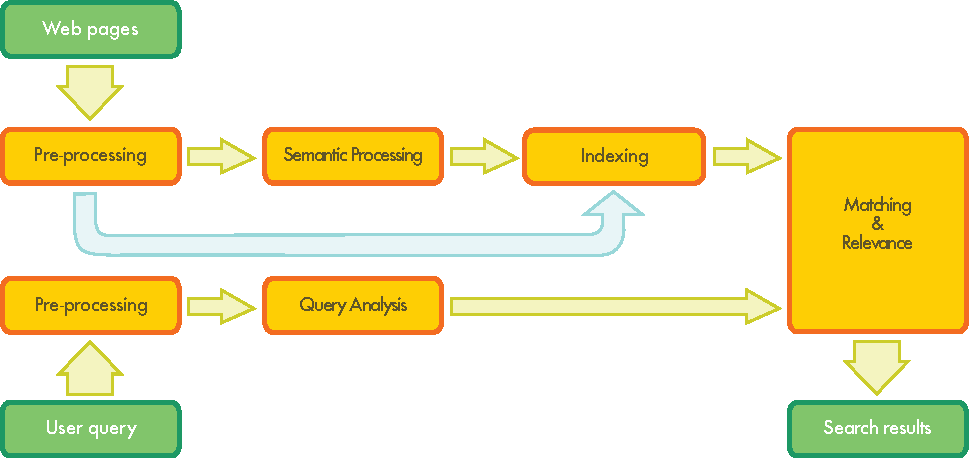
\includegraphics[width=\textwidth]{../_media/english/web_search_architecture}
  \caption{Web search}
  \refstepcounter{refs_en}
\label{fig:websearcharch_en}
  \colorrule{grey3}{\textwidth}{1.5pt}
 \end{figure*}

Searching the Web, intranets or digital libraries is probably the most widely used yet largely underdeveloped language technology application today. The Google search engine, which started in 1998, now handles about 80\% of all search queries \cite{spi1}. 
The Google search interface and results page display has not significantly changed since the first version. However, in the current version, Google offers spelling correction for misspelled words and incorporates basic semantic search capabilities that can improve search accuracy by analysing the meaning of terms in a search query context \cite{pc1}. The Google success story shows that a large volume of data and efficient indexing techniques can deliver satisfactory results using a statistical approach to language processing. 

For more sophisticated information requests, it is essential to integrate deeper linguistic knowledge to facilitate text interpretation. Experiments using \textbf{lexical resources} such as machine-readable thesauri or ontologies
%start Norwegian
(a Norwegian wordnet is expected by the end of 2012)
%end Norwegian
have demonstrated improvements in finding pages using synonyms of the original search terms, such as
\textit{atomkraft} (atomic energy), \textit{kjerneenergi} (atomic power) and \textit{nukleærenergi} (nuclear energy),
or even more loosely related terms.

\boxtext{The next generation of search engines\\ will have to include much more sophisticated language technology.}

The next generation of search engines will have to include much more sophisticated language technology, especially to deal with search queries consisting of a question or other sentence type rather than a list of keywords. For the query \textit{Give me a list of all companies that were taken over by other companies in the last five years}, a syntactic as well as \textbf{semantic analysis} is required. The system also needs to provide an index to quickly retrieve relevant documents. A satisfactory answer will require syntactic parsing to analyse the grammatical structure of the sentence and determine that the user wants companies that have been acquired, rather than companies that have acquired other companies. For the expression \textit{last five years}, the system needs to determine the relevant range of years, taking into account the present year. The query then needs to be matched against a huge amount of unstructured data to find the pieces of information that are relevant to the user’s request. This process is called information retrieval, and involves searching and ranking relevant documents. To generate a list of companies, the system also needs to recognise a particular string of words in a document represents a company name, using a process called named entity recognition.

A more demanding challenge is matching a query in one language with documents in another language. Cross-lingual information retrieval involves automatically translating the query into all possible source languages and then translating the results back into the user's target language.

Now that data is increasingly found in non-textual formats, there is a need for services that deliver multimedia information retrieval by searching images, audio files and video data. In the case of audio and video files, a speech recognition module must convert the speech content into text (or into a phonetic representation) that can then be matched against a user query.

%start Norwegian
In Norway, Opera Software developed the first Norwegian web browser and Internet suite.
Opera began in 1994 as a research project within Norway’s largest telecom company, Telenor. 
Within a year, it demerged into an independent development company named Opera Software ASA.
A few companies develop or apply search solutions (CognIT, Comperio, TextUrgy, Abtrox and Infofinder). 
FAST developed a search engine, which was then bought by Microsoft, and which is now being traded by Comperio. 
The development focus for these companies lies on providing add-ons and advanced search engines by exploiting topic-relevant semantics. 
Thus, one may say that the IT industry in Norway already has quite a good foundation as regards web search and information retrieval; the main need reported from the companies is that of reliable LRT components.
%end Norwegian

\subsubsection{Speech Interaction}

Speech interaction is one of many application areas that depend on speech technology, i.\,e., technologies for processing spoken language. Speech interaction technology is used to create interfaces that enable users to interact in spoken language instead of using a graphical display, keyboard and mouse.  Today, these voice user interfaces (VUI) are used for partially or fully automated telephone services provided by companies to customers, employees or partners. Business domains that rely heavily on VUIs include banking, supply chain, public transportation, and telecommunications. Other uses of speech interaction technology include interfaces to car navigation systems and the use of spoken language as an alternative to the graphical or touchscreen interfaces in smartphones. 
Speech interaction technology comprises four technologies: 

\begin{figure*}[htb]
  \colorrule{grey3}{\textwidth}{1.5pt}
  \center
  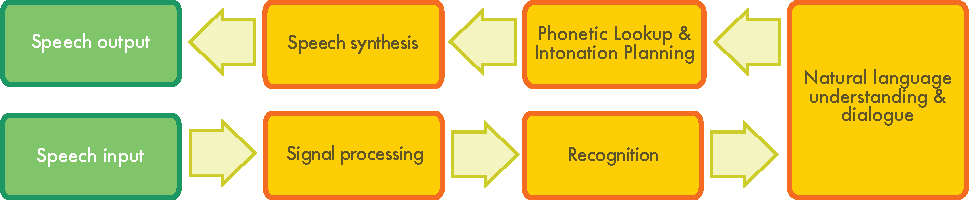
\includegraphics[width=\textwidth]{../_media/english/simple_speech-based_dialogue_architecture}
  \caption{Speech-based dialogue system}
  \refstepcounter{refs_en}
\label{fig:dialoguearch_en}
  \colorrule{grey3}{\textwidth}{1.5pt}
\end{figure*}

\begin{enumerate}
\item Automatic \textbf{speech recognition} (ASR) determines which words are actually spoken in a given sequence of sounds uttered by a user.  
\item Natural language understanding analyses the syntactic structure of a user’s utterance and interprets it according to the system in question.
\item Dialogue management determines which action to take given the user input and system functionality.   
\item \textbf{Speech synthesis} (text-to-speech or TTS) transforms the system’s reply into sounds for the user.
\end{enumerate}

One of the major challenges of ASR systems is to accurately recognise the words a user utters. This means restricting the range of possible user utterances to a limited set of keywords, or manually creating language models that cover a large range of natural language utterances. Using machine learning techniques, language models can also be generated automatically from \textbf{speech corpora}, i.\,e., large collections of speech audio files and text transcriptions. Restricting utterances usually forces people to use the voice user interface in a rigid way and can damage user acceptance; but the creation, tuning and maintenance of rich language models will significantly increase costs. VUIs that employ language models and initially allow a user to express their intent more flexibly -- prompted by a \textit{How may I help you?} greeting -- tend to be automated and are better accepted by users.

%\boxtext{Speech interaction is the basis for creating interfaces that allow a user to interact with spoken language instead of a graphical display, keyboard and mouse.}
\boxtext{Speech interaction is the basis for interfaces that allow a user to interact with spoken language.}

Companies tend to use utterances pre-recorded by professional speakers for generating the output of the voice user interface. For static utterances where the wording does not depend on particular contexts of use or personal user data, this can deliver a rich user experience. But more dynamic content in an utterance may suffer from unnatural intonation because different parts of audio files have simply been strung together. Through optimisation, today’s TTS systems are getting better at producing natural-sounding dynamic utterances.

Interfaces in speech interaction have been considerably standardised during the last decade in terms of their various technological components. There has also been strong market consolidation in speech recognition and speech synthesis. The national markets in the G20 countries (economically resilient countries with high populations) have been dominated by just five global players, with Nuance (USA) and Loquendo (Italy) being the most prominent players in Europe. In 2011, Nuance announced the acquisition of Loquendo, which represents a further step in market consolidation.

%start Norwegian
In the Norwegian TTS market, thirteen Norwegian voices of varying quality are available, some of which have been developed by the above mentioned European players. 
Three voices have been developed by the Norwegian company Lingit, which targets users groups with reading and writing impairments. 
Another voice was developed by the Norwegian Library of Talking Books and Braille in cooperation with their sister library in Sweden. 
There is also an active research community at the Norwegian University of Science and Technology in Trondheim. 

\boxtext{Language resources for speech synthesis are abundant for English but only to a lesser extent for Norwegian.}

The quality of speech synthesis depends heavily on available resources (in particular text corpora tagged for part of speech, tokenisers and pronunciation lexicons) and language specific research on for instance prosodic features for the language in question. 
Such resources are abundant for English but only to a lesser extent for Norwegian, even if Norwegian is especially challenging due to the wide variety of possible spelling variants and the range of dialects; moreover the tonal accents in most Norwegian dialects and the lack of a one-to-one relation between sounds and letters pose challenges.

Regarding dialogue management technology and know-how, the market is rather dominated by national, smaller enterprises. 
MediaLT has developed a general speech recognition engine used for dialogue management for the visually impaired. 
Regarding speech-to-text, Max Manus has integrated and localised Philips’ SpeechMagic for Norwegian hospitals. 
This system is relatively successful, but it is limited to a relatively closed domain (with a closed vocabulary). 
Recently Dragon Dictation, a voice recognition application for mobile telephones, was launched for Norwegian. 
This application is the first \textit{general} dictation system for Norwegian; however, the Norwegian version of Dragon Dictation seems to misinterpret conspicuously more than the English counterpart.
Within the domain of speech interaction, a genuine market for the linguistic core technologies for syntactic and semantic analysis does not exist yet.
%end Norwegian

Looking ahead, there will be significant changes, due to the spread of smartphones as a new platform for managing customer relationships, in addition to fixed telephones, the Internet and e-mail. This will also affect how speech interaction technology is used. In the long term, there will be fewer telephone-based VUIs, and spoken language apps will play a far more central role as a user-friendly input for smartphones. This will be largely driven by stepwise improvements in the accuracy of speaker-independent speech recognition via the speech dictation services already offered as centralised services to smartphone users.

\subsubsection{Machine Translation}

\begin{figure*}[htb]
  \colorrule{grey3}{\textwidth}{1.5pt}
  \center
  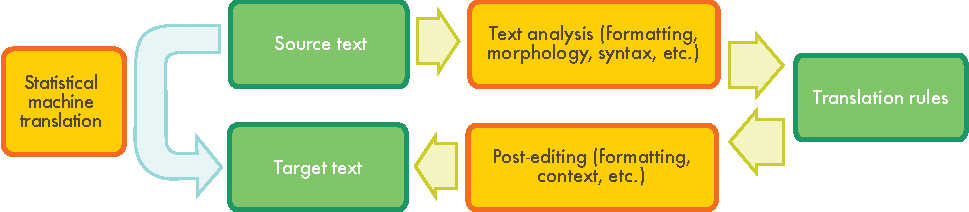
\includegraphics[width=\textwidth]{../_media/english/machine_translation}
  \caption{Machine translation (left: statistical; right: rule-based)}
  \refstepcounter{refs_en}
\label{fig:mtarch_en}
  \colorrule{grey3}{\textwidth}{1.5pt}
\end{figure*}

The idea of using digital computers to translate natural languages can be traced back to 1946 and was followed by substantial funding for research during the 1950s and again in the 1980s. 
Yet \textbf{machine translation} (MT) still cannot deliver on its initial promise of providing across-the-board automated translation.  

The most basic approach to machine translation is the automatic replacement of the words in a text written in one natural language with the equivalent words of another language. This can be useful in subject domains that have a very restricted, formulaic language such as weather reports.
However, in order to produce a good translation of less restricted texts, larger text units (phrases, sentences, or even whole passages) need to be matched to their closest counterparts in the target language. 

\boxtext{The major difficulty for Machine Translation is that human language is ambiguous.}

%start Norwegian
The major difficulty is that human language is ambiguous. Ambiguity creates challenges on multiple levels, such as word sense disambiguation at the lexical level or syntactic ambiguities at the sentence level. 
A likely idiomatic translation of the Norwegian sentence \textit{Plutseleg rauk slangen} in English could be \textit{Suddenly the hose snapped.}
However, a simple word-by-word translation of this sentence might yield \textit{Suddenly smoked the snake.}
This is because the verb form \textit{rauk} (past tense of \textit{ryke}) is ambiguous between `snap' and `smoke' whereas \textit{slange} is ambiguous between `hose' and `snake'; note also that a simple word-by-word translation would not get the difference in word order between Norwegian and English right.

In addition to lexical ambiguities and word order differences, another challenge is syntactic ambiguities. 
In Norwegian we may topicalise objects, but this possibility is much more restricted in English. 
The Norwegian sentence \textit{epla spiste mannen} has two possible interpretations: either \textit{epla} (the apples) is analysed as the subject of the sentence (the apples ate the man) or as a topicalised object (the apples were eaten by the man). 
Since this ambiguity does not exist in English, a machine translation system must first identify the correct syntactic interpretation in order to find the correct translation. 

Another MT challenge for Norwegian is compounding. 
An efficient translation system must thus be able to discover newly coined compounds, resolve them, and, if needed, create new compounds in the target language. 
%end Norwegian

For translations between closely related languages, a translation using direct substitution may be feasible for many sentences. However, rule-based (or linguistic knowledge-driven) systems often analyse the input text and create an intermediary symbolic representation from which the target language text can be generated. The success of these methods is highly dependent on the availability of extensive lexicons with morphological, syntactic, and semantic information, and large sets of grammar rules carefully designed by skilled linguists. This is a very long and therefore costly process.

In the late 1980s when computational power increased and became cheaper, interest in statistical models for machine translation began to grow. Statistical models are derived from analysing bilingual text corpora, \textbf{parallel corpora}, such as the Europarl parallel corpus, which contains the proceedings of the European Parliament in 21 European languages
%start Norwegian
(Norwegian not being one of them).
%end Norwegian
Given enough data, statistical MT works well enough to derive an approximate meaning of a foreign language text by processing parallel versions and finding plausible patterns of words. Unlike knowledge-driven systems, however, statistical (or data-driven) MT systems often generate ungrammatical output. Data-driven MT is advantageous because less human effort is required, and it can also cover special particularities of the language (e.\,g., idiomatic expressions) that are often ignored in knowledge-driven systems. 

The strengths and weaknesses of knowledge-driven and data-driven machine translation tend to be complementary, so that nowadays researchers focus on hybrid approaches that combine both methodologies. One such approach uses both knowledge-driven and data-driven systems, together with a selection module that decides on the best output for each sentence. However, results for sentences longer than, say, 12 words, will often be far from perfect. A more effective solution is to combine the best parts of each sentence from multiple outputs; this can be fairly complex, as corresponding parts of multiple alternatives are not always obvious and need to be aligned. 

\boxtext{Although the need for Machine Translation for Norwegian is apparent, the development of such software for Norwegian is not extensive.}

Two systems address the fact that Norwegian has two written norms, creating a need for efficient translations between the written norms. 
The small enterprise Nynodata offers tools for translation, correction and text search for Bokmål and Nynorsk. 
The open-source initiative Apertium also offers automated translation between the two written norms, implemented by a student at the University of Bergen. 

Google Translate has a Norwegian module to translate between English and Norwegian, and via English it is possible to translate between Norwegian and any language pair containing English. 
GramTrans is an MT platform developed in cooperation between the Danish GrammarSoft ApS and the Norwegian company Kaldera Språkteknologi AS. 
The translation engine offers free web-based translation for the Scandinavian languages and also between Norwegian and English, based on a robust grammatical analysis, a transfer component for lexicon and grammar and a generation component. 
The company Clue Norge, which specialises in electronic dictionaries for enterprises, developed a system (Textran) for machine translation from English to Norwegian about ten years ago. 
The system still exists but was not further developed because perfect translations are hard to obtain whereas the user groups were not ready to pay for a less than perfect system.

Although significant research in this technology exists in national and international contexts, data-driven and hybrid systems have so far been less successful in business applications than in the research lab. 
In Norway, the main research expertise in this field is found at the University of Oslo and the University of Bergen.

\boxtext{There seems to be an underuse of language technology resources in the Norwegian Language Service Industry}

The use of machine translation can significantly increase productivity provided the system is intelligently adapted to user-specific terminology and integrated into a workflow. 
In general, there seems to be an underuse of language technology resources in the Norwegian Language Service Industry. 
This sector can be divided into two groups: on the one hand there are freelance translators and translation agencies catering to individual clients, commercial actors and the public sector, and on the other hand there are translators affiliated with \textit{Oversetterforeningen} (Organisation of translators of literary texts) and \textit{Norsk faglitterær forfatter- og oversetterforening} (Organisation of translators of scientific and academic texts). In the latter group, the use of language technology is limited. 
The former group uses Trados, which is the dominant machine translation tool for professional translators. 
However, Trados has no Norwegian module but is based on Hunspell, an open source spell checker and morphological analyser originally developed for Hungarian which is not optimal for Norwegian. 
Although it is a functional and open solution, it still needs further development to be an optimal resource for the Norwegian Language Service industry and there is a particular need for improvement of the analysis of Norwegian compounds. 

In addition, professional translators use term bases (UD, IATE) and to some extent collaborate with the University Sector in developing term base resources. 
The apparent underuse of language technology resources in the Language Service Industry is caused in part by the lack of adequate resources for Norwegian, but also by a lacking contact between the Language Service Industry and the research community. 
As a consequence, knowledge of the full spectrum of language technology is often too limited, and it is difficult for commercial actors to evaluate the quality of a resource. 
%end Norwegian

There is still a huge potential for improving the quality of MT systems. The challenges involve adapting language resources to a given subject domain or user area, and integrating the technology into workflows that already have term bases and translation memories. Another problem is that most of the current systems are English-centred and only support a few languages from and into German. This leads to friction in the translation workflow and forces MT users to learn different lexicon coding tools for different systems.

Evaluation campaigns help to compare the quality of MT systems, the different approaches and the status of the systems for different language pairs.
%start Norwegian
Figure~\ref{fig:euromatrix_de} (p.~\pageref{fig:euromatrix_de}), prepared during the EuroMatrix+ project, shows the pair-wise performances obtained for 22 of the 23 EU languages (Irish was not compared). The results are ranked according to a BLEU score, which indicates higher scores for better translations \cite{bleu1}. A human translator would normally achieve around 80 points. The best results (in green and blue) were achieved by languages that benefit from a considerable research effort in coordinated programmes and many parallel corpora (e.\,g., English, French, Dutch, Spanish and German). Poorer results are shown in red. These either lack such development efforts or are structurally very different from other languages (e.\,g., Hungarian, Maltese, Finnish). Norwegian was not included in this project.
%end Norwegian

\subsection{Other Application Areas}

Building language technology applications involves a range of subtasks that do not always surface at the level of interaction with the user, but they provide significant service functionalities “behind the scenes” of the system in question. They all form important research issues that have now evolved into individual sub-disciplines of computational linguistics.  Question answering, for example, is an active area of research for which annotated corpora have been built and scientific competitions have been initiated. The concept of question answering goes beyond keyword-based searches (in which the search engine responds by delivering a collection of potentially relevant documents) and enables users to ask a concrete question to which the system provides a single answer. For example:

\begin{itemize}
\item[] \textit{Question: How old was Neil Armstrong when he stepped on the moon?}
\item[] \textit{Answer: 38.}
\end{itemize}

While question answering is obviously related to the core area of web search, it is nowadays an umbrella term for such research issues as which different types of questions exist, and how they should be handled; how a set of documents that potentially contain the answer can be analysed and compared (do they provide conflicting answers?); and how specific information (the answer) can be reliably extracted from a document without ignoring the context. 

Question answering is in turn related to information extraction (IE), an area that was extremely popular and influential when computational linguistics took a statistical turn in the early 1990s. IE aims to identify specific pieces of information in specific classes of documents, such as the key players in company takeovers as reported in newspaper stories. Another common scenario that has been studied is reports on terrorist incidents. The task here consists of mapping appropriate parts of the text to a template that specifies the perpetrator, target, time, location and results of the incident. Domain-specific template-filling is the central characteristic of IE, which makes it another example of a “behind the scenes” technology that forms a well-demarcated research area, which in practice needs to be embedded into a suitable application environment. 

%\boxtext{Language technology applications often provide significant service functionalities behind the scenes of larger software systems.}

Text summarisation and \textbf{text generation} are two borderline areas that can act either as standalone applications or play a supporting role. Summarisation attempts to give the essentials of a long text in a short form, and is one of the features available in Microsoft Word. It mostly uses a statistical approach to identify the “important” words in a text (i.\,e., words that occur very frequently in the text in question but less frequently in general language use) and determine which sentences contain the most of these “important” words. These sentences are then extracted and put together to create the summary. In this very common commercial scenario, summarisation is simply a form of sentence extraction, and the text is reduced to a subset of its sentences. An alternative approach, for which some research has been carried out, is to generate brand new sentences that do not exist in the source text. 

%start Norwegian
\boxtext{For Norwegian, research in most text technologies is much less developed than for English.}

This requires a deeper understanding of the text, which means that so far this approach is far less robust. On the whole, a text generator is rarely used as a stand-alone application but is embedded into a larger software environment, such as a clinical information system that collects, stores and processes patient data. Creating reports is just one of many applications for text summarisation.

Question answering, information extraction, and summarisation have been the focus of numerous open competitions in the USA since the 1990s, primarily organised by the government-sponsored organisations DARPA and NIST. 
These competitions have significantly improved the start-of-the-art, but their focus has mostly been on the English language. 
As a result, there are hardly any annotated corpora or other special resources needed to perform these tasks in Norwegian. 
When summarisation systems use purely statistical methods, they are largely language-independent and a number of research prototypes are available. 
For text generation, reusable components have traditionally been limited to surface realisation modules (generation grammars) and most of the available software is for the English language.
%end Norwegian

\subsection{Educational Programmes}

Language technology is a very interdisciplinary field that involves the combined expertise of linguists, computer scientists, mathematicians, philosophers, psycholinguists, and neuroscientists among others. 
%start Norwegian
As a result, it has not acquired a clear, independent existence in the Norwegian higher education system. 

In Norway, scientific expertise is present in small research groups at the universities of Oslo, Bergen, and Tromsø, the Norwegian University of Science and Technology, the Norwegian School of Economics and the research companies Uni Research and Sintef) that cooperate on a project basis. 
No universities have established separate departments or centres of Computational Linguistics or Language Technology. 
%GIL: fjernet fra følgende originalsetning at datalingvistikkundervisning foregår BÅDE ved lingvistikk/UiO og infirmatikk/UiO: A limited number of relevant courses are offered by departments of Computer Science (University of Oslo and Norwegian University of Science and Technology) and Linguistics (Universities of Bergen, Oslo and Tromsø). 
A limited number of relevant courses are offered by departments of Computer Science (University of Oslo and Norwegian University of Science and Technology) and Linguistics (Universities of Bergen and Tromsø). 
Research and teaching in speech processing is only represented at the Norwegian University of Science and Technology. 

\boxtext{Language technology has not acquired a clear, independent existence in the Norwegian higher education system.}

Although it is hard to quantify such a claim, the field of Computational Linguistics, and the options to study it, do not appear to be very well-known in Norway. 
Indeed, a crux of the KUNSTI programme was to strengthen basic research and the competence within language technology disciplines. %\footnote{http://www.forskningsradet.no/servlet/Satellite?c=Page\&pagename=kunsti\%2FHovedsidemal\&cid=1232959399366}. 
%KUNSTI \footnote{http://www.forskningsradet.no/servlet/Satellite?c=Page\&cid=1232959399409\&pagename=kunsti\%2FHovedsidemal}
This programme enabled several master's and PhD theses to be completed in relation to the wide variety of research projects. 
One may therefore say that this programme was instrumental in stimulating a framework to foster new researchers and a wider competence in LRT for Norwegian.

The University of Bergen coordinates CLARA, a Marie Curie Initial Training Network aimed at offering researcher training in LRT at nine European facilities.

\subsection{National Projects and Initiatives}

Since the Norwegian language industry is relatively small by international standards, national and local academic initiatives have been important for the development of Norwegian LRT, also for the benefit of private companies.
Most Norwegian companies in need of LRT express their desire to take advantage of resources, knowledge and expertise in academia, because their own main expertise usually does not lie in LRT.

The Research Council of Norway has supported one language technology research programme, namely KUNSTI (Kunnskapsutvikling for norsk språkteknologi).
It was in part inspired by larger projects in other countries (e.\,g.,
the German project Verbmobil) and aimed to increase competence in language technology through basic research. 
KUNSTI aimed for R\&D to make spoken and written Norwegian in various forms (and to some extent Saami) accessible for computer processing. 
Twenty research projects of varying sizes were completed under the programme, the largest two being in MT and speech processing. Building a variety of language technology applications presupposes basic resources, such as word lists, text corpora and speech corpora. 
These are just as costly and time-consuming to develop for smaller languages as for larger languages; since Norwegian has two official written norms, the costs are even higher. 
Therefore, Norwegian is not very attractive from a commercial point of view. 

\boxtext{\textit{Språkbanken} is one of the most important language policy investments\\ in Norway in recent times.}

It is for this reason that it was such an important achievement to establish the \textit{Language Technology Resource Collection for Norwegian -- Språkbanken} in 2010. % after two decades of joint efforts between the Norwegian Language Council, the Research Council, commercial companies and the Norwegian research institutions. 
Språkbanken at the National Library is to function as an infrastructure for making Norwegian LRT available for research and commercial use, thus hopefully reducing the threshold for developing Norwegian LRT products. 

The situation thus far has been that whereas private companies compile various in-house resources and tools,
substantial resources and tools (e.\,g., lexicons, taggers and named-entity recognisers) are developed at research institutions and subsequently sometimes purchased in some form by private companies. 
Indeed, the majority of tools and resources listed in the Table of Tools and Resources at the end of this report are developed at the research institutions. 
For instance, the University of Oslo has developed the speech corpora NoTa-Oslo (Norsk Talespråkskorpus, the Oslo part) and Nordic Dialect Corpus, Norsk Ordbank has been developed by the University of Oslo in cooperation with the Norwegian Language Council, the Oslo-Bergen tagger has been made by the University of Oslo and Uni Research in Bergen, the Norwegian Newspaper Corpus has been developed by Uni Research and the Norwegian School of Economics and the INESS treebanking infrastructure is currently being built at the University of Bergen.

In the work programme of KUNSTI, the development of basic language and speech data was not catered for. 
It was therefore felt that the projects under this programme were hampered by a lack of basic language resources. 
With Språkbanken now established, and with new researchers and revitalised competence, it is felt by many that the time may be ripe to consider a new LRT effort which may get a more application-oriented focus than its predecessor. 

Sizeable LRT building projects (e.\,g., the INESS, NoTa-Oslo, Norsk
aviskorpus, WeSearch-Language technology for the web and SIRKUS) after KUNSTI have been financed through infrastructure programmes (AVIT) or general ICT programmes from the Research Council such as VERDIKT. 
%As a part of building basic Norwegian LRT, Språkbanken signed a contract with Kaldera språkteknologi AS in 2011 to create wordnets for Norwegian. % Bokmål and Nynorsk. %\footnote{http://www.nb.no/spraakbanken/english/projects}. 
Public funding for LT projects in Norway and in Europe is still relatively low, however, when compared to the amount of money the USA spends on language translation and multilingual information access \cite{laz1}.

As we have seen, previous programmes have led to the development of a number of LT tools and resources for the Norwegian language. In the following section, the current state of LT support for Norwegian is summarised.
  
\subsection{Availability of Tools and Resources}

Figure~\ref{fig:lrlttable_en} provides a rating for language technology support for Norwegian. This rating of existing tools and resources was generated by leading experts in the field who provided estimates based on a scale from 0 (very low) to 6 (very high) using seven criteria.

%the following table needs numbers for Norwegian
\begin{figure*}[htb]
\centering
%\begin{tabular}{>{\columncolor{orange1}}p{.33\linewidth}ccccccc} % ORIGINAL
\begin{tabular}{>{\columncolor{orange1}}p{.33\linewidth}@{\hspace*{6mm}}c@{\hspace*{6mm}}c@{\hspace*{6mm}}c@{\hspace*{6mm}}c@{\hspace*{6mm}}c@{\hspace*{6mm}}c@{\hspace*{6mm}}c}
\rowcolor{orange1}
 \cellcolor{white}&\begin{sideways}\makecell[l]{Quantity}\end{sideways}
&\begin{sideways}\makecell[l]{\makecell[l]{Availability} }\end{sideways} &\begin{sideways}\makecell[l]{Quality}\end{sideways}
&\begin{sideways}\makecell[l]{Coverage}\end{sideways} &\begin{sideways}\makecell[l]{Maturity}\end{sideways} &\begin{sideways}\makecell[l]{Sustainability~~~}\end{sideways} &\begin{sideways}\makecell[l]{Adaptability}\end{sideways} \\ \addlinespace
\multicolumn{8}{>{\columncolor{orange2}}l}{Language Technology: Tools, Technologies and Applications} \\ \addlinespace
Speech Recognition &4&2&2&1&2&3&3 \\ \addlinespace
Speech Synthesis &3&2&3&2&3&3&3\\ \addlinespace
Grammatical analysis &4&4,5&4&4&4,5&4,5&5\\ \addlinespace 
Semantic analysis &2&2&3,3&3&3,7&3,3&3,7\\ \addlinespace
Text generation &1&4&4&3&5&4&5\\ \addlinespace
Machine translation &4&4&2&2&3&5&3\\ \addlinespace
\multicolumn{8}{>{\columncolor{orange2}}l}{Language Resources: Resources, Data and Knowledge Bases} \\ \addlinespace
Text corpora &4,5&3,5&3,5&3&4&4,5&4\\ \addlinespace
Speech corpora &5&4&3&5&4&5&5\\ \addlinespace
Parallel corpora &5&3&2&2&4&3&3\\ \addlinespace
Lexical resources &2,5&2&2&2&2&2&2,5\\ \addlinespace
Grammars &2&4&5&3&4&5&3\\
\end{tabular}
\caption{State of language technology support for Norwegian}
\refstepcounter{refs_en}
\label{fig:lrlttable_en}
\end{figure*}

The key results for Norwegian language technology can be summed up as follows:

\begin{itemize}
\item Norwegian stands reasonably well with respect to the most basic language technology tools and resources, such as tokenisers, PoS taggers, morphological analysers, reference corpora, and speech corpora. 
There are also many speech synthesis (TTS) products for Norwegian with a general applicability and an acceptable quality, although most of them are developed by commercial actors and are thus restricted in terms of availability. Lexicons covering general language are well-represented but there are major gaps in the coverage of terminologies representing specialised domains.
\item Individual products with limited functionality exist in subfields such as speech recognition, machine translation, text semantics and a few others. 
Some of these areas are covered for Norwegian by commercial actors and are thus restricted in terms of availability.
\item Some tools and resources are virtually non-existing; furthermore some resources are developed for commercial use and are not available. 
This typically applies to tools and resources for more advanced Norwegian language technology such as a advanced discourse processing, text generation and ontologies for representing world knowledge.
\item At present, many of the tools and resources lack standardisation, i.\,e., even if they exist, sustainability and adaptability are not necessarily catered for. 
Although the table suggests that basic LT tools and resources exist for Norwegian, they are in some cases fragmented and their sustainability is limited by restrictions on their use, incompatibilities and insufficient documentation. 
\end{itemize}

To conclude, today we have software with limited functionality available in a number of specific areas of Norwegian language research. 
Obviously, further research efforts are required to meet the current deficit in processing texts on a deeper semantic level and to address the lack of resources such as parallel corpora for machine translation.
%end Norwegian

\subsection{Cross-language comparison}


The current state of LT support varies considerably from one language community to another. In order to compare the situation between languages, this section will present an evaluation based on two sample application areas (machine translation and speech processing) and one underlying technology (text analysis), as well as basic resources needed for building LT applications. The languages were categorised using the following five-point scale: 

\begin{enumerate}
\item Excellent support
\item Good support
\item Moderate support
\item Fragmentary support
\item Weak or no support
\end{enumerate}

LT support was measured according to the following criteria:

\textbf{Speech Processing:} Quality of existing speech recognition technologies, quality of existing speech synthesis technologies, coverage of domains, number and size of existing speech corpora, amount and variety of available speech-based applications.

\textbf{Machine Translation:} Quality of existing MT technologies, number of language pairs covered, coverage of linguistic phenomena and domains, quality and size of existing parallel corpora, amount and variety of available MT applications.

\textbf{Text Analysis:} Quality and coverage of existing text analysis technologies (morphology, syntax, semantics), coverage of linguistic phenomena and domains, amount and variety of available applications, quality and size of existing (annotated) text corpora, quality and coverage of existing lexical resources (e.\,g., WordNet) and grammars.

\textbf{Resources:} Quality and size of existing text corpora, speech corpora and parallel corpora, quality and coverage of existing lexical resources and grammars.

%start Norwegian
Figures~\ref{fig:speech_cluster_en} to~\ref{fig:resources_cluster_en} show that LT resources and tools for Norwegian clearly do not yet reach the quality and coverage of comparable resources and tools for the English language, which is in the lead in almost all LT areas. 
Moreover, there are still many gaps even in English language resources with regard to high quality applications. 
The situation for Norwegian compares well with our neighbouring languages, although the figures fail to show mismatches between the situation for Bokmål on the one hand and Nynorsk on the other hand. 

\boxtext{Our study shows that LT resources and tools for Norwegian clearly do not yet reach the quality and coverage of comparable resources and tools for the English language, which is in the lead in almost all LT areas. }

For speech synthesis, several Norwegian-speaking voices are available in end-user applications, although many platforms do not offer free, adaptive and high quality Norwegian speech synthesis that could be used by developers. 
For speech recognition there is low support for Norwegian; there are no general speech recognisers with the possible exception of the recently launched mobile application Dragon Dictation, which could not be assessed in time for the present report.
There is one specialised recogniser for medical records with varying quality.

For machine translation between Norwegian Bokmål and Nynorsk, one bidirectional, freely available application and one unidirectional, commercial application exist. 
For machine translation from Norwegian to other languages there is one free resource and one commercial application available with varying quality and performance. 

Today’s text analysis components cover the linguistic phenomena of
Norwegian to a certain extent and form part of many applications
involving mostly shallow natural language processing, e.\,g., general spelling correction and writing aid tools for dyslectics. 

As far as resources are concerned, the previous section has already pointed to conspicuous gaps.
%end Norwegian
For building more sophisticated applications, such as machine translation, there is a clear need for resources and technologies that cover a wider range of linguistic aspects and enable a deep semantic analysis of the input text. By improving the quality and coverage of these basic resources and technologies, we shall be able to open up new opportunities for tackling a broader range of advanced application areas, including high-quality machine translation.

\subsection{Conclusions}

\emph{In this series of white papers, we have made an important effort by assessing the language technology support for 30 European languages, and by providing a high-level comparison across these languages. By identifying the gaps, needs and deficits, the European language technology community and its related stakeholders are now in a position to design a large scale research and development programme aimed at building a truly multilingual, technology-enabled communication across Europe.}

The results of this white paper series show that there is a dramatic difference in language technology support between the various European languages. While there are good quality software and resources available for some languages and application areas, other (usually smaller) languages have substantial gaps. Many languages lack basic technologies for text analysis and the essential resources. Others have basic tools and resources, but there is little chance of implementing semantic methods in the near future. Therefore a large-scale effort is needed to attain the ambitious goal of providing high-quality language technology support for all European languages, for example through high quality machine translation. 

%start Norwegian
In the case of the Norwegian language, we have seen that technologies that were developed and optimised for the English language do not easily transfer to Norwegian. 
It costs just as much to develop language resources for a small language as for a larger language. 
It is therefore important to continue the public support for R\&D for Norwegian LT, even more so since Norwegian has two written norms that must be catered for. 
The required level of investment has not been reached thus far. The Norwegian language technology industry dedicated to transforming research into products is currently fragmented and disorganised. The field is characterised by specialised SMEs that are not robust enough to address the internal and the global market with a sustained strategy. 

Specifically, the most urgent needs of Norwegian Language Technology are:
\begin{enumerate}
\item Improved licensing conditions and standardisation of existing basic tools and resources, in order to make them openly available to the research community and industry.
\item Creation of missing basic tools and resources, including multilingual tools with Norwegian as source or target language, in standard formats with open licenses.
\item Basic research on the higher levels of automatic linguistic analysis for Norwegian, and on the integration of statistical and rule-based LT, not least in order to aim for a closer interaction between speech and text technology.
\item Coordinated dissemination of research results to improve their visibility to potential users and to attract new scholars/students to the field.
\item Long term funding strategies for securing the development of LRT for both Norwegian written norms and for the minority languages.
\end{enumerate}

For a small language community such as Norwegian and a small research
environment, cooperation is vital, not only on the national level but
also internationally. Since 2000, Norwegian researchers and policy
makers have taken an active part in Nordic cooperation (e.\,g., the Nordic Language Technology Research Programme 2000–2004). It is also hoped that Norway’s participation in CLARIN and META-NORD will make set an example to develop, standardise and share several important LRT and thus contribute to the growth of Norwegian language technology in a context of European cooperation. This should be followed up by a better overall coordination with programmes in other EU countries and at the European Commission level.

%Our findings lead to the conclusion that the only way forward is to make a substantial effort to create language technology resources for German, as a means to drive forward research, innovation and development. The need for large amounts of data and the extreme complexity of language technology systems makes it vital to develop an infrastructure and a coherent research organisation to spur greater sharing and cooperation.

%Finally there is a lack of continuity in research and development funding. Short-term coordinated programmes tend to alternate with periods of sparse or zero funding. In addition, there is an overall lack of coordination with programmes in other EU countries and at the European Commission level.

The long term goal of META-NET is to enable the creation of high-quality language technology for all languages. This requires all stakeholders --- in politics, research, business, and society --- to unite their efforts. The resulting technology will help tear down existing barriers and build bridges between Europe’s languages, paving the way for political and economic unity through cultural diversity. 

\end{multicols}

\clearpage

\begin{figure*}[tb]
  \small
  \centering
  \begin{tabular}
  { % defines color for each column.
  >{\columncolor{corange5}}p{.13\linewidth}@{\hspace{.040\linewidth}}
  >{\columncolor{corange4}}p{.13\linewidth}@{\hspace{.040\linewidth}}
  >{\columncolor{corange3}}p{.13\linewidth}@{\hspace{.040\linewidth}}
  >{\columncolor{corange2}}p{.13\linewidth}@{\hspace{.040\linewidth}}
  >{\columncolor{corange1}}p{.13\linewidth} 
  }
  \multicolumn{1}{>{\columncolor{white}}c@{\hspace{.040\linewidth}}}{\textbf{Excellent}} & 
  \multicolumn{1}{@{}>{\columncolor{white}}c@{\hspace{.040\linewidth}}}{\textbf{Good}} &
  \multicolumn{1}{@{}>{\columncolor{white}}c@{\hspace{.040\linewidth}}}{\textbf{Moderate}} &
  \multicolumn{1}{@{}>{\columncolor{white}}c@{\hspace{.040\linewidth}}}{\textbf{Fragmentary}} &
  \multicolumn{1}{@{}>{\columncolor{white}}c}{\textbf{Weak/no}} \\ 
  \multicolumn{1}{>{\columncolor{white}}c@{\hspace{.040\linewidth}}}{\textbf{support}} & 
  \multicolumn{1}{@{}>{\columncolor{white}}c@{\hspace{.040\linewidth}}}{\textbf{support}} &
  \multicolumn{1}{@{}>{\columncolor{white}}c@{\hspace{.040\linewidth}}}{\textbf{support}} &
  \multicolumn{1}{@{}>{\columncolor{white}}c@{\hspace{.040\linewidth}}}{\textbf{support}} &
  \multicolumn{1}{@{}>{\columncolor{white}}c}{\textbf{support}} \\ \addlinespace
  
& \vspace*{0.5mm}English
& \vspace*{0.5mm}
Czech \newline 
Dutch \newline 
Finnish \newline 
French \newline 
German \newline   
Italian \newline  
Portuguese \newline 
Spanish \newline
& \vspace*{0.5mm}Basque \newline 
Bulgarian \newline 
Catalan \newline 
Danish \newline 
Estonian \newline 
Galician\newline 
Greek \newline  
Hungarian  \newline
Irish \newline  
\textbf{Norwegian} \newline 
Polish \newline 
Serbian \newline 
Slovak \newline 
Slovene \newline 
Swedish \newline
& \vspace*{0.5mm}
Croatian \newline 
Icelandic \newline  
Latvian \newline 
Lithuanian \newline 
Maltese \newline 
Romanian\\
\end{tabular}
\caption{Speech processing: state of language technology support for 30 European languages}
\refstepcounter{refs_en}
\label{fig:speech_cluster_en}
\end{figure*}

\begin{figure*}[tb]
  \small
  \centering
  \begin{tabular}
  { % defines color for each column.
  >{\columncolor{corange5}}p{.13\linewidth}@{\hspace{.040\linewidth}}
  >{\columncolor{corange4}}p{.13\linewidth}@{\hspace{.040\linewidth}}
  >{\columncolor{corange3}}p{.13\linewidth}@{\hspace{.040\linewidth}}
  >{\columncolor{corange2}}p{.13\linewidth}@{\hspace{.040\linewidth}}
  >{\columncolor{corange1}}p{.13\linewidth} 
  }
  \multicolumn{1}{>{\columncolor{white}}c@{\hspace{.040\linewidth}}}{\textbf{Excellent}} & 
  \multicolumn{1}{@{}>{\columncolor{white}}c@{\hspace{.040\linewidth}}}{\textbf{Good}} &
  \multicolumn{1}{@{}>{\columncolor{white}}c@{\hspace{.040\linewidth}}}{\textbf{Moderate}} &
  \multicolumn{1}{@{}>{\columncolor{white}}c@{\hspace{.040\linewidth}}}{\textbf{Fragmentary}} &
  \multicolumn{1}{@{}>{\columncolor{white}}c}{\textbf{Weak/no}} \\ 
  \multicolumn{1}{>{\columncolor{white}}c@{\hspace{.040\linewidth}}}{\textbf{support}} & 
  \multicolumn{1}{@{}>{\columncolor{white}}c@{\hspace{.040\linewidth}}}{\textbf{support}} &
  \multicolumn{1}{@{}>{\columncolor{white}}c@{\hspace{.040\linewidth}}}{\textbf{support}} &
  \multicolumn{1}{@{}>{\columncolor{white}}c@{\hspace{.040\linewidth}}}{\textbf{support}} &
  \multicolumn{1}{@{}>{\columncolor{white}}c}{\textbf{support}} \\ \addlinespace
  
& \vspace*{0.5mm} English 
& \vspace*{0.5mm} 
French \newline 
Spanish
& \vspace*{0.5mm}
Catalan \newline 
Dutch \newline 
German \newline 
Hungarian \newline
Italian \newline 
Polish \newline 
Romanian \newline 
& \vspace*{0.5mm}Basque \newline 
Bulgarian \newline 
Croatian \newline 
Czech \newline
Danish \newline 
Estonian \newline 
Finnish \newline 
Galician \newline 
Greek \newline 
Icelandic \newline 
Irish \newline 
Latvian \newline 
Lithuanian \newline 
Maltese \newline 
\textbf{Norwegian} \newline 
Portuguese \newline 
Serbian \newline 
Slovak \newline 
Slovene \newline 
Swedish \newline 
\end{tabular}
\caption{Machine translation: state of language technology support for 30 European languages}
\refstepcounter{refs_en}
\label{fig:mt_cluster_en}
\end{figure*}

\begin{figure*}[tb]
  \small
  \centering
  \begin{tabular}
  { % defines color for each column.
  >{\columncolor{corange5}}p{.13\linewidth}@{\hspace{.040\linewidth}}
  >{\columncolor{corange4}}p{.13\linewidth}@{\hspace{.040\linewidth}}
  >{\columncolor{corange3}}p{.13\linewidth}@{\hspace{.040\linewidth}}
  >{\columncolor{corange2}}p{.13\linewidth}@{\hspace{.040\linewidth}}
  >{\columncolor{corange1}}p{.13\linewidth} 
  }
  \multicolumn{1}{>{\columncolor{white}}c@{\hspace{.040\linewidth}}}{\textbf{Excellent}} & 
  \multicolumn{1}{@{}>{\columncolor{white}}c@{\hspace{.040\linewidth}}}{\textbf{Good}} &
  \multicolumn{1}{@{}>{\columncolor{white}}c@{\hspace{.040\linewidth}}}{\textbf{Moderate}} &
  \multicolumn{1}{@{}>{\columncolor{white}}c@{\hspace{.040\linewidth}}}{\textbf{Fragmentary}} &
  \multicolumn{1}{@{}>{\columncolor{white}}c}{\textbf{Weak/no}} \\ 
  \multicolumn{1}{>{\columncolor{white}}c@{\hspace{.040\linewidth}}}{\textbf{support}} & 
  \multicolumn{1}{@{}>{\columncolor{white}}c@{\hspace{.040\linewidth}}}{\textbf{support}} &
  \multicolumn{1}{@{}>{\columncolor{white}}c@{\hspace{.040\linewidth}}}{\textbf{support}} &
  \multicolumn{1}{@{}>{\columncolor{white}}c@{\hspace{.040\linewidth}}}{\textbf{support}} &
  \multicolumn{1}{@{}>{\columncolor{white}}c}{\textbf{support}} \\ \addlinespace

& \vspace*{0.5mm}English
& \vspace*{0.5mm}
  Dutch \newline 
  French \newline 
  German \newline 
  Italian \newline 
  Spanish
& \vspace*{0.5mm}Basque \newline 
  Bulgarian \newline 
  Catalan \newline 
  Czech \newline 
  Danish \newline 
  Finnish \newline 
  Galician \newline 
  Greek \newline 
  Hungarian \newline 
  \textbf{Norwegian} \newline 
  Polish \newline 
  Portuguese \newline 
  Romanian \newline 
  Slovak \newline 
  Slovene \newline 
  Swedish \newline 
& \vspace*{0.5mm}
  Croatian \newline 
  Estonian \newline 
  Icelandic \newline 
  Irish \newline 
  Latvian \newline 
  Lithuanian \newline 
  Maltese \newline 
  Serbian \\
  \end{tabular}
\caption{Text analysis: state of language technology support for 30 European languages}
\refstepcounter{refs_en}
\label{fig:text_cluster_en}
\end{figure*}

\begin{figure*}[tb]
  \small
  \centering
  \begin{tabular}
  { % defines color for each column.
  >{\columncolor{corange5}}p{.13\linewidth}@{\hspace{.040\linewidth}}
  >{\columncolor{corange4}}p{.13\linewidth}@{\hspace{.040\linewidth}}
  >{\columncolor{corange3}}p{.13\linewidth}@{\hspace{.040\linewidth}}
  >{\columncolor{corange2}}p{.13\linewidth}@{\hspace{.040\linewidth}}
  >{\columncolor{corange1}}p{.13\linewidth} 
  }
  \multicolumn{1}{>{\columncolor{white}}c@{\hspace{.040\linewidth}}}{\textbf{Excellent}} & 
  \multicolumn{1}{@{}>{\columncolor{white}}c@{\hspace{.040\linewidth}}}{\textbf{Good}} &
  \multicolumn{1}{@{}>{\columncolor{white}}c@{\hspace{.040\linewidth}}}{\textbf{Moderate}} &
  \multicolumn{1}{@{}>{\columncolor{white}}c@{\hspace{.040\linewidth}}}{\textbf{Fragmentary}} &
  \multicolumn{1}{@{}>{\columncolor{white}}c}{\textbf{Weak/no}} \\ 
  \multicolumn{1}{>{\columncolor{white}}c@{\hspace{.040\linewidth}}}{\textbf{support}} & 
  \multicolumn{1}{@{}>{\columncolor{white}}c@{\hspace{.040\linewidth}}}{\textbf{support}} &
  \multicolumn{1}{@{}>{\columncolor{white}}c@{\hspace{.040\linewidth}}}{\textbf{support}} &
  \multicolumn{1}{@{}>{\columncolor{white}}c@{\hspace{.040\linewidth}}}{\textbf{support}} &
  \multicolumn{1}{@{}>{\columncolor{white}}c}{\textbf{support}} \\ \addlinespace
    
& \vspace*{0.5mm}English
& \vspace*{0.5mm} 
    Czech \newline 
    Dutch \newline 
    French \newline 
    German \newline 
    Hungarian \newline
    Italian \newline
    Polish \newline
    Spanish \newline
    Swedish \newline 
& \vspace*{0.5mm} Basque\newline 
    Bulgarian\newline 
    Catalan \newline 
    Croatian \newline 
    Danish \newline 
    Estonian \newline 
    Finnish \newline 
    Galician \newline 
    Greek \newline 
    \textbf{Norwegian} \newline 
    Portuguese \newline 
    Romanian \newline 
    Serbian \newline 
    Slovak \newline 
    Slovene \newline
&  \vspace*{0.5mm}
    Icelandic \newline 
    Irish \newline 
    Latvian \newline 
    Lithuanian \newline 
    Maltese  \\
  \end{tabular}
  \caption{Speech and text resources: state of support for 30 European languages}  
  \refstepcounter{refs_en}
\label{fig:resources_cluster_en}
\end{figure*}

\cleardoublepage

% --------------------------------------------------------------------------

\ssection[About META-NET]{About META-NET}

\begin{multicols}{2}

META-NET is a Network of Excellence partially funded by the European Commission \cite{rehm2011}. The network currently consists of 54 research centres in 33 European countries. META-NET forges META, the Multilingual Europe Technology Alliance, a growing community of language technology professionals and organisations in Europe. META-NET fosters the technological foundations for a truly multilingual European information society that:

\begin{itemize}
\item makes communication and cooperation possible across languages;
\item grants all Europeans equal access to information and knowledge regardless of their language;
\item builds upon and advances functionalities of networked information technology.
\end{itemize}

The network supports a Europe that unites as a single digital market and information space. It stimulates and promotes multilingual technologies for all European languages. These technologies support automatic translation, content production, information processing and knowledge management for a wide variety of subject domains and applications. They also enable intuitive language-based interfaces to technology ranging from household electronics, machinery and vehicles to computers and robots.
Launched on 1 February 2010, META-NET has already conducted various activities in its three lines of action META-VISION, META-SHARE and META-RESEARCH.

\textbf{META-VISION} fosters a dynamic and influential stakeholder community that unites around a shared vision and a common strategic research agenda (SRA). The main focus of this activity is to build a coherent and cohesive LT community in Europe by bringing together representatives from highly fragmented and diverse groups of stakeholders. The present White Paper was prepared together with volumes for 29 other languages. The shared technology vision was developed in three sectorial Vision Groups. The META Technology Council was established in order to discuss and to prepare the SRA based on the vision in close interaction with the entire LT community.

\textbf{META-SHARE} creates an open, distributed facility for exchanging and sharing resources. The peer-to-peer network of repositories will contain language data, tools and web services that are documented with high-quality metadata and organised in standardised categories. The resources can be readily accessed and uniformly searched. The available resources include free, open source materials as well as restricted, commercially available, fee-based items.

\textbf{META-RESEARCH} builds bridges to related technology fields. This activity seeks to leverage advances in other fields and to capitalise on innovative research that can benefit language technology. In particular, the action line focuses on conducting leading-edge research in machine translation, collecting data, preparing data sets and organising language resources for evaluation purposes; compiling inventories of tools and methods; and organising workshops and training events for members of the community.

\bigskip
\textbf{\centerline{office@meta-net.eu -- http://www.meta-net.eu}}
\end{multicols}


\cleardoublepage

\appendix
%\addtocontents{toc}{\protect\bigskip}

\phantomsection\bsection[Litteraturliste --- References]{Litteraturliste ---
  References}
\bibliographystyle{unsrt}
\bibliography{norwegian-nynorsk_references}
  
\cleardoublepage

\phantomsection\bsection[Medlem i META-NET --- META-NET Members]{Medlem i META-NET --- META-NET Members}
\label{metanetmembers}

\small
\begin{longtable}{llp{114mm}}
 Belgia & \textcolor{grey1}{Belgium} & Computational Linguistics and Psycholinguistics Research Centre, University of Antwerp: Walter Daelemans\\ \addlinespace
  & & Centre for Processing Speech and Images, University of Leuven: Dirk van Compernolle \\ \addlinespace
  Bulgaria & \textcolor{grey1}{Bulgaria} & Institute for Bulgarian Language, Bulgarian Academy of Sciences: Svetla Koeva \\ \addlinespace
  Danmark &  \textcolor{grey1}{Denmark} & Centre for Language Technology, University of Copenhagen: \newline Bolette Sandford Pedersen, Bente Maegaard\\ \addlinespace
  Estland & \textcolor{grey1}{Estonia} & Institute of Computer Science, University of Tartu: Tiit Roosmaa, Kadri Vider\\ \addlinespace
  Finland & \textcolor{grey1}{Finland} & Computational Cognitive Systems Research Group, Aalto University: Timo Honkela\\ \addlinespace
  & & Department of Modern Languages, University of Helsinki: Kimmo Koskenniemi,\newline Krister Lindén \\ \addlinespace
  Frankrike & \textcolor{grey1}{France} & Centre National de la Recherche Scientifique, Laboratoire d'Informatique pour la Mécanique et les Sciences de l'Ingénieur and Institute for Multilingual and Multimedia Information: Joseph Mariani \\ \addlinespace
  & & Evaluations and Language Resources Distribution Agency: Khalid Choukri\\ \addlinespace 
  Hellas & \textcolor{grey1}{Greece} & R.C. “Athena”, Institute for Language and Speech Processing: Stelios Piperidis\\ \addlinespace
  Irland & \textcolor{grey1}{Ireland} & School of Computing, Dublin City University: Josef van Genabith\\ \addlinespace
  Island & \textcolor{grey1}{Iceland} & School of Humanities, University of Iceland: Eiríkur Rögnvaldsson\\ \addlinespace
  Italia & \textcolor{grey1}{Italy} & Consiglio Nazionale delle Ricerche, Istituto di Linguistica Computazionale “Antonio Zampolli”: Nicoletta Calzolari\\ \addlinespace
  & & Human Language Technology Research Unit, Fondazione Bruno Kessler:\newline Bernardo Magnini\\ \addlinespace 
  Kroatia & \textcolor{grey1}{Croatia} & Institute of Linguistics, Faculty of Humanities and Social Science, University of Zagreb: Marko Tadić \\ \addlinespace
  Kypros & \textcolor{grey1}{Cyprus} & Language Centre, School of
  Humanities: Jack Burston \\ \addlinespace
  Latvia & \textcolor{grey1}{Latvia} & Tilde: Andrejs Vasiļjevs\\ \addlinespace 
  & & Institute of Mathematics and Computer Science, University of Latvia: Inguna Skadiņa\\ \addlinespace
  Litauen & \textcolor{grey1}{Lithuania} & Institute of the Lithuanian Language: Jolanta Zabarskaitė\\ \addlinespace
  Luxemburg & \textcolor{grey1}{Luxembourg} & Arax Ltd.: Vartkes Goetcherian\\ \addlinespace
  Malta & \textcolor{grey1}{Malta} & Department Intelligent Computer Systems, University of Malta: Mike Rosner\\ \addlinespace
  Nederland & \textcolor{grey1}{Netherlands} & Utrecht Institute of Linguistics, Utrecht University: Jan Odijk\\ \addlinespace 
  & & Computational Linguistics, University of Groningen: Gertjan van Noord\\ \addlinespace 
  Noreg & \textcolor{grey1}{Norway} & Department of Linguistic, Literary and Aesthetic Studies, University of Bergen:\newline Koenraad De Smedt\\ \addlinespace 
  & & Department of Informatics, Language Technology Group, University of Oslo:\newline Stephan Oepen \\ \addlinespace
  Polen & \textcolor{grey1}{Poland} & Institute of Computer Science, Polish Academy of Sciences: Adam Przepiórkowski, \newline Maciej Ogrodniczuk \\ \addlinespace
  & & University of Łódź: Barbara Lewandowska-Tomaszczyk, Piotr Pęzik\\ \addlinespace 
  & & Department of Computer Linguistics and Artificial Intelligence, Adam Mickiewicz University: Zygmunt Vetulani\\ \addlinespace  
  Portugal & \textcolor{grey1}{Portugal} & University of Lisbon: António Branco, Amália Mendes \\ \addlinespace
  & & Spoken Language Systems Laboratory, Institute for Systems Engineering and Computers: Isabel Trancoso \\ \addlinespace
  Romania & \textcolor{grey1}{Romania} & Research Institute for Artificial Intelligence, Romanian Academy of Sciences: Dan Tufiș \\ \addlinespace
  & & Faculty of Computer Science, University Alexandru Ioan Cuza of Iași: Dan Cristea \\ \addlinespace
   Serbia & \textcolor{grey1}{Serbia} & University of Belgrade, Faculty of Mathematics: Duško Vitas, Cvetana Krstev,\newline Ivan Obradović \\ \addlinespace
  & & Pupin Institute: Sanja Vranes \\ \addlinespace  
  Slovakia  & \textcolor{grey1}{Slovakia} & Ľudovít Štúr Institute of Linguistics, Slovak Academy of Sciences: Radovan Garabík \\ \addlinespace 
  Slovenia  & \textcolor{grey1}{Slovenia} & Jožef Stefan Institute: Marko Grobelnik \\ \addlinespace 
  Spania & \textcolor{grey1}{Spain} & Barcelona Media: Toni Badia, Maite Melero \\ \addlinespace 
  & & Institut Universitari de Lingüística Aplicada, Universitat Pompeu Fabra: Núria Bel \\ \addlinespace 
  & & Aholab Signal Processing Laboratory, University of the Basque Country:\newline Inma Hernaez Rioja \\ \addlinespace 
  & & Centre for Language and Speech Technologies and Applications, Universitat Politècnica de Catalunya:  Asunción Moreno \\ \addlinespace 
  & & Department of Signal Processing and Communications, University of Vigo:\newline Carmen García Mateo \\ \addlinespace 
  Storbritannia & \textcolor{grey1}{UK} &  School of Computer Science, University of Manchester: Sophia Ananiadou \\ \addlinespace 
  & & Institute for Language, Cognition and Computation, Centre for Speech Technology Research, University of Edinburgh: Steve Renals \\ \addlinespace 
  & & Research Institute of Informatics and Language Processing, University of Wolverhampton: Ruslan Mitkov \\ \addlinespace 
  Sveits  & \textcolor{grey1}{Switzerland} & Idiap Research Institute: Hervé Bourlard \\ \addlinespace  
  Sverige& \textcolor{grey1}{Sweden} & Department of Swedish, University of Gothenburg: Lars Borin \\ \addlinespace 
  Tsjekkia & \textcolor{grey1}{Czech Republic} & Institute of Formal and Applied Linguistics, Charles University in Prague: Jan Hajič \\ \addlinespace
  Tyskland & \textcolor{grey1}{Germany} & Language Technology Lab, DFKI: Hans Uszkoreit, Georg Rehm\\ \addlinespace
  & & Human Language Technology and Pattern Recognition, RWTH Aachen University: Hermann Ney \\ \addlinespace
  & & Department of Computational Linguistics, Saarland University:
  Manfred Pinkal\\ \addlinespace 
   Ungarn & \textcolor{grey1}{Hungary} & Research Institute for Linguistics, Hungarian Academy of Sciences: Tamás Váradi\\  \addlinespace
  & & Department of Telecommunications and Media Informatics, Budapest University of Technology and Economics: Géza Németh, Gábor Olaszy \\ \addlinespace
  Østerrike & \textcolor{grey1}{Austria} & Zentrum für Translationswissenschaft, Universität Wien: Gerhard Budin
\end{longtable}
\normalsize

\renewcommand*{\figureformat}{}
\renewcommand*{\captionformat}{}

\begin{figure*}[htbp]
  \colorrule{grey3}{\textwidth}{1.5pt}
  \center
  \iftoggle{lowres}{%
    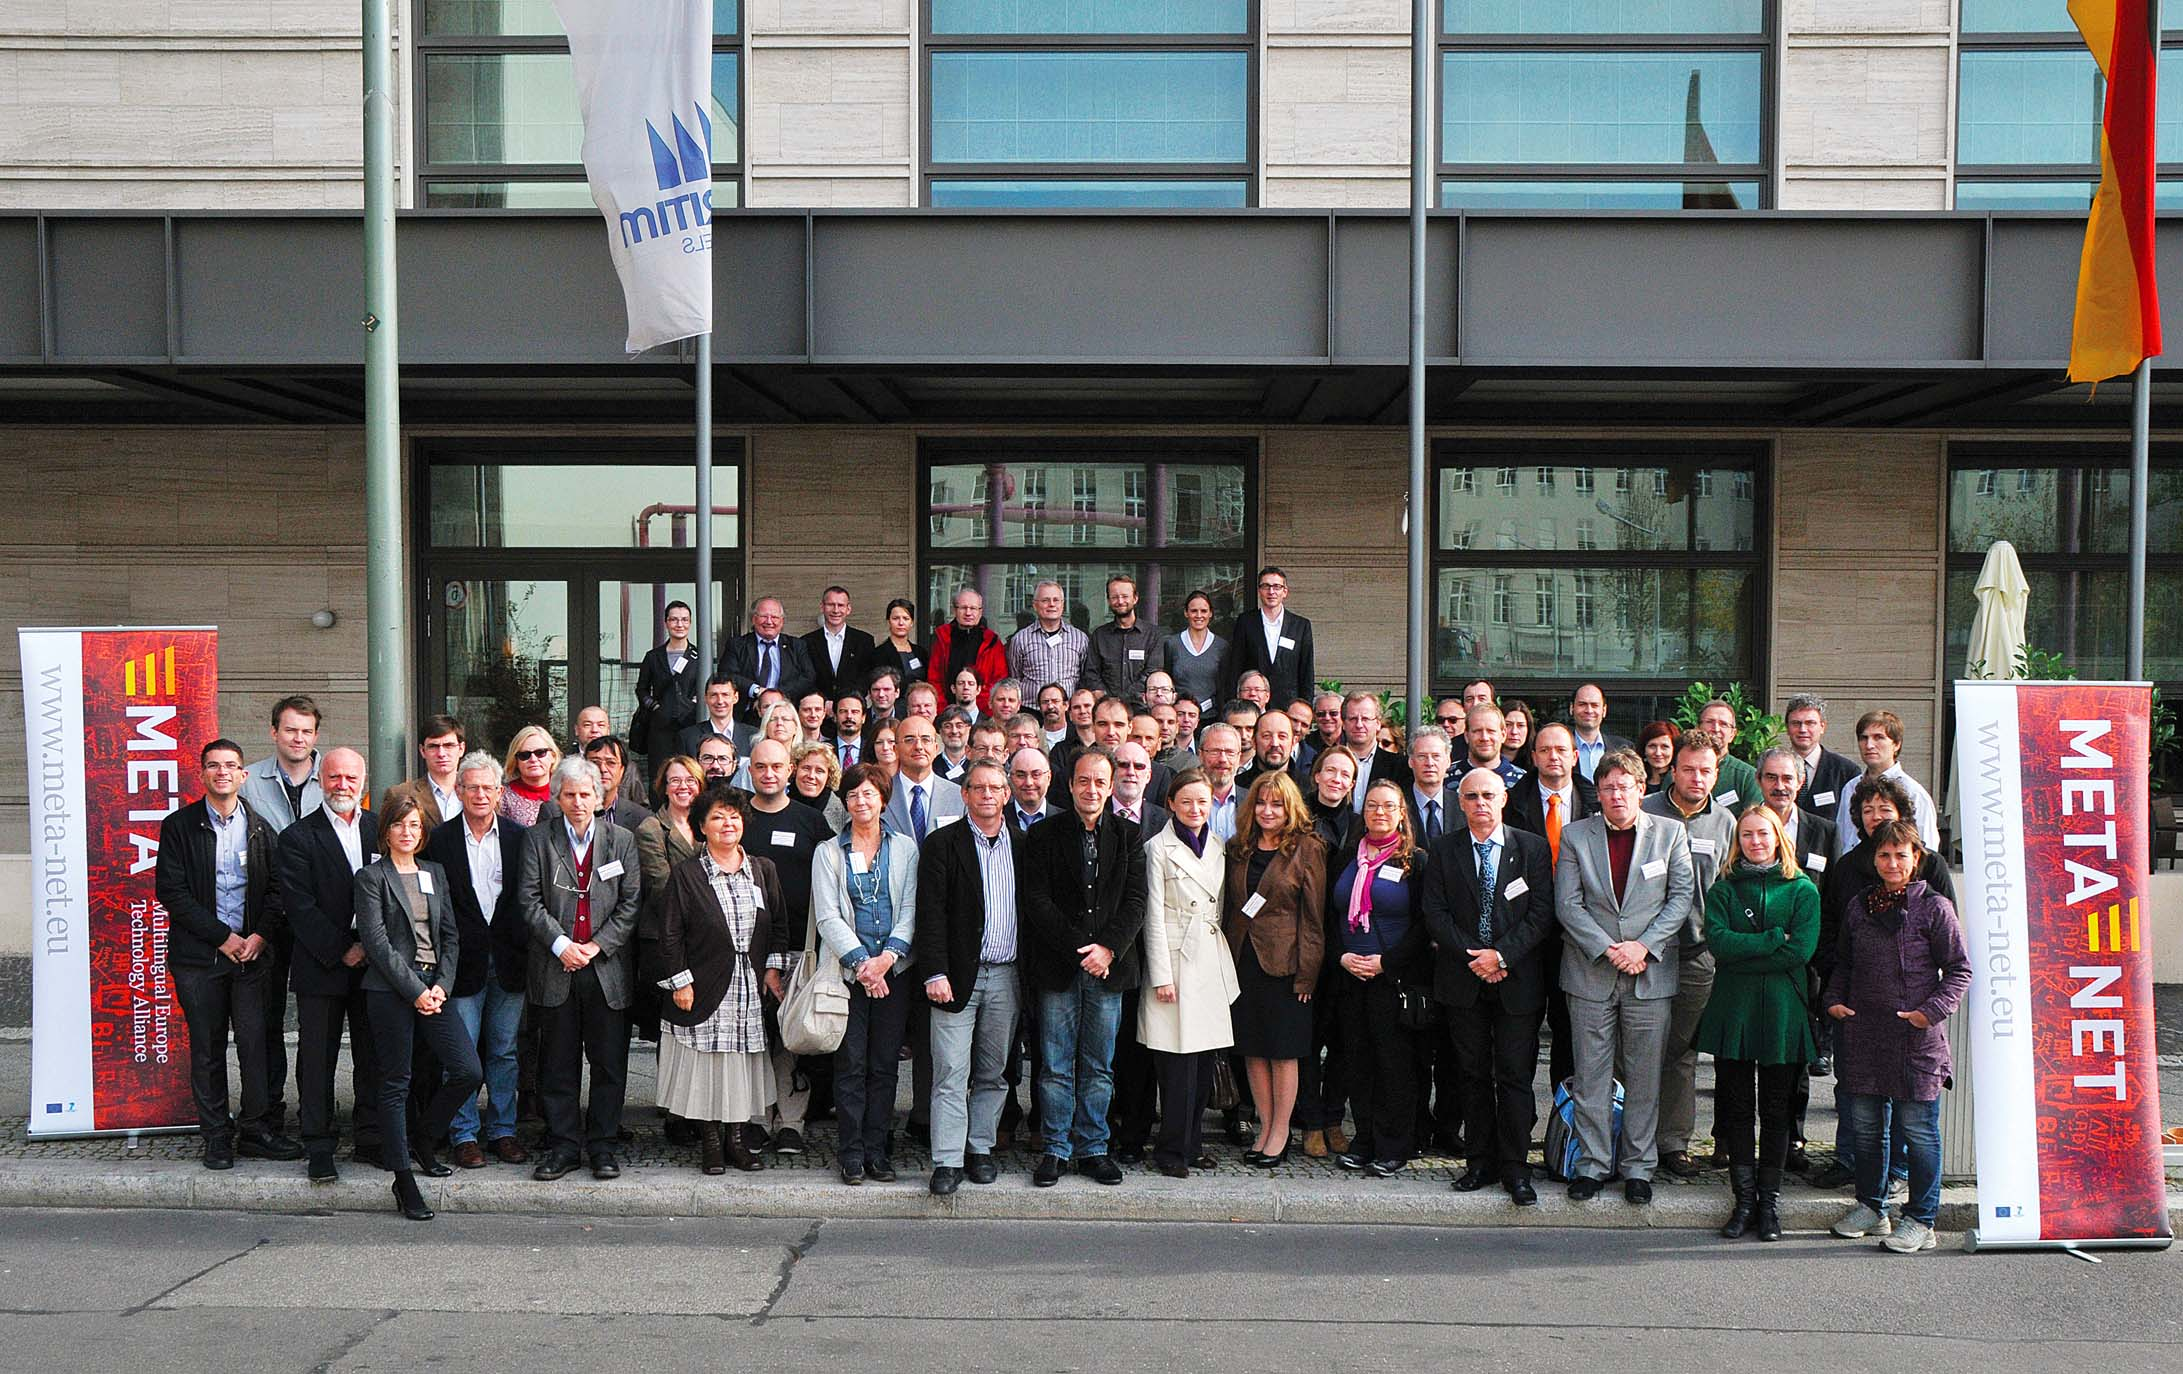
\includegraphics[width=\textwidth]{../_media/meta-net_team_ebook.jpg}
  }{%
    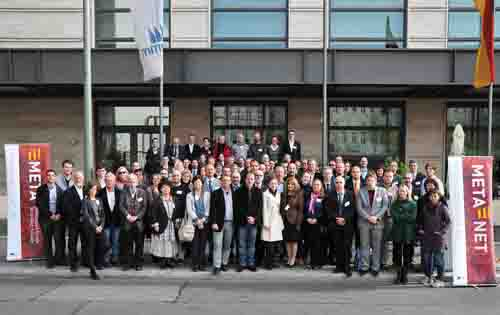
\includegraphics[width=\textwidth]{../_media/meta-net_team.jpg}
  }
  \caption{Omtrent 100 ekspertar innan språkteknologi --
    representantar for landa og språka i META-NET -- sluttførte
    diskusjonen om nøkkelresultata og -konklusjonane i kvitbokserien
    på eit META-NET-møte i Berlin, Tyskland, 21--22 oktober 2011. ---
    \textcolor{grey1}{About 100 language technology experts --
      representatives of the countries and languages represented in
      META-NET -- discussed and finalised the key results and messages
      of the White Paper Series at a META-NET meeting in Berlin,
      Germany, on October 21--22, 2011.}}
  \colorrule{grey3}{\textwidth}{1.5pt}
\end{figure*}

\cleardoublepage

\phantomsection\bsection[META-NET kvitbokserien --- The META-NET White Paper Series]{META-NET kvitbokserien --- The META-NET\ \ \ \ \ \ White Paper Series}
\label{whitepaperseries}

\vspace*{-5mm}
\centering
  \setlength{\tabcolsep}{2.6em}
  \begin{tabularx}{\textwidth}{lllll} \toprule\addlinespace
  %\begin{tabulary}{170mm}{LLL} \toprule
  &baskisk & Basque & euskara& \\
  &bokmål & Norwegian Bokmål & bokmål& \\
  &bulgarsk & Bulgarian & български& \\
  &dansk & Danish & dansk& \\
  &engelsk & English & English& \\
  &estisk & Estonian & eesti& \\
  &finsk & Finnish & suomi& \\
  &fransk & French & français& \\
  &galisisk & Galician & galego& \\
  &gresk & Greek & ελληνικά& \\
  &irsk & Irish & Gaeilge& \\
  &islandsk & Icelandic & íslenska& \\
  &italiensk & Italian & italiano& \\
  &katalansk & Catalan & català& \\
  &kroatisk & Croatian & hrvatski& \\
  &latvisk & Latvian & latviešu valoda& \\
  &litausk & Lithuanian & lietuvių kalba& \\
  &maltesisk & Maltese & Malti& \\
  &nederlandsk & Dutch & Nederlands& \\
  &nynorsk & Norwegian Nynorsk & nynorsk& \\
  &polsk & Polish & polski& \\
  &portugisisk & Portuguese & português& \\
  &rumensk & Romanian & română& \\
  &serbisk & Serbian & српски& \\
  &slovakisk & Slovak & slovenčina& \\
  &slovensk & Slovene & slovenščina& \\
  &spansk & Spanish & español& \\
  &svensk & Swedish & svenska& \\
  &tsjekkisk & Czech & čeština& \\
  &tysk & German & Deutsch& \\
  &ungarsk & Hungarian & magyar& \\ \addlinespace \bottomrule
\end{tabularx}
